\documentclass{article}
\usepackage{nth}
\usepackage{fancyhdr}
\usepackage{titlesec}
\usepackage{amsmath}
\usepackage{amssymb}
\usepackage{graphicx}
\usepackage{multirow}
\usepackage[table,xcdraw]{xcolor}
\usepackage{colortbl}
\usepackage{hyperref}
\usepackage{afterpage}
\usepackage{listings}
\usepackage{subfig}
\usepackage{enumitem}
\usepackage{tcolorbox}
\pagestyle{fancy}


\fancyhead[L]{Metodi Avanzati di Programmazione}
\fancyhead[R]{Marco Ferrara}

\setlength{\headheight}{15pt}

\title{MAP - Metodi Avanzati di Programmazione}
\author{Marco Ferrara}
\date{Marzo 2024}

\begin{document}
	\maketitle
	
	\tableofcontents
	\newpage
	
	\section{Astrazione nella progettazione}
	Il termine \textbf{astrazione} deriva dal latino \textit{asbstrahere} che vuol dire "\textit{trascinare via}", dal verbo \textit{trahere} che significa \textit{trascinare}. Intendiamo trascinare un concetto, un'idea o un principio da una realtà concreta. \\
	In ambito scientifico, astrarre significa cambiare la rappresentazione di un problema.\\
	\textit{Qual è l'obiettivo?}\\
	L'obiettivo del cambio di rappresentazione è quello di concentrarsi su \textbf{aspetti rilevanti}, tralasciando gli elementi \textit{incidentali}.
	\vspace{\baselineskip} \\
	L'astrazione si focalizza sulle caratteristiche essenziali di un oggetto, rispetto alla \textit{prospettiva} di colui che osserva.
	\vspace{\baselineskip} \\
	Il termine astrazione sottointende:
	\begin{itemize}
		\item \textbf{un processo:} l'astrazione delle informazioni essenziali e rilevanti per un particolare scopo, ignorando il resto dell'informazione.
		\item \textbf{una entità:} una descrizione semplificata di un sistema che mette in risalto alcuni dei dettagli o proprietà, trascurando il resto.
	\end{itemize}
	\textbf{Nota:} entrambi le viste sono valide.
	
	\subsection{Astrazione e software}
	Nella \textbf{programmazione} il termine astrazione fa riferimento alla distinzione tra:
	\begin{itemize}
		\item \textbf{cosa:} \textit{what} $\rightarrow$ cioè cosa fa un pezzo di codice.
		\item \textbf{come:} \textit{how} $\rightarrow$ cioè come esso è implementato. 
	\end{itemize}	
	Per l'utente del codice l'essenziale è cosa fa il codice, non è interessato ai dettagli dell'implementazione.
	\vspace{\baselineskip}\\
	Poichè i sistemi software diventano sempre più complessi, per padroneggiare la \textbf{complessità}, è neccessario che ci si concentri soltanto su pochi aspetti che interessano maggiormente il contesto.\\
	L'astrazione permette ai progettisti di sistemi software di risolvere \textit{problemi complessi} in maniera organizzata e facilmente gestibile.
	
	\subsection{Astrazione funzionale}
	L'astrazione funzionale si riferisce alla \textbf{progettazione del software}, in particolar modo alla possibilità di specificare un modulo software che vada a trasformare dei dati in input in dati di output, nascondendo quelli che sono i dettagli algoritmici della progettazione.
	\vspace{\baselineskip}\\
	Sintetizzando:
	\begin{itemize}
		\item il modulo software deve trasformare un input in un output, cioè deve calcolare una funzione;
		\item i dettagli della trasformazione (cioè del calcolo) non sono visibili al consumatore (finale) del modulo;
		\item il consumatore conosce solo le convenzioni corrette di chiamate (chiamate \textbf{specifica sintattica}) e cosa fa il modulo (chiamata \textbf{specifica semantica});
		\item il consumatore deve fidarsi del risultato.
	\end{itemize}
	\textbf{Esempio:} modulo che realizza un operatore per il calcolo del fattoriale.\\
	La \textit{specifica sintattica} indica il nome del modulo (es. fatt), il tipo di dato passato in input e il tipo di risultato che si ottiene, cosi da permettere la chiamata corretta della funzione.\\ 
	
	Ad esempio: fatt(intero) $\rightarrow$ intero 
	\vspace{\baselineskip}\\
	La \textit{specifica semantica} indica, invece, la trasformazione operata, cioè proprio la funzione calcolata: 
		\[
		fatt(n) = 
		\begin{cases}
			n \cdot (n-1) \cdot \ldots \cdot 2 \cdot 1 & \text{se n $>$= 1} \\
			1 & \text{se n = 0}
		\end{cases}
		\]
	\\ \textbf{Come specificare la semantica del modulo?}\\
	Un modo è quello di esprimere, attraverso due \textit{predicati}, la relazione che lega i dati di ingresso ai dati di uscita: se il primo predicato (detto \textbf{precondizione}) è vero sui dati in ingresso e se il programma termina su quei dati, allora il secondo predicato (detto \textbf{postcondizione}) è vero sui dati in uscita.\\Queste specifiche semnatiche sono chiamate \textbf{assiomatiche}.
	\vspace{\baselineskip}\\
	Ritornando all'esempio del fattoriale:\\
	Precondizione: $n \in \mathbb{N}$\\
	Postcondizione: 
	\[
	fatt(n) = 
	\begin{cases}
		n \cdot (n-1) \cdot \ldots \cdot 2 \cdot 1 & \text{se n $>$= 1} \\
		1 & \text{se n = 0}
	\end{cases}
	\]
	\\
	\textbf{Esercizio:} Un modulo ha in input un intero x e un vettore A di n interi. Restituisce un intero p e un vettore di B interi. \\
	Siano date le seguenti condizioni:
	\begin{itemize}
		\item Precondizione:  $ n>0  \land \forall i \in[1,n]  A[i] \in Z  $ 
		\item Postcondizione: $ \forall i \in [1,n] \exists j \in [1,n]  B[i]=A[i] \land \forall i \in[1,p-1] B[i] <= x $ 
			\newline 
			$\land \forall i \in[p+1,n] B[i]>x  $
	\end{itemize}
	Qual è la funzione in questo modulo? \\
	Continua.. \\
	
	\subsection{Limiti dell'astrazione funzionale}
	L'astrazione funzionale non permette di progettare (e quindi sviluppare) moduli software \textit{invarianti ai cambiamenti nei dati}, in quanto sono invarianti solo ai cambiamenti nei processi di trasformazione che operano. \\
	Tutto ciò rende difficoltosa la manutenzione delle soluzioni progettate e risulta inappropriata per lo sviluppo di soluzioni per problemi complessi.
	
	\subsection{Principio dell'astrazione dati}
	Alla base dell'astrazione dati c'è il principio che \textbf{non si può accedere direttamente alla rappresentazione di un dato} qualunque esso sia, ma si può accedere soltanto attraverso un insieme di operazioni che devono essere considerate lecite. \\
	Il vantaggio è che nel momento in cui c'è un cambiamento nella rappresentazione di un dato, questo si ripercuoterà soltanto sulle operazione lecite, le quali potrebbero subire delle modifiche; ma non porterà nessuna modifica sul codice che utilizza il dato astratto. 
	\vspace{\baselineskip} \\
	\textbf{Esempio:} Se i moduli "Rimuovi duplicati" e "Ricerca elemento" accedono all'elenco attraverso un insieme di operazioni (ad esempio 'dammi il prossimo elemento', o 'non ci sono più elementi'), il cambiamento della rappresentazione dell'elenco richiederà una riformulazione delle operazioni lecite ma non andrà ad influenzare i due moduli. 
	\begin{figure}[h] % Opzione [h] posiziona la figura "qui" nella pagina
		\centering
		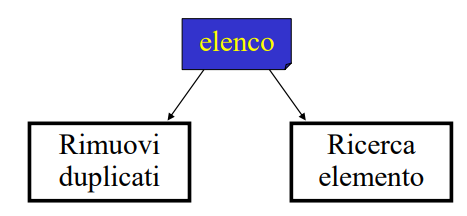
\includegraphics[width=0.5\linewidth]{assets/immagine1} 
		\caption{Esempio}
		\label{fig:etichetta}
	\end{figure}
	
	\subsection{Information Hiding}
	In generale, un principio di astrazione suggerisce di \textbf{occultare l'informazione} (\textit{information hiding}) sulla rappresentazione del dato perchè:
	\begin{itemize}
		\item non è necessaria al consumatore dell'entità astratta
		\item la sua rivelazione creerebbe delle dipendenze inutili che andrebbero a compromettere l'invarianza ai cambiamenti
	\end{itemize}
	Il principio dell'astrazione funzionale suggerisce di occultare i dettagli del processo di trasformazione, cioè come esso è operato.\\
	Il principio dell'astrazione dati identifica nella rappresentazione del dato l'informazione da nascondere. \\
	\textbf{Nota:} in entrambi i casi non si dice COME farlo.
	\begin{figure}[h] % Opzione [h] posiziona la figura "qui" nella pagina
		\centering
		
\includegraphics[width=0.2\linewidth]{assets/immagine2} 
		\caption{Information Hiding}
		\label{fig:etichetta}
	\end{figure}
	
	\subsection{Incapsulamento (encapsulation)}
	\textbf{Cos'è?} E' una tecnica di progettazione che consiste nell'\textbf{impacchettare} (o \textit{racchiudere in capsule}) una collezione di entità, andando a creare una \underline{barriera} \underline{concettuale}.
	\vspace{\baselineskip} \\
	Esso sottointende:
	\begin{itemize}
		\item \textbf{un processo:} l'impacchettamento
		\item \textbf{una entità:} il pacchetto ottenuto; ad essa corrispondono tecniche di programmazione che consentono l'incapsulamento dei dati.
	\end{itemize}
	\textbf{Esempi:}
	\begin{itemize}
		\item una procedura impachetta diversi comandi;
		\item una libreria incapsula diverse funzioni;
		\item un oggetto incapsula un dato e un insieme di operazioni sul dato.
	\end{itemize} 
	
	\noindent
	Inoltre, l'incapsulamento non dice \textit{come} devono essere le \textbf{pareti del pacchetto} o della capsula, le quali potranno essere:
	\begin{enumerate}
		\item \textbf{trasparenti:} permettono di vedere tutto quello che è stato impacchettato;
		\item \textbf{traslucide:} permettono di vedere in modo parziale il contenuto;
		\item \textbf{opache:} nascondono tutto il contenuto del pacchetto.
	\end{enumerate}
	
	\subsection{Astrazione dati AND Incapsulamento}
	Andando a combinare il principio di astrazione dati e la tecnica dell'incapsulamento, si ha che:
	\begin{itemize}
		\item la rappresentazione del dato va nascosta;
		\item L'accesso al dato deve passare solo attraverso operazioni lecite;
		\item Le operazioni lecite (che devono avere accesso all'informazione sulla rappresentazione del dato) vanno impacchettate con la rappresentazione del dato stesso.
	\end{itemize}
	\textbf{Esempio:} il dato "conto corrente" ha una sua rappresentazione interna che permette di memorizzare il \textit{saldo} (balance), il \textit{limite fido} (overcraft limit) e il \textit{numero di conto} (account number). la rappresentazione dei dati, come già detto in precedente, è nascosta e l'accesso alla rappresentazione stessa passa per quattro operazioni lecite:
	\begin{itemize}
		\item creazione conto
		\item deposito
		\item prelievo
		\item stampa saldo
	\end{itemize}
	La rappresentazione e le operazioni lecite sono impacchettate in un modulo.
	\begin{figure}[h] % Opzione [h] posiziona la figura "qui" nella pagina
		\centering
		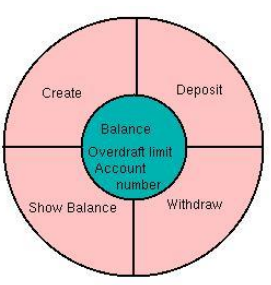
\includegraphics[width=0.3\linewidth]{assets/immagine3} 
		\caption{Esempio}
		\label{fig:etichetta}
	\end{figure}
	
	Ovviamente, l'\textit{isolamento dei moduli} \textbf{non} può essere totale. \\
	In generale, la \textbf{specifica (o contratto)} descrive come si può interagire con un dato astratto.
	
	\subsection{Astrazione dati VS Astrazione funzionale}
	L'astrazione dati ricalca ed estende quella funzionale. \\
	Attualmente la possibilità di effettuare astrazioni di dati è considerata importante almeno quanto quella di definire nuovi operatori con astrazioni funzionali. \\
	La scelta delle strutture dati è il primo passo importante per avere un buon risultato dell'attività di programmazione.
	\vspace{\baselineskip} \\
	L'\textbf{astrazione funzionale} stimola gli sforzi per evidenziare operazioni ricorrenti o comunque ben caratterizzate all'interno della soluzione del problema.
	\vspace{\baselineskip} \\
	L'\textbf{astrazione di dati} stimola, invece, in più gli sforzi per andare ad individuare le organizzazioni di dati più consone alla soluzione del problema.
	\vspace{\baselineskip} \\
	Si va quindi da una progettazione \textbf{function centered} a una \textbf{data centered}.
	
	\subsection{Punti di vista dell'astrazione}
	Solitamente, le astrazioni supportano la separazione dei diversi interessi di
	\begin{itemize}
		\item utenti: i quali sono interessati a cosa si astrae (what)
		\item implementatori: i quali sono interessati a come (how) si astrae
		\item specifica
		\item realizzazione
	\end{itemize}
	
	\subsubsection{Specifica}
	Per descrivere una specifica bisogna ricorrere a \textit{linguaggi di specifica}, i quali sono diversi dai linguaggi usati per descrivere le realizzazione delle astrazioni.
	\vspace{\baselineskip} \\
	In generale, la specifica può essere:
	\begin{itemize}
		\item \textbf{sintattica:} la quale stabilisce quali identificatori sono associati \newline all'astrazione;
		\item \textbf{semantica:} la quale definisce il risultato della computazione inclusa \newline nell'astrazione.
	\end{itemize} 
	
	\subsubsection{Parametrizzazione di un'astrazione}
	Per rendere migliore l'efficacia di un'astrazione, si possono utilizzare i \textbf{parametri} per la comunicazione con l'ambiente esterno. \\
	Quando un'astrazione viene chiamata, ogni \underline{parametro formale} viene associato al corrispondente \underline{argomento}.
	\vspace{\baselineskip} \\
	\textbf{Attenzione:} Ritornando all'astrazione dati, anche quest'ultima (come qualunque altra astrazione), è formata da una \textbf{specifica} e una \textbf{realizzazione}, dove:
	\begin{itemize}
		\item la \underline{specifica} consente di descrivere un nuovo dato e gli operatori che si possono applicare ad esso;
		\item la \underline{realizzazione} stabilisce come il nuovo dato e i nuovi operatori vengono ricondotti ai dati e agli operatori che sono già disponibili.
	\end{itemize} 
	
	\subsection{Linguaggi di specifica}
	I \textbf{linguaggi di specifica} per astrazione dati più conosciuti sono due:
	\begin{enumerate}
		\item il \textit{linguaggio logico-matematico} usato nelle asserzioni $\rightarrow$ \textbf{specifiche assiomatiche}
		\item il \textit{linguaggio dell'algebra} usato nelle equ azioni definite tra gli operatori che sono stati specificati nel dato astratto $\rightarrow$ \textbf{specifiche algebriche}
	\end{enumerate}
	
	\subsubsection{Specifiche assiomatiche}
	Parliamo di specifica assiomatica quando un linguaggio formale per la specifica di un tipo di dato astratto è formato dalla notazione logico-matematica delle \textit{asserzioni}. \\
	Una specifica assiomatica è formata da:
	\begin{enumerate}
		\item una \textit{specifica sintattica} (chiamata \underline{segnatura}), la quale fornisce 
			\begin{itemize}
				\item l'elenco dei nomi dei domini e delle operazioni specifiche del tipo
				\item i domini sia di partenza che di arrivo per ogni nome di operatore
		\end{itemize}
		\item una \textit{specifica semantica} che associa:
			\begin{itemize}
				\item un insieme ad ogni nome di tipo introdotto nella specifica sintattica
				\item una funzione ad ogni nome di operatore, esplicitando sui domini di arrivo e partenza sia la precondizione ( che definisce quando un operatore è applicabile) che la postcondizione (che stabilisce la relazione tra argomenti e risultato)
			\end{itemize}
	\end{enumerate}
	L'esempio più elementare di una specifica assiomatica è quella di un vettore.
	
	\subsubsection{Esempio: Il dato astratto Vettore}
	Definiamo la specifica sintattica e semantica.
	\begin{itemize}
		\item \textit{Specifica sintattica:} 
		\vspace{\baselineskip} \\
		Tipi: vettore, intero, tipoelem 
		\vspace{\baselineskip} \\
		Operatori:\\
		CREA VETTORE() $\rightarrow$ vettore \\
		LEGGIVETTORE(vettore, intero) $\rightarrow$ tipoelem \\
		SCRIVIVETTORE(vettore, intero, tipoelem) $\rightarrow$ vettore 
		\item \textit{Specifica semantica:} 
		\vspace{\baselineskip} \\
		Tipi: \\
		-intero: l'insieme dei numeri interi \\
		-vettore: l'insieme delle sequenze di $n$ elementi di tipo $element$ 
		\vspace{\baselineskip} \\
		Operatori: 
		\vspace{\baselineskip} \\
		CREA VETTORE = v \\
		$\rightarrow$ Pre: non ci sono precondizioni o più precisamente il predicato che definisce la precondizione di CREA VETTORE è il valore vero \\
		$\rightarrow$ Post: $\forall i \in \left\{0,1,2, \ldots, n-1\right\}$, l'$i-esimo$ elemento del vettore, $v(i)$, è uguale ad un prefissato elemento di tipo tipoelem
		\vspace{\baselineskip} \\
		LEGGIVETTORE(v,i) = e \\
		$\rightarrow$ Pre: $0 <= i <= n-1$ \\
		$\rightarrow$ Post: e=v(i)
		\vspace{\baselineskip} \\
		SCRIVIVETTORE(v,i,e) = v' \\
		$\rightarrow$ Pre: $0 <= i <= n-1$ \\
		$\rightarrow$ Post: $\forall j \in 
		\left\{0,1, \ldots, n-1\right\}, j \neq i, v'(j)=v(j), v'(i)=e$
		\item \textit{Realizzazione:} 
		\vspace{\baselineskip} \\
		In Java il vettore (chiamato \textit{array}) è un tipo di dato concreto. Vediamo la corrispondenza tra la specifica introdotta a quella del Java: \\
		
		CREA VETTORE $\leftrightarrow$ tipoelem v[n] \\
		LEGGIVETTORE(v,i) $\leftrightarrow$ v[i] \\
		SCRIVIVETTORE(v,i,e) $\leftrightarrow$ v[i]=e
	\end{itemize}
	dove $i$ può essere anche un'espressione di tipo intero.
	
	\subsubsection{Limiti delle specifiche assiomatiche}
	Notiamo che il metodo di specifiche assiomatica risulta preciso nella definizione della specifica sintattica ma risulta piuttosto informale per altri aspetti, tanto che delle volte si ricorre al linguaggio naturale per semplicità. \\
	In particolare, non consente di definire i valori che possono essere generati mediante l'applicazione di operatori e non consente di stabilire quando l'applicazione di diverse sequenze di operatori porta allo stesso valore.
	\vspace{\baselineskip} \\
	Questo problema è superato dalle \textbf{specifiche algebriche}.
	
	\subsubsection{Specifiche Algebriche}
	Le specifiche algebriche si basano sull'algebra, piuttosto che sulla logica. Essenzialmente definiscono un \textbf{dato astratto} come un'\textbf{algebra eterogenea}, ovvero come una collezione di diversi insiemi su cui sono definite diverse operazioni.
	Le algebre tradizionali sono omogenee. Un'algebra omogenea consiste in un unico insieme e diverse operazioni.
	\vspace{\baselineskip} \\
	\textbf{Esempio}: $\mathbb{Z}$  con le operazioni di addizione e moltiplicazione è un'algebra omogenea.
	\vspace{\baselineskip} \\
	\textbf{Esempio}: Dato un alfabeto $\Sigma$, indichiamo con $\Sigma^\ast $ l'insieme di tutte le stringhe, incluso quella vuota, costruite con i simboli di $\Sigma$.
	$\Sigma\ast $ con le operazioni di concatenaione e calcolo della lunghezza non sono un'algebra omogenea, visto che il codominio dell'operazione di calcolo della lunghezza è $\mathbb{N}$ e non $\Sigma^\ast$.
	Quindi quest'algebra consiste in due insiemi, stringhe e interi, su cui sono definite le operazioni di concatenamento e lunghezza delle stringhe.
	
	\paragraph{Specifica algebrica}
	Una specifica algebrica consiste in tre parti:
	\begin{enumerate}
		\item \textbf{Sintattica}: elenca i nomi del tipo, le sue operazioni e il tipo degli argomenti delle operazioni. Se un'operazione è una funzione allora è specificato il codominio (range) della funzione.
		\item \textbf{Semantica}: consiste in un insieme di equazioni algebriche che descrivono in modo indipendente dalla rappresentazione delle proprietà delle operazioni.
		\item \textbf{Di restrizione}: stabilisce varie condizioni che devono essere soddisfatte o prima che siano applicate le operazioni o dopo che esse siano state completate.
	\end{enumerate}
	Alcuni autori inglobano le specifiche di restrizione in quelle semantiche.
	\vspace{\baselineskip} \\
	Uno degli aspetti più interessanti delle specifiche algebriche è la semplicità del linguaggio di specifica rispetto ai liinguaggi di programmazione procedurale.\\
	Infatti, il linguaggio di specifica consiste in solo cinque primitive:
	\begin{enumerate}
		\item composizione funzionale:
		\item relazione di eguaglianza
		\item costante true
		\item costante false
		\item un numero illimitato di variabili libere (a differenza della specifica semantica assiomatica che definisce le variabili tramite quantificatori).
	\end{enumerate}
	La funzione matematica \textbf{\textit{if then else}}, che ha come dominio il prodotto cartesiano fra un boolean e due statement (composizioni di funzioni) e come codominio uno statement, può essere facilmente descritta dalle seguenti equazioni:
	\begin{center}
		\textit{if then else (true, q, r) = q} \\
		\textit{if then else (false, q, r) = r}
	\end{center}
	Questa funzione è così importante che si assume già data come operatore infisso:
	\begin{center}
		\textit{if p then q else r}
	\end{center}
	Inoltre si assume che sono predefiniti i valori interi e booleani.
	
	\subsection{Specifiche Algebriche}
	\subsubsection{Specifica algebrica di Pila}
	Una \textbf{pila} è una struttura dati lineare che segue il principio '\textit{LIFO}' (Last In, First Out), il che significa che l'ultimo elemento inserito è il primo ad essere rimosso. Puoi immaginare una pila come un insieme di oggetti impilati uno sopra l'altro, dove l'unico modo per accedere agli elementi è rimuovere l'elemento più recentemente inserito.
	Ogni insieme è detto \textbf{sort} (letteralmente 'tipo') dell'algebra eterogenea. I sort item e boolean sono ausiliari alla definizione di stack.
	\begin{itemize}
		\item \textbf{Specifica sintattica}:
		\begin{itemize}
			\item \textit{sorts}: stack, item, boolen
			\item \textit{operations}:
			\begin{itemize}
				\item newstack() $\rightarrow$ stack
				\item push(stack, item) $\rightarrow$ stack
				\item pop(stack) $\rightarrow$ stack
				\item top(stack) $\rightarrow$ item
				\item isnew(stack) $\rightarrow$ boolean
			\end{itemize}
		\end{itemize}
		\item \textbf{Specifica semantica}: 
		Nella specifica semantica occorre dichiarare i parametri su cui lavorano gli operatori.
		\textit{declare} \textbf{stk}: stack, \textbf{i}: item
		\begin{enumerate}
			\item pop(push(stk, i)) = stk
			\item top(push(stk,i)) = i
			\item isnew(newstack()) = true \\ newstack = newstack() in caso di assenza di parametri
			\item isnew(push(stk, i)) = false
		\end{enumerate}
		\item \textbf{Specifica di restrizione} \\ \textit{restrictions}
		\begin{itemize}
			\item pop(newstack) = error
			\item top(newstack) = error
		\end{itemize}
		dove 'error' è un elemento speciale indefinito.
	\end{itemize}
	Ovviamente avremmo potuto scrivere molte altre equazioni come:
	\begin{center}
		isnew(pop(push(newstack, i))) = true
	\end{center}
	che evidenzia come il predicato \textit{isnew} sia vero anche per quegli stack ottenuti inserendo un generico elemento \textit{i} in un \textbf{nuovo} stack e poi rimuovendolo. \\
	Tuttavia questa equazione è \textbf{ridondante}, poichè è ricavabile dalle altre scritte in precedenza. Infatti, grazie alla 1. e alla 4. equazione possiamo scrivere:
	\begin{center}
		isnew(pop(push(newstack, i))) = isnew(newstack) = true
	\end{center} 
	Nelle specifiche semantiche è importante indicare l'insieme minimale di equazioni (dette \textbf{assiomi}) a partire dalle quali possiamo derivare tutte le altre. \\
	Le specifiche si diranno:
	\begin{itemize}
		\item \textbf{incomplete} se non permetteranno di derivare tutte le equazioni desiderate dell'algebra specificate. 
		\item \textbf{inconsistenti} se permetteranno di derivare delle equazioni indesiderate. 
		\item \textbf{ridondanti} se alcune delle equazioni sono ricavabili dalle altre.
	\end{itemize}
	\paragraph*{Costruttori e Osservazioni}
	Scrivere delle specifiche semantiche complete, consistenti e non ridondanti può non essere un compito semplice. Per questo conviene introdurre una \textbf{metodologia}, che si basa sulla distinzione degli operatori di un dato astratto in:
	\begin{itemize}
		\item \textbf{Costruttori}, che creano o istanziano il dato astratto
		\item \textbf{Osservazioni}, che ritrovano informazioni sul dato astratto
	\end{itemize}
	Il comportamento di una astrazione dati può essere specificata riportando il valore di ciascuna osservazione applicata a ciascun costruttore. \\
	Questa informazione è organizzata in modo naturale nella seguente matrice:
	\begin{center}
		\begin{tabular}{|c|cc|}
		\hline
		\multirow{2}{*}{\textbf{Osservazioni}} & \multicolumn{2}{c|}{\textbf{Costruttore di stk'}} \\ \cline{2-3} 
											   & \multicolumn{1}{c|}{newstack}    & push(stk, i)   \\ \hline
		pop(stk')                              & \multicolumn{1}{c|}{error}       & stk            \\ \hline
		top(stk')                              & \multicolumn{1}{c|}{error}       & i              \\ \hline
		isnew(stk')                            & \multicolumn{1}{c|}{true}        & false          \\ \hline
		\end{tabular}
	\end{center}
	Tutte le osservazioni viste finora sono unarie, nel senso che esse osservano un singolo valore del dato astratto. Spesso è necessario disporre di osservazioni più complesse. \\
	Per confrontare due valori è necessario osservare due istanze del dato astratto. Questo complica la specifica, perchè il valore dell'osservazione dev'essere definito per tutte le \textbf{combinazioni di costruttori} possibili per i valori astratti che si devono confrontare. \\
	\vspace*{\baselineskip}	\\
	\textbf{Esempio}: predicato \textit{equal(l,m)} che è vero solo se le due pile contengono gli stessi elementi nello stesso ordine.
	Anche in questo caso possiamo organizzare il predicato in modo naturale nella seguente matrice 	che può essere vista come l'aggiunta di una terza dimensione alla tabella di base per le osservazioni unarie. \\
	Bisogna assumere and(\^): Boolean x Boolean $\rightarrow$ Boolean.
	\begin{center}			
	\begin{tabular}{|c|cc|}
	\hline
	\multirow{2}{*}{\textbf{Costruttore di m}} & \multicolumn{2}{c|}{\textbf{Costruttore di l}}                                                       \\ \cline{2-3} 
												& \multicolumn{1}{c|}{newstack} & push(stk, i)                                                         \\ \hline
	newstack                                   & \multicolumn{1}{c|}{true}     & false                                                                \\ \hline
	push(stk', i')                             & \multicolumn{1}{c|}{false}    & \begin{tabular}[c]{@{}c@{}}i=i' and \\ equal(stk, stk')\end{tabular} \\ \hline
	\end{tabular}
	\end{center}
	Questa terza dimensione può essere rimossa andando a classificare esplicitamente solo il primo argomento dell'osservazione e refereniando in modo astratto il secondo argomento mediante una variabile libera.
	\begin{center}
		\begin{tabular}{|c|cc|}
		\hline
		\multirow{2}{*}{\textbf{Osservazione}} & \multicolumn{2}{c|}{\textbf{Costruttore di stk'}}                                                                            \\ \cline{2-3} 
											   & \multicolumn{1}{c|}{newstack} & push(stk, i)                                                                                 \\ \hline
		equal(stk', m)                         & \multicolumn{1}{c|}{isnew(m)} & \begin{tabular}[c]{@{}c@{}}not isnew(m) and\\ i=top(m) and\\ equal(stk, pop(m))\end{tabular} \\ \hline
		\end{tabular}
	\end{center}

	\subsubsection{Specifica algebrica di Coda}
	Una \textbf{coda} è una struttura dati che segue il principio '\textit{FIFO}' (First In, First Out). Gli elementi vengono aggiunti alla fine della coda (operazione di "enqueue") e rimossi dall'inizio (operazione di "dequeue").
	\begin{itemize}
		\item \textbf{Specifica sintattica}:
		\begin{itemize}
			\item \textit{sorts}: queue, item, boolen
			\item \textit{operations}:
			\begin{itemize}
				\item newq() $\rightarrow$ queue
				\item addq(queue, item) $\rightarrow$ queue
				\item deleteq(queue) $\rightarrow$ queue
				\item frontq(queue) $\rightarrow$ item
				\item isnewq(queue) $\rightarrow$ boolean
			\end{itemize}
		\end{itemize}
		\begin{center}
			\begin{tabular}{|c|cc|}
			\hline
			\multirow{2}{*}{\textbf{Osservazioni}} & \multicolumn{2}{c|}{\textbf{Costruttore di q'}} \\ \cline{2-3} 
												& \multicolumn{1}{c|}{newq}    & addq(q, i)   \\ \hline
			isneq(q')                              & \multicolumn{1}{c|}{true}       & false            \\ \hline
			frontq(q')                              & \multicolumn{1}{c|}{error}       & if isnewq(q) then i else frontq(q)              \\ \hline
			delete(q')                            & \multicolumn{1}{c|}{error}        & if isnewq(q) then newq else addq(deleteq(q), i)          \\ \hline
			\end{tabular}
		\end{center}
		\item \textbf{Specifica semantica}: 
		\textit{declare} \textbf{q}: queue, \textbf{i}: item
		\begin{enumerate}
			\item isnewq(newq) = true
			\item isnewq(addq(q,i)) = false
			\item deleteq(addq(q,i)) = if isnewq(q) then newq else \\ addq(deleteq(q),i)
			\item frontq(addq(q, i)) = if isnewq(q) then i else frontq(q)
		\end{enumerate}
		\item \textbf{Specifica di restrizione} \\ \textit{restrictions}
		\begin{itemize}
			\item frontq(newq) = error
			\item deleteq(newq) = error
		\end{itemize}
	\end{itemize}
	\newpage
	\subsection{Esercizi Svolti}
	\subsubsection*{Esercizio 1: dato astratto Stringa}
	Fornire una specifica algebrica semantica completa, consistente e minimale per il dato astratto Stringa supposto che le specifiche sintattiche siano le seguenti:
	\begin{itemize}
		\item sorts: string, char, integer, boolean
		\item operations:
		\begin{itemize}
			\item new() $\rightarrow$ string //crea nuove stringhe
			\item append(string,string) $\rightarrow$ string //concatena due stringhe
			\item add(string, char) $\rightarrow$ string //aggiungere un carattere a fine stringa
			\item lenght(string) $\rightarrow$ integer //calcola la lunghezza di una stringa
			\item isEmpty(string) $\rightarrow$ boolean //predica se la stringa è vuota
			\item equal(string, string) $\rightarrow$ boolean //predica se due stringhe sono uguali
		\end{itemize}
	\end{itemize}
	Nello scegliere i costruttori adotteremo il \textbf{criterio di minimalità}, cioè l'insieme dei costruttori dev'essere il più piccolo insieme di operatori necessario a costruire tutti i possibili valori per un certo dato astratto.
	Ci poniamo 3 quesiti:
	\begin{itemize}
		\item Produce come output il sort principale?
		\item effettivamente crea un dato astratto di sort principale o lo modifica/distrugge?
		\item è atomico o è esprimibile mediante altri costruttori?
	\end{itemize}
	I candidati sono:
	\begin{itemize}
		\item new()
		\item append(string, string)
		\item add(string, char)
	\end{itemize}
	Ora, è evidente che per costruire una stringa abbiamo bisogno di:
	\begin{itemize}
		\item new() $\rightarrow$ string
		\item add(string, char) $\rightarrow$ string
	\end{itemize}
	Il terzo operatore, append(string,string) $\rightarrow$ string, non è necessario poichè semplificabile mediante add, quindi non lo scegliamo come costruttore.
	\vspace*{\baselineskip}	\\
	Per determinare il numero di espressioni che dovremo generare secondo la specifica semantica, possiamo calcolare il prodotto tra il numero di occorrenze del sort principale come parametro e il numero di costruttori del medesimo sort principale.
	In questo caso avremo 2*6 espressioni.
	\begin{itemize}
		\item Specifica Semantica
		\begin{itemize}
			\item Declare: s,s':string; c,c':char
			\begin{itemize}
				\item length(new) = 0
				\item lenght(add(s,c)) = length(s) + 1 \\
				Assumo +(Integer, Integer) $\rightarrow$ Integer
				\item isEmpty(new) = true
				\item isEmpty(add(s,c)) = false
				\item equal(new, new) = true
				\item equal(new, add(s',c')) = false
				\item equal(add(s,c), new) = false
				\item equal(add(s,c), add(s',c')) = c=c' and equal(s,s') \\
				Assumo and(Boolean, Boolean) $\rightarrow$ Booleand \\
				Assumo =(Character, Character) $\rightarrow$ Boolean
				\item append(new, new) = new
				\item append(new, add(s'.c')) = add(s',c')
				\item append(add(s,c), add(s',c')) = add(append(add(s,c), s'), c')
			\end{itemize}
		\end{itemize}
	\end{itemize}
	\newpage
	\subsubsection*{Esercizio 2: dato astratto Conto con Fido}
	Progettare il dato astratto Conto Con Fido (account with overcraft) che consente di rappresentare dei conti correnti bancari per i quali è permesso uno scoperto. Si deve poter limitare lo scoperto tramite concessione del fido. \\
	Le operazioni ammesse per questo dato astratto sono:
	\begin{itemize}
		\item conto(account): apre un nuovo conto corrente bancario definendo saldo iniziale e massimo scoperto ammesso
		\item saldo(balance): riporta il saldo del conto
		\item deposita(deposit): deposita una somma sul conto
		\item preleva(withdraw): preleva denaro dal conto
		\item concediFido(setOverdraftLimit): definisce il limite massimo dello scoperto
		\item fidoConcesso(getOverdraftLimit): restituisce il limite massimo dello scoperto
	\end{itemize}
	A partire da queste operazioni ammesse definiamo le specifiche sintattiche:
	\begin{itemize}
		\item sorts: contocorrente, saldo, denaro, scoperto
		\begin{itemize}
			\item conto(saldo,scoperto) $\rightarrow$ contocorrente
			\item saldo(contocorrente) $\rightarrow$ saldo
			\item deposita(contocorrente, denaro) $\rightarrow$ contocorrente
			\item preleva(contocorrente, denaro) $\rightarrow$ contocorrente
			\item concediFido(contocorrente, scoperto) $\rightarrow$ contocorrente
			\item fidoConcesso(contocorrente) $\rightarrow$ scoperto
		\end{itemize}
	\end{itemize}
	L'unico costruttore che definiamo è \textit{conto}. Gli altri operatori sono tutte osservazioni.
	\begin{center}
	\begin{tabular}{|c|c|}
		\hline
		\multirow{2}{*}{\textbf{Osservazioni}} & \textbf{Costruttore di c}                                                                   \\ \cline{2-2} 
											   & conto(s,l)                                                                                  \\ \hline
		saldo(c)                               & s                                                                                           \\ \hline
		deposita(c,d)                          & conto(s+d, l)                                                                               \\ \hline
		preleva(c,d)                           & \begin{tabular}[c]{@{}c@{}}if s-d\textless{}-1 then error\\ else conto(s-d, l)\end{tabular} \\ \hline
		concediFido(c,l')                      & \begin{tabular}[c]{@{}c@{}}if s\textless{}-l' then error\\ else conto(s,l')\end{tabular}     \\ \hline
		fidoConcesso(c)                        & l                                                                                           \\ \hline
		\end{tabular}
	\end{center}
	Assumo:
	\begin{itemize}
		\item declare s: Saldo;l,l':scoperto; d:denaro
		\item +(Saldo, Denaro) $\rightarrow$ Saldo
		\item -(Saldo, Denaro) $\rightarrow$ Saldo
		\item -(Scoperto) $\rightarrow$ Scoperto
		\item \textless(Saldo, Scoperto) $\rightarrow$ Boolean
	\end{itemize}
	Da qui possiamo produrre le espressioni della specifica semantica:
	\begin{itemize}
		\item declare s: Saldo;l,l':scoperto; d:denaro
		\begin{itemize}
			\item saldo(conto(s,l)) = s
			\item deposita(conto(s,l), d) = conto(s+d, l)
			\item preleva(conto(s,l), d) = if s-d\textless-l then error else conto(s-d, l)
			\item concediFido(conto(s,l), l') = if s\textless-l' then error else conto(s,l')
			\item fidoConcesso(conto(s,l)) = l 
		\end{itemize}
	\end{itemize}
	\newpage
	\subsubsection*{Esercizio 3: dato astratto Dizionario}
	Progettare il dato astratto Dizionario che consente di gestire un insieme di coppie chiave-valore.\\
	Le operazioni ammesse per questo dato astratto sono:
	\begin{itemize}
		\item creaDizionario: restituisce un dizionario vuoto
		\item aggiungiCoppia: aggiunge una coppia composta da chiave e valore al dizionario
		\item cancella: cancella tutte le occorrenze di un dato valore, restituisce errore in assenza di occorrenze da rimuovere
	\end{itemize}
	Iniziamo a definire la specifica sintattica:
	\begin{itemize}
		\item sorts: Dizionario, Chiave, Valore, Integer, Boolean
		\begin{itemize}
			\item creaDizionario() $\rightarrow$ Dizionario
			\item aggiungiCoppia(Dizionario, Chiave, Valore) $\rightarrow$ Dizionario
			\item cancella(Dizionario, Valore) $\rightarrow$ Dizionario
			\\
			\item conta(Dizionario, Valore) $\rightarrow$ Integer
		\end{itemize}
	\end{itemize}
	Come costruttore identifichiamo \textit{creaDizionario} e \textit{aggiungiCoppia}. \\
	Passiamo alla specifica semantica: \\\\
	declare d:Dizionario; k:Chiave; v,v':Valore 
	\begin{center}
		\begin{tabular}{|c|cc|}
		\hline
												& \multicolumn{2}{c|}{\textbf{Costruttore di d'}}                                                                                                                                                                     \\ \cline{2-3} 
		\multirow{-2}{*}{\textbf{Osservazioni}} & \multicolumn{1}{c|}{creaDizionario()}         & aggiungiCoppia(d,k,v)                                                                                                                                               \\ \hline
		cancella(d',v')                         & \multicolumn{1}{c|}{error}                    & \begin{tabular}[c]{@{}c@{}}if(v=v') then\\    if conta(d,v')\textgreater{}=1 then cancella(d,v')\\    else d\\ else aggiungiCoppia(cancella(d,v'),k,v)\end{tabular} \\ \hline
		{\color[HTML]{FE0000} conta(d',v')}     & \multicolumn{1}{c|}{{\color[HTML]{FE0000} 0}} & {\color[HTML]{FE0000} if(v=v') then conta(d,v')+1 else conta(d,v')}                                                                                                 \\ \hline
		\end{tabular}
	\end{center}
	Assumo +(Intero, Intero) $\rightarrow$ Intero

	\newpage

	\subsection{Esercizi}
	\subsubsection*{Esercizio 1: dato astratto Libretto}
	Fornire le specifiche algebriche del tipo astratto Libretto di cui si forniscono le specifiche sintattiche:
	\begin{itemize}
		\item sorts: Libretto, Esame, Voto, Boolean, Intero
		\item operators:
		\begin{itemize}
			\item crea() $\rightarrow$ Libretto //crea un libretto vuoto
			\item inserisci(Libretto, Esame, Voto) $\rightarrow$ Libretto //registra la coppia Esame-Voto sul libretto
			\item vuoto(Libretto) $\rightarrow$ Boolean //verifica che il libretto sia vuoto
			\item contieneEsame(Libretto, Esame) $\rightarrow$ Boolean //verifica se Esame è registato nel libretto
			\item leggiVoto(Libretto, Esame) $\rightarrow$ Voto //restituisce il voto di Esame presente in Libretto
			\item contaEsami(Libretto) $\rightarrow$ Intero //restituisce il numero di esami presenti nel libretto
			\item mediaVoti(Libretto) $\rightarrow$ Voto //restituisce la media dei voti
			\item contaVoti(Libretto, Voto) $\rightarrow$ Intero //conta il numero di esami registrati nel libretto con voto uguale a Voto
			\item stessoVoto(Libretto, Libretto, Esame) $\rightarrow$ Boolean //verifica se nei due libretti è registrato lo stesso esame con lo stesso voto
		\end{itemize}
	\end{itemize}
	Stabiliamo come costruttori \text{crea} e \text{inserisci}. \\
	Procediamo con la specifica semantica:
	\begin{itemize}
		\item declare: l,l':Libretto; e,e',e'':Esame; v,v':Voto 
		\item assumo +(Intero, Intero) $\rightarrow$ Intero
		\item assumo +(Voto, Voto) $\rightarrow$ Voto
		\item assumo /(Voto, Intero) $\rightarrow$ Voto
		\begin{itemize}
			\item vuoto(crea) = true
			\item vuoto(inserisci(l,e,v)) = false
			\item contieneEsame(crea,e) = false
			\item contieneEsame(inserisci(l,e,v),e') = if e'=e then true else contieneEsame(l,e')
			\item leggiVoto(crea,e) = error
			\item leggiVoto(inserisci(l,e,v), e') = if e=e' then v else leggiVoto(l, e') \\
			\item contaEsami(crea) = 0
			\item contaEsami(inserisci(l,e,v)) = contaEsami(l)+1
			\item mediaVoti(crea) = error
		\end{itemize}
		Inserisco nella specifica sintattica: sommaVoti(Libretto) $\rightarrow$ Voto
		\begin{itemize}
			\item sommaVoti(crea) = error
			\item sommaVoti(inserisci(l,e,v)) = if vuoto(l) then v else sommaVoti(l)+v
			\item mediaVoti(inserisci(l,e,v)) = sommaVoti(inserisci(l,e,v))/contaEsami(inserisci(l,e,v))
			\item contaVoti(crea, v) = 0
			\item contaVoti(inserisci(l,e,v),v') = if v=v' then contaVoti(l,v')+1 else contaVoti(l,v')
			\item stessoVoto(crea, crea, e) = error
			\item stessoVoto(crea, inserisci(l,e,v),e') = error
			\item stessoVoto(inserisci(l,e,v), crea, e') = error
			\item stessoVoto(inserisci(l,e,v), inserisci(l',e',v'), e'') = 
			\begin{verbatim}
				leggiVoto(inserisci(l,e,v),e'') = leggiVoto(inserisci(l',e'v'),e'')
			\end{verbatim}
		\end{itemize}
	\end{itemize}
	\newpage
	\subsubsection*{Esercizio 2: dato astratto SocialBook}
	Fornire le specifiche algebriche del tipo astratto SocialBook di cui si forniscono le specifiche sintattiche:
	\begin{itemize}
		\item sorts: SocialBook, Contatto, Intero, Boolean
		\item operators:
		\begin{itemize}
			\item crea() $\rightarrow$ SocialBook //crea un SocialBook vuoto
			\item aggiungiContatto(SocialBook,Contatto) $\rightarrow$ SocialBook //aggiunge il Contatto al SocialBook
			\item aggiungiLegame(SocialBook,Contatto,Contatto) $\rightarrow$ SocialBook //crea un legame tra i due Contatti nel SocialBook
			\item vuoto(SocialBook) $\rightarrow$ Boolean //verifica che il SocialBook sia vuoto ossia privo di contatti
			\item contieneContatto(SocialBook,Contatto) $\rightarrow$ Boolean //verifica che il Contatto appartenda al SocialBook
			\item contieneLegame(SocialBook,Contatto,Contatto) $\rightarrow$ Boolean //verifical'esistenza di un legame tra i due Contatti del SocialBook
			\item contaLegami(SocialBook,Contatto) $\rightarrow$ Intero //conta i legami in cui è coinvolto Contatto nel SocialBook, se il Contattonon appartiene al SocialBook genera errore
			\item rimuoviContatto(SocialBook,Contatto) $\rightarrow$ SocialBook //rimuove il Contatto dal SocialBook (qualora vi appartenga) e i suoi legami, se non appartiene lascia il SocialBookinalterato
			\item rimuoviLegame(SocialBook,Contatto,Contatto) $\rightarrow$ SocialBook //rimuove il legame tra due Contatti nel SocialBook, se uno dei due Contatti non appartiene al SocialBook o non esiste un legame tra i due Contatti genera errore
			\item contiene(SocialBook,SocialBook) $\rightarrow$ Boolean //restituisce vero se tutti i contatti del primo SocialBook appartengono anche al secondo SocialBook
		\end{itemize}
	\end{itemize}	
	Definiamo come costruttori \textit{crea}, \textit{aggiungiContatto} e \textit{aggiungiLegame}
	Procediamo con la specifica semantica:
	\begin{itemize}
		\item declare: s,s':SocialBook; c,c',c'',c''':Contatto
		\item Assumo l'esistenza dei seguenti operatori sui sort secondari:
		\begin{itemize}
			\item and(Boolean,Boolean) $\rightarrow$ Boolean
			\item or(Boolean,Boolean) $\rightarrow$ Boolean
			\item +(Intero,Intero) $\rightarrow$ Intero
		\end{itemize}
		\item vuoto(crea) = true
		\item vuoto(aggiungiContatto(s,c)) = false
		\item vuoto(aggiungiLegame(s,c,c')) = false
		\item contieneContatto(crea,c) = false
		\item contieneContatto(aggiungiContatto(s,c),c') = if c=c' then true else contieneContatto(s,c')
		\item contieneContatto(aggiungiLegame(s,c,c'),c'') = contieneContatto(s,c'')  //perchè aggiungiLegame non va a variare i contatti presenti
		\item contieneLegame(crea,c,c') = false
		\item contieneLegame(aggiungiContatto(s,c),c',c'') = contieneLegame(s,c',c'') //perchè c appena aggiunto non può avere legami
		\item contieneLegame(aggiungiLegame(s,c,c'), c'',c''') = 
		\begin{verbatim}
			if((c=c'' and c'=c''')or(c=c''' and c'=c'')) 
			then true
			else contieneLegame(s,c'',c''')
		\end{verbatim}
		\item rimuoviContatto(crea,c) = crea
		\item rimuoviContatto(aggiungiContatto(s,c), c') = 
		\begin{verbatim}
			if c=c' then s 
			else aggiungiContatto(rimuoviContatto(s,c'),c)
		\end{verbatim}
		\item rimuoviContatto(aggiungiLegame(s,c,c'),c'') =
		\begin{verbatim}
			if(c=c'' or c'=c'') then rimuoviContatto(s,c'')
			else aggiungiLegame(rimuoviContatto(s,c''),c,c')
		\end{verbatim}
		\item contaLegami(crea, c)= error
		\item contaLegami(aggiungiContatto(s,c),c') = if c=c' then 0 else contaLegami(s,c')
		\item contaLegami(aggiungiLegame(s,c,c'),c'') = 
		\begin{verbatim}
			if(c=c'' or c'=c'') 
			then contaLegami(s,c'')+1
			else contaLegami(s,c'')
		\end{verbatim}
		\item rimuoviLegame(crea,c,c') = error
		\item rimuoviLegame(aggiungiContatto(s,c),c',c'') = 
		\begin{verbatim}
			if(c=c' or c=c'')
			then error
			else aggiungiContatto(rimuoviLegame(s,c',c''),c)
		\end{verbatim}
		oppure
		\begin{verbatim}
			aggiungiContatto(rimuoviLegame(s,c',c''),c)
		\end{verbatim}
		\item rimuoviLegame(aggiungiLegame(s,c,c'),c'',c''') =
		\begin{verbatim}
			if((c=c'' and c'=c''')or(c=''' and c'=c''))
			then s
			else aggiungiLegame(rimuoviLegame(s,c'',c'''),c,c')
		\end{verbatim}
		\item contiene(crea,crea) = true
		\item contiene(crea,aggiungiContatto(s,c)) = true
		\item contiene(crea,aggiungiLegame(s,c,c')) = true
		\item contiene(aggiungiContatto(s,c),crea) = false
		\item contiene(aggiungiContatto(s,c), aggiungiContatto(s',c')) = 
		\begin{verbatim}
			contieneContatto(aggiungiContatto(s',c'),c) and contiene(s,aggiungiContatto(s',c'))
		\end{verbatim}
		\item contiene(aggiungiContatto(s,c), aggiungiLegame(s',c',c'')) = contiene(aggiungiContatto(s,c),s')
		\item contiene(aggiungiLegame(s,c,c'),crea) = false
		\item contiene(aggiungiLegame(s,c,c'),aggiungiContatto(s',c'')) = contiene(s,aggiungiContatto(s',c''))
		\item contiene(aggiungiLegame(s,c,c'),aggiungiLegame(s',c'',c''')) = contiene(s,s')
	\end{itemize}
	\newpage
	\subsubsection*{Esercizio 3: dato astratto Albero}
	Fornire le specifiche algebriche del tipo astratto SocialBook di cui si forniscono le specifiche sintattiche:
	\begin{itemize}
		\item sorts: Albero, Nodo, Intero, Boolean
		\item operators:
		\item +(Intero,Intero) $\rightarrow$ Intero
		\item and(Boolean,Boolean) $\rightarrow$ Boolean
		\begin{itemize}
			\item crea() $\rightarrow$ Albero //crea un albero binario vuoto
			\item aggiungiR(Albero, Nodo) $\rightarrow$ Albero // aggiunge la radice all'albero
			\item aggiungiS(Albero, Nodo, Nodo)$\rightarrow$ Albero // aggiunge il secondo nodo come figlio sinistro del primo nodo nell'albero
			\item aggiungiD(Albero, Nodo, Nodo)$\rightarrow$ Albero // aggiunge il secondo nodo come figlio destro del primo nodo nell'albero
			\item conta(Albero) $\rightarrow$ Intero // conta il numero di nodi nell'albero
			\item max(Albero) $\rightarrow$  Intero // restituisce  la profondità massima dell'albero
			\item pota(Albero, Nodo) $\rightarrow$  Albero // cancella il sottoalbero radicato nel nodo trasformandolo in foglia; solleva errore se il nodo è assente
			\item equal(Albero, Albero) $\rightarrow$  Boolean // restituisce  vero se i due alberi hanno uguale profondità massima, falso altrimenti
			
		\end{itemize}
	\end{itemize}
	Definiamo come costruttori \textit{crea}, \textit{aggiungiR}, \textit{aggiungiS} e \textit{aggiungiD}
	Procediamo con la specifica semantica:
	\begin{itemize}
		\item declare: a,a':Albero; n,n',n'',n''':Nodo
		\item Assumo l'esistenza dei seguenti operatori sui sort secondari:
		\begin{itemize}
			\item +(Intero,Intero) $\rightarrow$ Intero
			\item and(Boolean,Boolean) $\rightarrow$ Boolean
		\end{itemize}
		\item conta(crea) = 0
		\item conta(aggiungiR(a,n)) = 1
		\item conta(aggiungiS(a,n,n')) = conta(a)+1
		\item conta(aggiungiD(a,n,n')) = conta(a)+1
		\item max(crea)=0
		\item max(aggiungiR(a,n)) = 1
	\end{itemize}
	Aggiungiamo nella specifica sintattica: profondita(Albero,Nodo) $\rightarrow$ Intero
	\begin{itemize}
		\item profondita(crea,n) = 0
		\item profondita(aggiungiR(a,n), n') = if n=n' then 1 else 0
		\item profondita(aggiungiS(a,n,n'), n'') = 
		\begin{verbatim}
			if n'=n''
			then 1+profondita(a,n)
			else profondita(a,n'')
		\end{verbatim}
		\item profondita(aggiungiD(a,n,n'), n'') = 
		\begin{verbatim}
			if n'=n''
			then 1+profondita(a,n)
			else profondita(a,n'')
		\end{verbatim}
		\item max(aggiungiS(a,n,n')) = 
		\begin{verbatim}
			if(max(a)=profondita(a,n))
			then max(a)+1
			else max(a)
		\end{verbatim}
		\item max(aggiungiD(a,n,n')) = 
		\begin{verbatim}
			if(max(a)=profondita(a,n))
			then max(a)+1
			else max(a)
		\end{verbatim}
		\item pota(crea,n) = error
		\item pota(aggiungiR(a,n),n') = if n=n' then aggiungiR(a,n) else error
		\item pota(aggiungiS(a,n,n'),n'') = 
		\begin{verbatim}
			if n'=n'' 
			then aggiungiS(a,n,n') 
			else 
				if n=n''
				then pota(a,n'')
				else 
					if antenato(a,n'',n)
					then pota(a,n'')
					else aggiungiS(pota(a,n''),n,n')
		\end{verbatim}
		\item pota(aggiungiD(a,n,n'),n'') = 
		\begin{verbatim}
			if n'=n'' 
			then aggiungiD(a,n,n') 
			else 
				if n=n''
				then pota(a,n'')
				else 
					if antenato(a,n'',n)
					then pota(a,n'')
					else aggiungiD(pota(a,n''),n,n')
		\end{verbatim}
	\end{itemize}
	Aggiungiamo nella specifica sintattica: antenato(Albero,Nodo,Nodo) $\rightarrow$ Boolean
	\begin{itemize}
		\item antenato(crea,n,n') = error
		\item antenato(aggiungiR(a,n),n',n'') = error
		\item antenato(aggiungiS(a,n,n'),n'',n''') = 
		\begin{verbatim}
			if n=n'' and n'=n'''
			then true 
			else 
				if(appartiene(a,n'') and appartiene(a,n''')) 
				then antenatoBis(a,n'', padre(a,n'''))
				else error
			
		\end{verbatim}
		\item antenato(aggiungiD(a,n,n'),n'',n''') = 
		\begin{verbatim}
			if n=n'' and n'=n'''
			then true 
			else 
				if(appartiene(a,n'') and appartiene(a,n''')) 
				then antenatoBis(a,n'', padre(a,n'''))
				else error
		\end{verbatim}
	\end{itemize}
	Aggiungiamo nella specifica sintattica: appartiene(Albero,Nodo) $\rightarrow$ Boolean
	\begin{itemize}
		\item appartiene(crea(), n) = false
		\item appartiene(aggiungiR(a,n),n')= n=n'
		\item appartine(aggiungiS(a,n,n'),n'')=if n'=n'' then true else appartiene(a,n'')
		\item appartine(aggiungiD(a,n,n'),n'')=if n'=n'' then true else appartiene(a,n'')	
	\end{itemize}
	Aggiungiamo nella specifica sintattica: antenatoBis(Albero,Nodo,Nodo) $\rightarrow$ Boolean
	\begin{itemize}
		\item antenatoBis(crea(),n,n') = false
		\item antenatoBis(aggiungiR(a,n),n',n'') = false
		\item antenatoBis(aggiungiS(a,n,n'),n'',n''') =
		\begin{verbatim}
			if n=n'' and n'=n'''
			then true 
			else antenatoBis(a,n'', padre(a,n'''))
		\end{verbatim}
		\item antenatoBis(aggiungiD(a,n,n'),n'',n''') =	
		\begin{verbatim}
			if n=n'' and n'=n'''
			then true 
			else antenatoBis(a,n'', padre(a,n'''))
		\end{verbatim}
	\end{itemize}
	Aggiungiamo nella specifica sintattica: padre(Albero,Nodo) $\rightarrow$ Boolean
	\begin{itemize}
		\item padre(crea,n,n') = error
		\item padre(aggiungiR(a, n), n', n'') = error
		\item padre(aggiungiS(a, n, n'), n'', n''') = 
		\begin{verbatim}
			if(n=n'' and n'=n''') 
			then true 
			else padre(a, n'', n''')
		\end{verbatim}
		\item padre(aggiungiD(a, n, n'), n'', n''') =
		\begin{verbatim}
			if(n=n'' and n'=n''') 
			then true 
			else padre(a, n'', n''')
		\end{verbatim}
		\item equal(crea,a)= (max(a)=0)
		\item equal(aggiungiR(a,n),a') = (max(a')=1)
		\item equal(aggiungiS(a,n,n'),a') = (max(aggiungiS(a,n,n')) = max(a'))
		\item equal(aggiungiD(a,n,n'),a') = (max(aggiungiD(a,n,n')) = max(a'))
	\end{itemize}
	\newpage
	\subsubsection*{Esercizio 4: dato astratto Matrice}
	Fornire le specifiche algebriche del tipo astratto Matrice di cui si forniscono le specifiche sintattiche:
	\begin{itemize}
		\item sorts: Matrice, Intero, Boolean, Reale
		\item operators:
		\begin{itemize}
			\item creaMatrice(Intero) $\rightarrow$ Matrice // crea una matrice quadrata di reali (inizialmente pari a zero), la dimensione della matrice è specificata come parametro
			\item assegna(Matrice, Intero, Intero, Reale) $\rightarrow$ Matrice // assegna in valore specificato (quarto parametro) alla posizione della matrice (primo parametro) con indice di riga e colonna specificati come secondo e terzo parametro, rispettivamente
			\item leggi(Matrice, Intero, Intero) $\rightarrow$ Reale // legge il valore nella posizione della matrice con indice di riga e colonna specificati come secondo e terzo parametro, rispettivamente
			\item max(Matrice) $\rightarrow$ Reale  // restituisce il valore massimo attualmente memorizzato nella matrice
			\item somma(Matrice, Matrice) $\rightarrow$ Matrice // restituisce la matrice computata tramite somma, solleva errore se le due matrici non hanno uguale dimensione
			\item uguale(Matrice, Matrice) $\rightarrow$ Booleano // vero se le due matrici contengono uguali valori nelle medesimi posizioni, falso altrimenti (solleva errore se le due matrici non hanno uguale dimensione)
		\end{itemize}
	\end{itemize}
	Definiamo come costruttori gli operatori \textit{creaMatrice} e \textit{assegna}. \\
	Passiamo alla specifica semantica:
	\begin{itemize}
		\item declare: m,m':Matrice; r,r',c,c',d,d':Intero; v,v':Reale
		\item Assumo che siano definite le seguenti operazioni:
		\begin{itemize}
			\item $\leq$(Intero,Intero) $\rightarrow$ Boolean
			\item $<$(Intero,Intero) $\rightarrow$ Boolean
			\item and(Boolean,Boolean) $\rightarrow$ Boolean
			\item $>$(Reale,Reale) $\rightarrow$ Boolean
			\item $+$(Reale,Reale) $\rightarrow$ Reale
		\end{itemize}
		\item leggi(creaMatrice(d),r,c) = 
		\begin{verbatim}
			if r<=d and c<=d and r>0 and c>0 
			then 0 
			else error
		\end{verbatim}
		\item leggi(assegna(m,r,c,v),r',c') =
		\begin{verbatim}
			if r=r' and c=c'
			then v
			else leggi(m,r',c')
		\end{verbatim}
		\item max(creaMatrice(d)) = 0.0
		\item max(assegna(m,r,c,v)) = if max(m) $>$ v then max(m) else v
		\item somma(creaMatrice(d), creaMatrice(d')) = 
		\begin{verbatim}
			if d = d' 
			then creaMatrice(d) 
			else error
		\end{verbatim}
		\item somma(creaMatrice(d), assegna(m,r,c,v)) = 
		\begin{verbatim}
			if d = dimensione(m) 
			then assegna(m,r,c,v)
			else error
		\end{verbatim}
		\item somma(assegna(m,r,c,v), creaMatrice(d)) =
		\begin{verbatim}
			if d = dimensione(m) 
			then assegna(m,r,c,v)
			else error
		\end{verbatim}		
		\item somma(assegna(m,r,c,v), assegna(m',r',c',v')) = 
		\begin{verbatim}
			if dimensione(m) =dimensione(m') 
			then if (r=r' and c=c') 
				 then assegna(somma(m,m'),r,c,v+v')
				 else modifica(somma(assegna(m,r,c,v),m'),r',c',v'+leggi(m,r,c))
			else error
		\end{verbatim}
	\end{itemize}
	Aggiungiamo nella specifica sintattica: dimensione(Matrice) $\rightarrow$ Intero
	\begin{itemize}
		\item dimensione(creaMatrice(d)) = d
		\item dimensione(assegna(m,r,c,v)) = dimensione(m)
	\end{itemize}
	Aggiungiamo nella specifica sintattica: modifica(Matrice,Intero,Intero,Reale) $\rightarrow$ Matrice
	\begin{itemize}
		\item modifica(creaMatrice(d),r,c,v) =
		\begin{verbatim}
			if r<=d and c<=d and r>0 and c>0 
			then assegna(creaMatrice(d),r,c,v)
			else error
		\end{verbatim} 
        \item modifica(assegna(m,r,c,v),r',c',v') = 
		\begin{verbatim}	
			if r=r' and c=c'
			then assegna(m,r,c,v')
			else assegna(modifica(m,r',c',v'),r,c,v)
		\end{verbatim}
		\item uguale(creaMatrice(d), creaMatrice(d')) = if d = d' then true else error
		\item uguale(creaMatrice(d), assegna(m,r,c,v)) = 
		\begin{verbatim}
			if d = dimensione(m) 
			then else (m'=crea(d) and v=0) 
			else error
		\end{verbatim}
		\item uguale(assegna(m,r,c,v), creaMatrice(d')) = 
		\begin{verbatim}
			if d' = dimensione(m) 
			then (m=crea(d') and v=0)
			else error 
		\end{verbatim}
		\item uguale(assegna(m,r,c,v), assegna(m',r',c',v')) = 
		\begin{verbatim}
			if (dimensione(m) != dimensione(m')) 
			then error 
			else 
				if (r=r' and c=c') then 
					if (v=v') 
					then uguale(m,m') 
					else false
				else 
					if(leggi(m,r',c')=v' and leggi(m',r,c)=v) 
					then uguale(modifica(m,r',c',0),modifica(m',r,c,0))
					else false
		\end{verbatim}
	\end{itemize}

	\newpage
	\section{Astrazione nella programmazione}
	\subsection{Introduzione}
	Negli anni '50 e '60 si verificarono importanti sviluppi nei linguaggi di programmazione che introdussero diverse forme di astrazione. Queste astrazioni comprendevano la creazione di strutture di controllo, operatori e dati, che consentivano ai programmatori di gestire in modo più efficiente e chiaro la complessità dei loro programmi.
	In questo contesto, si consolidò la convinzione che fosse possibile costruire astrazioni su una vasta gamma di costrutti sintattici, a condizione che questi costrutti specificassero un qualche tipo di computazione.
	\\
	Nel corso di questo capitolo, esamineremo l'applicazione di questo principio di astrazione a sei classi sintattiche fondamentali:
	\begin{itemize}
		\item \textbf{Espressione} $\rightarrow$ Astrazione di funzione: Un'espressione rappresenta un calcolo che restituisce un valore. L'astrazione di funzione consiste nell'organizzare e incapsulare un insieme di operazioni in una singola entità, la funzione, che può essere chiamata con uno o più argomenti per ottenere un risultato specifico.
		\item \textbf{Comando} $\rightarrow$ Astrazione di procedura: Un comando rappresenta un'azione che deve essere eseguita. L'astrazione di procedura consiste nell'incapsulare una sequenza di comandi in una procedura, che può essere chiamata per eseguire l'insieme di operazioni definite.
		\item \textbf{Controllo di sequenza} $\rightarrow$ Astrazione di controllo: Il controllo di sequenza determina l'ordine in cui vengono eseguite le istruzioni. L'astrazione di controllo coinvolge la creazione di strutture di controllo più complesse, come cicli e condizioni, che consentono di gestire il flusso di esecuzione del programma in modo più flessibile e dinamico.
		\item \textbf{Accesso a un'area di memoria} $\rightarrow$ Astrazione di selettore: L'accesso a un'area di memoria implica l'individuazione e la manipolazione di dati memorizzati in variabili o strutture dati. L'astrazione di selettore coinvolge la creazione di meccanismi per accedere e manipolare queste aree di memoria in modo strutturato e controllato.
		\item \textbf{Definizione di un dato} $\rightarrow$ Astrazione di tipo: La definizione di un dato specifica la struttura e il comportamento di un tipo di dato. L'astrazione di tipo coinvolge la definizione di nuovi tipi di dato e le operazioni associate a essi, consentendo di organizzare e manipolare i dati in modi significativi e consistenti.
		\item \textbf{Dichiarazione} $\rightarrow$ Astrazione generica: Una dichiarazione introduce un'entità nel contesto del programma, come una variabile, una costante o una funzione. L'astrazione generica coinvolge la creazione di meccanismi per associare un nome a un'entità e specificarne le proprietà e il comportamento, contribuendo così alla gestione e all'organizzazione del codice.
	\end{itemize}
	È importante notare che tutte queste classi sintattiche sottintendono una forma di computazione, in quanto ogni astrazione implica l'esecuzione di operazioni o l'elaborazione di dati per ottenere un risultato. Tuttavia, esiste un controesempio: la classe sintattica "letterale", che non può essere astratta poiché rappresenta semplicemente un valore senza specificare alcuna operazione o computazione associata.

	\subsection{Astrazione di funzione}
	Un'\textbf{astrazione di funzione} rappresenta un concetto fondamentale nella programmazione, permettendo di organizzare e riutilizzare logiche di calcolo complesse in maniera efficiente e chiara. Questa astrazione è formalizzata attraverso la definizione di una funzione, che specifica come una determinata espressione deve essere valutata in base a un insieme di parametri forniti.
	\\
	La definizione di una funzione segue uno schema ben definito, del tipo:
	\[
	\text{{function }} I(FP1, ..., FPn) \text{{ is }} E
	\]
	dove:
	\begin{itemize}
		\item $I$ è l'identificatore della funzione;
		\item $FP1, ..., FPn$ sono i parametri formali della funzione, ossia i valori che devono essere forniti quando la funzione viene chiamata;
		\item $E$ è l'espressione da valutare, che rappresenta l'algoritmo o la logica di calcolo che la funzione deve eseguire.
	\end{itemize}
	In questo modo, si crea un legame tra l'identificatore della funzione e un'entità astratta che, una volta chiamata con i parametri appropriati, restituisce un valore come risultato.
	\\
	Una chiamata di funzione, del tipo $I(AP1, ..., APn)$, in cui $AP1, ..., APn$ sono i parametri effettivi che determinano gli argomenti, può essere considerata da due punti di vista:
	\begin{itemize}
		\item Dal punto di vista dell'utente, la chiamata di una funzione trasforma gli argomenti forniti in un risultato utile per il contesto del programma.
		\item Dal punto di vista dell'implementatore, la chiamata valuta l'espressione $E$, avendo precedentemente associato i parametri formali agli argomenti forniti.
	\end{itemize}
	L'algoritmo codificato nell'espressione $E$ è di particolare interesse per l'implementatore, poiché rappresenta la logica di calcolo specifica che viene eseguita quando la funzione viene chiamata. Questo algoritmo può essere complesso o semplice a seconda delle necessità, ma il suo corretto funzionamento è fondamentale per garantire il comportamento desiderato della funzione nel contesto del programma.
	\vspace{\baselineskip} \\
	Le funzioni, come astrazioni di espressioni, possono comparire ovunque si richieda un'espressione. Pertanto, possono essere utilizzate alla destra di operazioni di assegnazione, ma anche come parametri effettivi nelle chiamate di altre funzioni o procedure, dove un valore può essere calcolato mediante un'espressione. Ad esempio:
	\[
	y := f(y, \text{{power}}(x,2))
	\]
	Qui, la funzione \( f \) ha due parametri passati per valore.
	\vspace{\baselineskip} \\
	In molti linguaggi di programmazione è possibile definire dei parametri formali che sono un riferimento a una funzione. Ad esempio, in Pascal:
	\begin{verbatim}
	function Sommatoria(F:function(R:real,M:integer):real;X:real;N:integer):real;
	var
		I: integer;
		Sum: real;
	begin
		Sum := 0;
		for I := 1 to N do
			Sum := Sum + F(X, I);
		Sommatoria := Sum;
	end;
	\end{verbatim}
	Qui, la funzione \texttt{Sommatoria} prende come primo parametro una funzione \( F \), e la utilizza per calcolare una sommatoria.
	\vspace{\baselineskip} \\
	In alcuni linguaggi di programmazione, il concetto di astrazione di funzione è separato dal concetto di binding a un identificatore. Ciò permette di passare come parametri delle funzioni anonime, prive di identificatore.
	\vspace{\baselineskip} \\
	Infine, le funzioni possono essere il risultato di valutazioni di espressioni o possono essere assegnate a variabili. Ad esempio, in ML:
	\[
	\text{{val cube = fn}} (x: \text{{real}}) \rightarrow x \times x \times x
	\]
	Qui, è definita una funzione anonima, \texttt{cube}, che calcola il cubo di un numero.
	\vspace{\baselineskip} \\
	\subsubsection{Anomalie di progetto dei linguaggi}
	Se un'astrazione di funzione include un'espressione $E$ da valutare, ci si aspetterebbe naturalmente che il corpo della funzione non contenga comandi che modificano lo stato di un sistema, come assegnazioni, istruzioni di salto o iterazioni, poiché il ruolo principale di una funzione è quello di produrre valori.\\
	Tuttavia, non sempre ciò avviene, come evidenziato in questo esempio di funzione scritta in Pascal:
	\begin{verbatim}
	function power(x: real; n: integer): real
	begin
		if n = 1 then
			power := x
		else
			power := x * power(x, n - 1)
	end
	\end{verbatim}
	Nel corpo della funzione Pascal compaiono comandi di assegnazione. Questo avviene perché in Pascal, per restituire un valore, è necessario assegnare quel valore a una pseudo-variabile con lo stesso nome della funzione.
	In questo esempio, l'identificatore della funzione, \texttt{power}, funge sia da espressione da valutare che da pseudo-variabile dove verrà depositato il risultato.
	Anche se il corpo della funzione è sintatticamente un comando, semanticamente è considerato un'espressione, poiché la funzione può essere invocata solo alla destra di operazioni di assegnazione.
	\vspace{\baselineskip} \\
	È possibile evitare comandi nel corpo delle funzioni. Ad esempio, nel linguaggio funzionale ML:
	\begin{verbatim}
	function power(x: real; n: int) is
		if n = 1 then x
		else x * power(x, n - 1)
	\end{verbatim}
	Nel corpo della funzione definita in ML compare una semplice espressione condizionale, la cui valutazione non modifica lo stato del sistema.\\
	Tuttavia, linguaggi come Pascal, Ada e altri permettono comandi nel corpo delle funzioni per sfruttare la potenza espressiva dell'assegnazione e dell'iterazione nella computazione dei risultati. Altrimenti, saremmo costretti a esprimere le espressioni da valutare in modo ricorsivo, il che può essere inefficiente nell'uso delle risorse di calcolo.
    \vspace{\baselineskip} \\
	In conclusione, molti linguaggi consentono comandi nel corpo delle funzioni per motivi di efficienza, ma è compito del programmatore utilizzarli correttamente per evitare effetti collaterali oltre a quelli previsti per il calcolo del valore.

	\subsubsection{Riepilogo}
	In alcuni linguaggi di programmazione, come Fortran e Ada-83, le funzioni sono considerate di terza classe, il che significa che possono essere solo chiamate e non possono essere utilizzate in altri contesti.
	\vspace{\baselineskip} \\
	In altri linguaggi, come Pascal, le funzioni sono considerate di seconda classe, il che significa che possono essere passate come argomenti a altre funzioni o procedure, ma non possono essere restituite come risultato di una chiamata di funzione o assegnate come valore a una variabile.
	\vspace{\baselineskip} \\
	Tuttavia, in alcuni linguaggi di programmazione avanzati, come Lisp, ML e alcuni linguaggi di scripting come Perl, le funzioni sono considerate di prima classe. Questo significa che possono essere trattate allo stesso modo delle altre entità del linguaggio, come numeri o stringhe. Possono essere restituite come risultato di una chiamata di funzione, assegnate come valore a una variabile, e persino generate al runtime, permettendo un'elevata flessibilità e capacità di astrazione nel codice.
	\vspace{\baselineskip} \\
	La differenza tra i diversi livelli di "classe" delle funzioni nei linguaggi di programmazione riflette le diverse filosofie di design e le esigenze dei programmatori in termini di espressività e flessibilità nel linguaggio.

	\subsection{Cittadini di prima classe}
	In programmazione, un'entità è considerata cittadino di prima classe quando gode di piena libertà nel suo utilizzo, senza essere soggetta a restrizioni particolari. Ciò significa che l'entità può essere trattata allo stesso modo di altre entità del linguaggio, come numeri o stringhe, e può essere manipolata in modo flessibile e dinamico all'interno del programma. Questa libertà di utilizzo fornisce ai programmatori una maggiore espressività e capacità di astrazione nel codice, consentendo di scrivere software più conciso, modulare ed efficiente.
	\vspace{\baselineskip} \\
	A tal proposito, i valori possono essere classificati in base a diverse proprietà:
	\begin{itemize}
		\item \textbf{Denotabili}: I valori sono denotabili se possono essere associati ad un nome, consentendo ai programmatori di fare riferimento a essi all'interno del codice.
		\item \textbf{Esprimibili}: I valori sono esprimibili se possono essere il risultato di un'espressione complessa, diversa da un semplice nome. Questo significa che possono essere calcolati o generati mediante operazioni o combinazioni di altri valori.
		\item \textbf{Memorizzabili}: I valori sono memorizzabili se possono essere assegnati e conservati in una variabile, consentendo ai programmatori di accedervi e modificarli durante l'esecuzione del programma.
	\end{itemize}
	Ad esempio, nei linguaggi imperativi, i valori di tipo intero sono generalmente denotabili, esprimibili e memorizzabili. \\
	Al contrario, i valori del tipo delle funzioni da Integer a Integer sono denotabili in quasi tutti i linguaggi, perché possiamo dare loro un nome con una dichiarazione:
	\begin{center}
		int succ(int x) { return x+1 }
	\end{center}
	ma non sono esprimibili o memorizzabili nei linguaggi imperativi, poiché non possono essere restituiti come risultato di un'espressione complessa o assegnati a una variabile.
	\vspace{\baselineskip} \\
	La situazione è diversa nei linguaggi funzionali, come Scheme, ML e Haskell, dove i valori funzionali sono denotabili, esprimibili e, in certi linguaggi, memorizzabili. Stessa cosa dicasi per gli oggetti ai quali si accennerà in seguito. Nei linguaggi imperativi essi sono denotabili ma non esprimibili e memorizzabili. In altri termini, gli oggetti non sono cittadini di prima classe. Al contrario, nei linguaggi orientati agli oggetti, gli oggetti sono denotabili, esprimibili e memorizzabili, cioè sono cittadini di prima classe.

	\subsection{Astrazione di procedura}
	Un'astrazione di procedura include un comando da eseguire e, quando chiamata, aggiorna le variabili che rappresentano lo stato del sistema. È specificata mediante una definizione di procedura, del tipo:
	\[
		\text{{procedure }} I(FP_1; \ldots; FP_n) \text{{ is }} C
	\]
	dove:
	\begin{itemize}
		\item \(I\) è l'identificatore della procedura;
		\item \(FP_1; \ldots; FP_n\) sono i parametri formali della procedura, ossia i valori che devono essere forniti quando la procedura viene chiamata;
		\item \(C\) è il blocco di comandi da eseguire, che rappresenta l'algoritmo o la logica di calcolo che la procedura deve eseguire.
	\end{itemize}
	In questo modo, si lega \(I\) all'astrazione di procedura, che cambia lo stato del sistema quando chiamata con argomenti appropriati.
	\vspace{\baselineskip} \\
	Data una chiamata di procedura \(I(AP_1; \ldots; AP_n)\) dove \(AP_1; \ldots; AP_n\) sono i parametri effettivi, il punto di vista dell'utente è che la chiamata aggiorni lo stato del sistema in modo dipendente dai parametri, mentre il punto di vista dell'implementatore è che la chiamata consenta l'esecuzione del corpo di procedura \(C\), avendo precedentemente vincolato i parametri formali agli argomenti corrispondenti. L'algoritmo codificato in \(C\) è di interesse solo per l'implementatore.\\
	In linguaggi come Pascal e C, le procedure sono considerate cittadini di seconda classe.

	\subsubsection*{Esempio di puntatori a funzione in C}
	La funzione \texttt{bubble} ordina un array di interi sulla base di una funzione di ordinamento. L'argomento con puntatore a funzione:
	\begin{center}
		\texttt{void bubble(int a[], int n, int (*compare)(int, int, int *))}
	\end{center}
	indica a \texttt{bubble} di aspettarsi un puntatore a una funzione, identificata da \texttt{compare}, che accetti tre argomenti in ingresso e restituisca un tipo \texttt{void}.
	\vspace{\baselineskip} \\
	\textbf{Nota}: Se avessimo rimosso le parentesi:
	\[
	\texttt{void *compare(int, int, int *)}
	\]
	avremmo dichiarato semplicemente una funzione che accetta tre interi in input e restituisce un puntatore a \texttt{void}. Invece, con le parentesi, stiamo dichiarando un puntatore a funzione.

	\lstinputlisting[language=C]{assets/bubble.c}

	\subsection{Astrazione Funzionale}
	L'astrazione di funzione o di procedura sono due tecniche di programmazione di supporto all'astrazione funzionale, intesa come tecnica di progettazione del software secondo la quale occorre distinguere la specifica di un operatore (come esso è visto e manipolato dall'utente) dalla sua realizzazione.
	\vspace{\baselineskip} \\
	La scelta della tecnica di programmazione più opportuna da adottare dipende da diversi fattori:
	\begin{itemize}
		\item Il tipo di operatore progettato:
		\begin{itemize}
			\item Se l'operatore ha effetti collaterali, come modificare lo stato del sistema, è più opportuno utilizzare l'astrazione di procedura.
			\item Se l'operatore non ha effetti collaterali e restituisce un risultato senza modificare lo stato del sistema, è preferibile utilizzare l'astrazione di funzione.
		\end{itemize}
		\item I limiti imposti dal linguaggio di programmazione:
		\begin{itemize}
			\item Ad esempio, se l'operatore bubblesort non modifica l'array passato in ingresso ma ne restituisce uno ordinato, sarebbe più opportuno implementarlo ricorrendo a un'astrazione di funzione, poiché restituisce un nuovo valore che è un intero array ordinato.
			\item Tuttavia, non tutti i linguaggi di programmazione permettono di definire funzioni che restituiscono dati complessi. In alcuni linguaggi, come Pascal, gli array sono cittadini di seconda classe e in tal caso, l'operatore bubblesort dovrà essere necessariamente realizzato mediante astrazione di procedura.
		\end{itemize}
	\end{itemize}

	\subsection{Astrazione di controllo}
	L'astrazione di controllo si applica alla classe sintattica delle strutture di controllo. Queste definiscono l'ordine in cui le singole istruzioni o gruppi di istruzioni (unità di programma) devono essere eseguiti.
	\vspace{\baselineskip} \\
	Nei linguaggi di basso livello, come i linguaggi assemblativi, le istruzioni sono eseguite in sequenza e i salti sono implementati tramite istruzioni di salto, ad esempio 
	\begin{center}jump to $<$indirizzo simbolico o label$>$\end{center}
	Tuttavia, l'indirizzo simbolico è di scarsa importanza per il programmatore; ciò che conta è poter indicare le prossime istruzioni da eseguire.
	\vspace{\baselineskip} \\
	Per questa ragione i linguaggi di alto livello hanno introdotto strutture di controllo astratte per semplificare la programmazione.\\\\
	Ad esempio, l'istruzione
	\begin{center}if cond then S1 else S2\end{center}
	rappresenta una selezione astratta, mentre l'istruzione
	\begin{center}jump on $<$cond$>$ to A; S2; jump to B; A: S1; B: ...\end{center}
	rappresenta un salto astratto.
	\vspace{\baselineskip} \\
	Similmente, sono state introdotte diverse strutture di controllo astratte per l'iterazione. Inoltre, l'utilizzo dello stack per conservare gli indirizzi di ritorno dalle chiamate di funzione/procedura ha reso possibili le chiamate ricorsive.
	\vspace{\baselineskip} \\
	Di particolare interesse è l'attuale tendenza a offrire strutture di controllo iterative per collezioni omogenee di valori, come insiemi, multiinsiemi, liste e array. Ad esempio, in Java è disponibile l'astrazione di controllo "for-each", che permette di iterare su una collezione.
	\begin{center}
		\begin{verbatim}
			LinkedList<Integer> list = new LinkedList<Integer>();
			... /* si inseriscono degli elementi
			for (Integer n : list) {
				System.out.println(n);
			}
		\end{verbatim}
	\end{center}
	L'operazione messa a disposizione di LinkedList per l'astrazione di controllo for-each è iterator().
	\vspace{\baselineskip} \\
	Se consideriamo le strutture di controllo come espressioni che definiscono l'ordine di esecuzione dei comandi, possiamo specificare un'astrazione di controllo come segue:
	\[
	\text{{control }} I(FP_1; \ldots; FP_n) \text{{ is }} S
	\]
	dove:
	\begin{itemize}
		\item \(I\) è l'identificatore di una nuova struttura di controllo;
		\item \(FP_1; \ldots; FP_n\) sono i parametri formali;
		\item \(S\) è un'espressione di controllo che definisce l'ordine di esecuzione.
	\end{itemize} 
	\paragraph*{Esempio: (in un ipotetico linguaggio di programmazione)}
	\begin{verbatim}
	control swap(boolean:cond, statement:S1,S2) is 
	//argomento di tipo espressione, statement
		if cond then
			begin S1;S2 end
		else
			S2;S1
		endif
	\end{verbatim}
	La chiamata swap(i<j, {i:=j}, {j:=i}) porta i al valore di j se i è minore di j, altrimenti porta j al valore di i.

	\paragraph*{Esempio: (in un ipotetico linguaggio di programmazione)}
	\begin{verbatim}
	control alt_execution(statement: S1,S2,S3) is
	\\argomento di tipo statement
		if abnormal (S1) then
			S2
		else
			S3
		endif
	\end{verbatim}
	abnormal è un predicato che ha in input un comando S1 e restituisce true se l'esecuzione di S1 è terminata in modo anomalo (è stata sollevata un'eccezione), false altrimenti.
	\vspace{\baselineskip} \\
	I linguaggi di programmazione moderni sono dotati di meccanismi sofisticati per gestire situazioni eccezionali, tra cui errori aritmetici, errori di I/O, fallimento di precondizioni e condizioni imprevedibili. Quando si verifica un'eccezione, è necessario catturarla e gestirla in modo appropriato.
	\vspace{\baselineskip} \\
	I metodi per individuare il gestore dell'eccezione possono includere la ricerca nel blocco corrente di codice, l'uscita dall'unità corrente o la navigazione verso l'alto nella gerarchia delle unità chiamanti. Una volta individuato il gestore e gestita l'eccezione, è possibile scegliere di ripartire dall'unità contenente il gestore (nel modello di terminazione, come in Ada) o di tornare all'esecuzione del comando che ha generato l'eccezione (nel modello di ripresa).
	\vspace{\baselineskip} \\
	Nei linguaggi di programmazione sequenziale, la sequenza, la selezione e la ripetizione stabiliscono un ordinamento totale sulla sequenza di esecuzione dei comandi. Nei linguaggi paralleli, vengono impiegati ulteriori costrutti di controllo del flusso, come fork, cobegin e cicli for paralleli, per introdurre un ordinamento parziale sulla sequenza di esecuzione dei comandi. Dato che il parallelismo costituisce una forma di controllo della sequenza di esecuzione, l'astrazione di controllo assume una particolare importanza nella programmazione parallela.

	\subsection{Astrazione di selettore}
	Un linguaggio di programmazione dispone di costrutti per poter accedere in memoria ad una variabile (strutturata e non).\\
	Il selettore variabile può essere utilizzato sia in espressioni che in comandi. Per esempio, in un assegnamento, quando è a sinistra è veramente un selettore perchè deve accedere ad un'area di memoria per scrivere il dato preso. Quando è a destra è un selettore perchè deve accedere ad un'area di memoria per leggere il dato.
	Lo stesso identificatore può essere usato sia come nome di un valore (legame dinamico fra identificatore e valore) e sia come un indirizzo (legame statico fra identificatore e locazione di memoria). 
	\vspace{\baselineskip} \\
	Ad esempio in Pascal abbiamo:
	\begin{figure}[h]
		\centering
		\subfloat[]{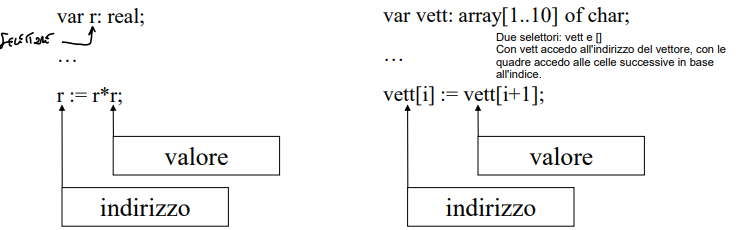
\includegraphics[width=1\textwidth]{assets/selettore1}} \hfill
		\subfloat[]{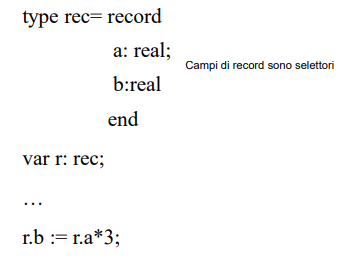
\includegraphics[width=0.5\textwidth]{assets/selettore2}}
		\caption{Due immagini affiancate.}
		\label{fig:subfig}
	\end{figure}
	\vspace{\baselineskip} \\
	Nel caso dell'array dell'immagine a abbiamo due selettori: la variabile vett che è un selettore classico che mi permette di accedere in memoria alla posizione dell'array; le parentesi quadre che mi permettono di accedere in memoria al valore dell'array in una determinata cella dipesa dall'indice di posizione. \\
	Nel caso del record dell'immagine b abbiamo i campi dei record che sono selettori e che costituiscono un riferimento ad una variabile.
	\vspace{\baselineskip} \\
	Tuttavia, se osserviamo il seguente codice Pascal:
	\begin{verbatim}
	type queue = ...;
	
	var Aq: queue;
	
	function first(q: queue): integer
		...(* Restituisce il primo intero della coda *)
	
	i := first(Aq);
	\end{verbatim}
	Ci accorgiamo che la chiamata a \texttt{first(Aq)} può comparire solo alla destra di un'assegnazione, perché le funzioni restituiscono valori, mentre a sinistra:
	\begin{verbatim}
	first(Aq) := 0;
	\end{verbatim}
	dovrebbe restituire riferimenti ad aree di memoria.
	\vspace{\baselineskip} \\
	In Pascal, abbiamo dei selettori predefiniti dal progettista del linguaggio:
	\begin{itemize}
		\item \texttt{F\^}: riferimento a un puntatore \texttt{F}
		\item \texttt{V[E]}: riferimento a un elemento di un array \texttt{V}
		\item \texttt{R.A}: riferimento a un elemento di un record
	\end{itemize}
	Tuttavia, il programmatore non ha modo di definire un nuovo selettore, come il riferimento a una lista di elementi indipendentemente da come la lista è realizzata. In altri termini, non c'è la possibilità di definire astrazioni di selettore che restituiscano l'accesso a un'area di memoria.
	\vspace{\baselineskip} \\
	Per poter scrivere un'assegnazione del tipo:
	\begin{verbatim}
	first(Aq) := 0;
	\end{verbatim}
	dovremmo poter definire un tipo di astrazione che, quando chiamata, restituisce il riferimento a una variabile (astrazione di selettore). Supponiamo di estendere il Pascal con le astrazioni di selettore nel seguente modo:
	\begin{verbatim}
	selector I(FP1; ...; FPn) is A
	\end{verbatim}
	dove \texttt{A} è un'espressione che restituisce un accesso a una variabile (che denoteremo con \& come in C).
	\vspace{\baselineskip} \\
	Potremmo allora definire \texttt{first} come segue:
	\begin{verbatim}
	type
		queue = record
			elementi: array[1..max] of integer;
			testa, fondo, lung: 0..max;
		end;

	selector first(q: queue) is &(q.elementi[q.testa]);
	\end{verbatim}
	Questo ci consentirebbe di scrivere espressioni come:
	\begin{verbatim}
	first(Aq) := first(Aq) + 1;
	\end{verbatim}
	dove l'invocazione di destra si riferisce alla funzione, mentre quella di sinistra si riferisce all'astrazione di selettore.

	\paragraph*{Esempio: Coda}
	\begin{verbatim}
		class Queue{
			\dots
			public:
				static int & first(Queue*);
		};
		Queue q*;
		\dots
		int i=first(q);
		first(q)*=first(q);
		first(q)++;
	\end{verbatim}
	dove \& è l'operatore di indirizzamento, obbligatorio per rendere la funzione un selettore.

	\subsection{Flessibilità dei linguaggi}
	La potenza espressiva di un linguaggio di programmazione è determinata principalmente da tre fattori fondamentali: i meccanismi di composizione, i meccanismi di controllo di sequenza e la gestione dei dati.
	\vspace{\baselineskip} \\
	I meccanismi di composizione si riferiscono alla capacità del linguaggio di definire operazioni complesse combinando quelle più semplici. Linguaggi che supportano l'astrazione funzionale offrono una grande flessibilità in questo ambito, consentendo ai programmatori di creare strutture complesse e modulari attraverso l'uso di funzioni e procedure.
	\vspace{\baselineskip} \\
	I meccanismi di controllo di sequenza riguardano la capacità di stabilire l'ordine di esecuzione delle istruzioni nel programma. Linguaggi che supportano l'astrazione di controllo forniscono agli sviluppatori una vasta gamma di costrutti per gestire il flusso del programma in modo chiaro e intuitivo.
	\vspace{\baselineskip} \\
	Infine, la gestione dei dati si riferisce alla capacità del linguaggio di rappresentare e manipolare i dati in modi diversi. Linguaggi che supportano l'astrazione dei dati consentono ai programmatori di definire nuovi tipi di dati e operazioni su di essi, offrendo così una maggiore flessibilità nell'organizzazione e nella manipolazione delle informazioni.

	\subsection{Tecniche di programmazione a supporto dell'astrazione dati}
	Le tecniche di programmazione che supportano l'astrazione dei dati nel paradigma imperativo, fondamentali per la progettazione del software, possono essere suddivise in due approcci principali:
	\begin{enumerate}
		\item \textbf{Definizione di Tipi Astratti}: Questo approccio consiste nell'astrazione della classe sintattica del tipo, cioè la creazione di tipi di dati personalizzati che nascondono la loro implementazione interna. Gli utenti possono interagire con questi tipi di dati attraverso un insieme di operazioni definite, senza avere conoscenza diretta della rappresentazione interna dei dati. Inoltre, i tipi astratti rendono visibili sia l'identificatore di tipo che gli operatori associati.
		\item \textbf{Definizione di Classi di Oggetti}: In questo approccio, l'astrazione si basa sulla creazione di moduli dotati di stato locale, noti come classi di oggetti. Le classi di oggetti consentono di definire oggetti che incapsulano sia i dati che le operazioni che possono essere eseguite su di essi. Tuttavia, a differenza dei tipi astratti, le classi di oggetti rendono visibili solo gli operatori associati, nascondendo l'identificatore di tipo agli utenti.
	\end{enumerate}
	In entrambi i casi, è fondamentale poter incapsulare la rappresentazione dei dati con le operazioni legittime, garantendo così un'interfaccia coerente e sicura per l'accesso e la manipolazione dei dati.
	
	\subsection{Tipo concreto e tipo astratto}
	Nei linguaggi di programmazione ad alto livello, viene fornito al programmatore un insieme diversificato di tipi predefiniti, noti come tipi concreti. Questi tipi possono essere suddivisi in due categorie principali: primitivi o semplici, i cui valori sono atomici e non possono essere ulteriormente scomposti, e composti o strutturati, i cui valori sono ottenuti dalla combinazione di valori più semplici.
	\vspace{\baselineskip} \\
	Tuttavia, l'espressività di un linguaggio di programmazione dipende anche dalla sua capacità di consentire al programmatore di definire i propri tipi di dati personalizzati a partire dai tipi di dato concreti disponibili. Questi tipi definiti dall'utente, noti anche come user defined types (UDT), sono considerati astratti in quanto nascondono i dettagli implementativi sottostanti e forniscono un'interfaccia chiara e coesa per l'interazione con i dati.

	\subsection{Astrazione di tipo}
	L'espressione di tipo (spesso abbreviato con tipo) è il costrutto con cui alcuni linguaggi di programmazione consentono di definire un nuovo tipo.
	\\Prendiamo ad esempio il linguaggio Pascal, dove possiamo creare un nuovo tipo chiamato "Person" attraverso la seguente dichiarazione:
	\begin{verbatim}
	type Person = record
	name: packed array[1..20] of char;
	age: integer;
	height: real
	end
	\end{verbatim}
	In questa dichiarazione, definiamo esplicitamente una rappresentazione per i valori del tipo "Person", specificando i campi "name", "age", e "height". Tuttavia, gli operatori associati a questo tipo saranno necessariamente generici, come ad esempio l'assegnazione. Non abbiamo la possibilità di definire operatori specifici per il tipo "Person".
	\vspace{\baselineskip} \\
	D'altra parte, l'astrazione di tipo, o tipo astratto di dato, ci permette di definire sia una rappresentazione per un insieme di valori, sia le operazioni applicabili a questi valori. Questo concetto può essere espresso attraverso una dichiarazione del tipo:
	\begin{center}
	type I(FP1; ...; FPn) is T
	\end{center}
	dove:
	\begin{itemize}
		\item "I" è l'identificatore del nuovo tipo;
		\item "FP1; ...; FPn" sono i parametri formali;
		\item "T" è un'espressione di tipo che specifica la rappresentazione dei dati di tipo "I" e le operazioni ad esso applicabili.
	\end{itemize}
	Consideriamo ad esempio l'astrazione di tipo definita per un tipo "complex":
	\begin{verbatim}
	type complex = record
	Re: real;
	Im: real
	end
	\end{verbatim}
	Qui stabiliamo che "complex" è un identificatore di tipo, e associamo una rappresentazione attraverso tipi concreti già disponibili nel linguaggio. Le operazioni associate al tipo "complex" sono quelle definite per il tipo "record", come l'assegnazione e la selezione di campi.
	\vspace{\baselineskip} \\
	Tuttavia, questa astrazione di tipo ha dei limiti evidenti:
	\begin{enumerate}
	    \item Il programmatore non può definire nuovi operatori specifici da associare al tipo.
	    \item Si viola il requisito di protezione, in quanto l'utilizzatore è consapevole della rappresentazione del tipo "complex" e può operare su di esso con operatori non specifici del dato.
	    \item L'astrazione di tipo non è parametrizzata, quindi la comunicazione con il contesto esterno è limitata.
	\end{enumerate}

	\subsection{Package}
	Per superare questi limiti, possiamo introdurre un costrutto di programmazione che permette di incapsulare rappresentazioni del dato e operatori leciti: il package. Un package è un gruppo di componenti dichiarate, come tipi, costanti, variabili, funzioni e persino (sotto) moduli. \\
	Introducendo un costrutto package, possiamo migliorare notevolmente questo concetto, consentendo una maggiore modularità, incapsulamento e flessibilità nel definire nuovi tipi di dati e le operazioni ad essi associate.
	\begin{figure}[h]
		\centering
		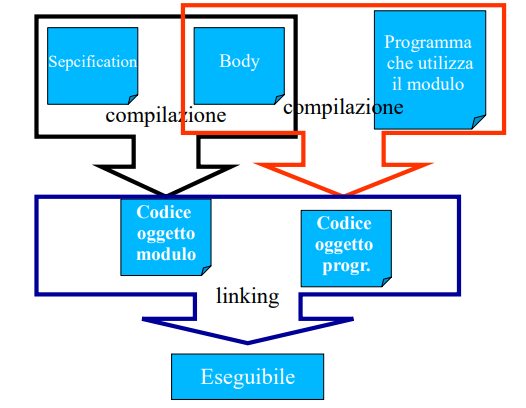
\includegraphics[width=0.5\linewidth]{assets/package} 
		\caption{}
		\label{fig:etichetta}
	\end{figure}
	\vspace{\baselineskip} \\
	In Ada, il modulo è chiamato \textit{package} e si compone di due parti:
	\begin{itemize}
		\item \textit{specification}: contiene le dichiarazioni di tipi, costanti, procedure e funzioni, e interagisce con l'ambiente esterno.
		\item \textit{body}: contiene l'implementazione di procedure e funzioni dichiarate nella \textit{specification}, ed eventualmente una routine di inizializzazione del package.
	\end{itemize}
	La \textit{specification} si articola in due sottoparti: \textit{visible} e \textit{private}.
	\begin{itemize}
	    \item Le entità dichiarate nella parte \textit{visible} possono essere rese note ad altre unità di programma mediante la clausola \texttt{use}.
	    \item Le entità dichiarate nella parte \textit{private} non possono essere né esportate né dichiarate nel corpo.
	\end{itemize}
	La parte di specifica inizia con la parola chiave package seguita dall'identificatore del package e da is; seguono poi le dichiarazioni delle entità visibili e private
	\paragraph{Esempio: Package per il tipo astratto Complex}
	\begin{verbatim}
	package Type_complex is
	    type Complex is record
	        RL, IM: Real;
	    end record;
	    I: constant Complex := (0.0, 1.0);
	    function "+"(x, y: Complex) return Complex;
	    ...
	end Type_complex;
	\end{verbatim}
	Questo è un esempio di specifica di un package che realizza il tipo astratto Complex pubblicando sia il tipo ma anche la sua implementazione poichè non c'è una parte privata nella specifica. Di conseguenza, un programma che fa uso di questo package può operare su variabili complesse mediante espressioni come la seguente:
	\begin{center}
		C.IM := C.IM + 1.0;		
	\end{center}
	invece di ricorrere alla forma più astratta:
	\begin{center}
		C:= C + I;
	\end{center}
	Per evitare il problema possiamo nascondere la struttura del tipo Complex nella parte privata.
	\paragraph{Esempio: Nascondere la Struttura di Complex nella Parte Privata}
	\begin{verbatim}
	package Type_complex is
	    type Complex is private;
	    I: constant Complex;
	    function "+"(x, y: Complex) return Complex;
	    ...
	private
	    type Complex is record
	        RL, IM: Real;
	    end record;
	    I: constant Complex := (0.0, 1.0);
	end Type_complex;
	\end{verbatim}
	Avendo dichiarato il tipo Complex nella parte privata non è	più possibile inizializzare la costante I nella parte pubblica, in quanto non è ancora nota la rappresentazione di Complex.
	\vspace{\baselineskip} \\
	Il corpo del package fornisce le implementazioni delle procedure e funzioni dichiarate nella \textit{specification}.
	\begin{verbatim}
	package body Type_complex is
	    function "+"(x, y: in Complex) return Complex is
	    begin
	        return (x.RL + y.RL, x.IM + y.IM);
	    end "+";
	    ...
	end Type_complex;
	\end{verbatim}
	Ovviamente la struttura del tipo Complex è visibile alla parte body del package, quindi si potrà accedere ai campi RL e IM dei record Complex. \\
	Il package potrà essere utilizzato come segue:
	\begin{verbatim}
	with Type_complex; use Type_complex;
	procedure main is
	    cpx1, cpx2: Complex;
	begin
	    ...
	    cpx1 := cpx2 + I;
	    ...
	end main;
	\end{verbatim}
	Si osservi che sia nella specifica e sia nel corpo di $Type\_complex$ non c'e alcuna dichiarazione di variabili esterne a procedure e funzioni. Ciò vuol dire che questo package non è dotato di uno stato locale, cioè non definisce un oggetto. Per questa ragione il corpo del package non necessita di un "main": non si deve inizializzare un oggetto. Il package puo in ogni caso avere un proprio main. Esso verra specificato dopo le varie procedure e funzioni e sara compreso fra un begin e l'end del package.
	\begin{verbatim}
	with Simple_io; use Simple_io;
	package body Type_complex is
	function "+"(x,y: in Complex) return Complex is
		begin
			return(x.RL+y.RL, x.IM+y.IM);
	end "+";
	…
	begin
	put(“Main of package Type_complex ”);
	end Type_complex;
	\end{verbatim}
	L'esecuzione del main del package avverrà al momento in cui si importa il package mediante la clausola use. Si vedrà quindi visualizzare la frase “Main of package $Type\_complex$”.

	\paragraph*{Esempio: Astrazione di Tipo per la Pila}
	\begin{verbatim}
	package Type_stack is    //il nome del package può essere casuale
	    type Stack is private; //il nome del dato astratto è da rispettare
	    procedure push(s: in out Stack; x: in Integer);
	    procedure pop(s: in out Stack);
	    procedure top(s: in Stack; x: out Integer);
	    function empty(s: in Stack) return Boolean;
	private
	    max: constant := 100;
	    type Stack is limited record
			// limited perchè mancano gli operatori uguale e assegnamento
	        st: array(1..max) of Integer;
	        top: Integer range 0..max := 0;
	    end record;
	end Type_stack;

	package body Type_stack is
	    procedure push(s: in out Stack; x: in Integer) is
	    begin
	        s.top := s.top + 1;
	        s.st(s.top) := x;
	    end push;
	    procedure pop(s: in out Stack) is
	    begin
	        s.top := s.top - 1;
	    end pop;
	    procedure top(s: in Stack; x: out Integer) is
	    begin
	        x := s.st(s.top);
	    end top;
	    function empty(s: in Stack) return Boolean is
	    begin
	        return (s.top = 0);
	    end empty;
	end Type_stack;
	\end{verbatim}
	Le specifiche del tipo astratto Pila prevedono anche un costruttore CreaPila, che non ha un corrispondente nella definizione del tipo astratto Stack perchè si utilizzano costruttori impliciti forniti da Ada, come la dichiarazione di una variabile di tipo Stack. Tuttavia se un costruttore dovesse essere parametrizzato sarà necessario prevedere un metodo. \\
	\vspace{\baselineskip} \\
	In Ada, definendo un tipo come private è possibile applicare su istanze di quel tipo tutti i metodi definiti nella parte pubblica della specifica, ma anche effettuare assegnazioni e confronti di (dis-)uguaglianza. \\
	Queste operazioni che il compilatore offre 'gratuitamente' per un tipo privato devono necessariamente essere definite in modo generale, indipendentemente da come il tipo è poi definito. Quindi saranno implementate semplicemente copiano o confrontando byte a byte le aree di memoria riservate a due dati dello stesso tipo dichiarato come privato.
	\vspace{\baselineskip} \\
	Utilizzando le operazioni predefinite potrebbero causare dei problemi:
	\begin{enumerate}
		\item l'assegnazione (:=), il confronto di eguaglianza (=) e il confronto per diseguaglianza (/=) potrebbero non far parte della specifica di un dato astratto. Quindi potrebbe non essere corrette offrirle all'utilizzatore del tipo dichiarato come privati;
		\item la semantica delle operazioni potrebbe essere diversa da quella stabilita dal compilatore
	\end{enumerate}
	Per esempio:
	\begin{verbatim}
		with Type_stack, use Type_stack;
		procedure main is
		    s1, s2: Stack;
			cmp: Boolean;
		begin
		    push(s1, 1);
		    push(s2, 1);
			push(s1, 2);
			pop(s1);
			cmp := s1 = s2;
		end main;
	\end{verbatim}
	Il valore di cmp è false. Infatti i corrispondenti campi top dei record s1 e s2 sarebbero identici, mentre non avrebbero gli stessi valori i corrispondenti campi. Eppure i due stack sarebbero identici secondo la specifica algebrica di \textit{equal(l,m)} data nel progetto.
	\vspace{\baselineskip} \\
	Per evitare tutto ciò, è sufficiente dichiarare il tipo come \textbf{limited private}, che inibisce l'uso delle operazioni di assegnazione e confronto offferte per default dal compilatore.
	\begin{verbatim}
		package Type_stack is
		    type Stack is limited private;
		    procedure push(s: in out Stack; x: in Integer);
			procedure pop(s: in out Stack);
			procedure top(s: in Stack; x: out Integer);
			function empty(s: in Stack) return Boolean;
		...		
	\end{verbatim}
	In ADA è anche possibile definire \textbf{oggetti}, cioè moduli dotati di stato locale.\\
	Per esempio, possiamo definire un oggetto di tipo Stack come segue:
	\begin{verbatim}
	package Stack is
	    procedure push(x: in Integer);
	    procedure pop;
	    procedure top(x: out Integer);
	    function empty return Boolean;
	end Stack;
	package body Stack is
		max: constant := 100;
		type Table is array(1..max) of Integer;
		st: Table;
		top: Integer range 0..max := 0;

		procedure push(x: in Integer) is
		begin
		    top := top + 1;
		    st(top) := x;
		end push;

		procedure pop is
		begin
		    top := top - 1;
		end pop;

		procedure top(x: out Integer) is
		begin
		    x := st(top);
		end top;

		function empty return Boolean is
		begin
		    return (top = 0);
		end empty;
	end Stack;
	\end{verbatim}
	Si potrà quiindi utilizzare l'oggetto Stack come segue:
	\begin{verbatim}
	with Stack; use Stack;
	procedure main is
	begin
	...
	    push(1);
	    push(2);
	    pop;
	    if empty then push(1);
	...
	end main;
	\end{verbatim}
	In generale, un oggetto è un insieme di variabili interne ad un modulo e manipolabili esternamente solo mediante gli operatori (pubblici) definiti nel modulo stesso. \\
	Per poter definire più oggetti simili o dello stesso tipo, cioè con medesima rappresentazione e stesso insieme di operatori, si è costretti a definire tanti moduli quanti sono gli oggetti che si vogliono usare nel programma. Tutti questi moduli differiranno solo per l'identificatore del modulo (\textbf{identificatore dell'oggetto}). \\
	Per evitare l'inconveniente di dover duplicare un modulo si può pensare di definire un \textbf{package generico} che identifica una \textbf{classe} di oggetti simili. I singoli oggetti sono poi ottenuti con il meccanismo della \textbf{istanziazione} della classe.
	\vspace{\baselineskip} \\
	In ADA un package che specifica e implementa un singolo oggetto può essere facilmente trasformato in un \textbf{generic package}, che definisce una classe di oggetti, premettendo la parola \textbf{generic} alla dichiarazione del modulo.
	\begin{verbatim}
		generic
		package Stack 
			procedure push(x: in Integer);
	\end{verbatim}
	In questo modo si definisce solo una matrice degli oggetti da creare. Per ottenere i singoli oggeti dobbiamo \textbf{istanziare} il generic package:
	\begin{verbatim}
		package Stack1 is new Stack
		package Stack2 is new Stack
	\end{verbatim}
	Queste due dichiarazioni sono processate in fase di precompilazione. In particolare, per ogni occorrenza di istanziazione:
	\begin{itemize}
		\item si sostituisce la stringa dell'istanziazione con il comando di importazione di un package avente come nome quello dell'istanza (with Stack1; use Stack1;)
		\item si genera un package (non generico) utilizzando il generic package come matrice. Esso si ottiene rimuovendo la parola generic e sostituendo il nome dell'istanza al posto del nome del package. Il package è poi compilato separatamente.
	\end{itemize}
	Nell'esempio specifico, la precompilazione genera due package distinti, che variano solo nel nome del package, cioè nell'\textit{identificatore dell'oggetto}.
	\vspace{\baselineskip} \\
	Possiamo, quindi, osservare che:
	\begin{itemize}
		\item il package generico non è compilabile separatamente in quanto il nome del package non identifica un oggetto
		\item la generazione di package distinti, uno per ogni istanziazione, comporta la creazione di molteplici copie dello stesso codice (inefficienza di spazio)
		\item la creazione dei legami (binding) al compile-time garantisce l'efficienza in tempo, poichè non è necessario effettuare computazioni di legami al run-time
		\item l'ambiguità dovuta alle molteplici occorrenze di metodi con stesso identificatore richiede il ricorso, nel programma utilizzatore, alla notazione \textit{$<$identificatore di oggetto$>$.$<$nome metodo$>$} (ad esempio s1.push(10))
	\end{itemize}

	\subsection{Astrazione della dichiarazione di modulo}
	La precedente definizione di una classe corrisponde ad una particolare forma di astrazione, quella della classe sintattica \textbf{dichiarazione di modulo}.\\
	L'operazione di istanziazione corrisponde alla invocazione di questa astrazione ed ha l'effetto di 'creare legami' (binding). In particolare, si crea un legame tra l'identificatore dell'oggetto e il nome dell classe (del modulo generico).\\
	Pertanto la definizione di una classe corrisponde a una particolare forma di \textbf{astrazione generica}, cioè di astrazione applicata alla classe sintattica dichiarazione. Nell'astrazione generica è possibile astrarre anche su altre dichiarazioni (per esempio, funzioni e procedure), oltre a quella di modulo.

	\subsection{Tipi astratti o classi?}
	Se in fase di progettazione di identifica l'esigenza di disporre di un dato astratto, in fase realizzativa si può:
	\begin{enumerate}
		\item \textbf{definire un oggetto}: la scelta è appropriata nel caso in cui si necessita di una sola occorrenza del dato astratto
		\item \textbf{definire un tipo astratto}: l'astrazione riguarda la classe sintattica tipo
		\item \textbf{definire una classe}: l'astrazione riguarda la dichiarazione di un modulo dotato di stato locale
	\end{enumerate}
	In tutti i casi la rappresentazione del dato astratto viene nascosta e la manipolazione dei valori è resa possibile solo mediante operazioni fornite allo scopo. \\
	Tuttavia ci sono delle differenze fra tipo astratto e classe di oggetti:
	\begin{itemize}
		\item \textbf{Sintattica}: nel tipo astratto gli operatori hanno un parametro in più, relativo proprio al tipo che si sta definendo.
		\item \textbf{Realizzativa}: nel caso del tipo astratto gli operatori sono definiti una sola volta, mentre nel caso della classe gli operatori sono definiti tante volte quante sono le istanze. Le diverse copie degli operatori agiranno su diversi dati ( gli oggetti) in memoria centrale.
		\item \textbf{Concettuale}: richiamando la suddivisione delle operazioni su un dato astratto in osservazioni e costruttori, si può dire che:
		\begin{itemize}
			\item il tipo astratto è organizzato intorno alle osservazioni. Ogni osservazione è implementata come una operazione su una rappresentazione concreta derivata dai costruttori. Anche i costruttori sono implementati come operazioni che creano valori. La rappresentazione è condivisa dalle operazioni, ma è nascosta ai fruitori del tipo astratto.
			\item la classe è organizzata intorno ai costruttori. Le osservazioni diventano metodi dei valori. Un oggetto è definito dalla combinazione di tutte le osservazioni possibili su di esso.
		\end{itemize}
	\end{itemize}
	In breve, un tipo astratto di dato può essere inteso come un insieme con operazioni (come l'algebra) mentre le classi sono insiemi di operazioni.
	\begin{figure}[h]
		\centering
		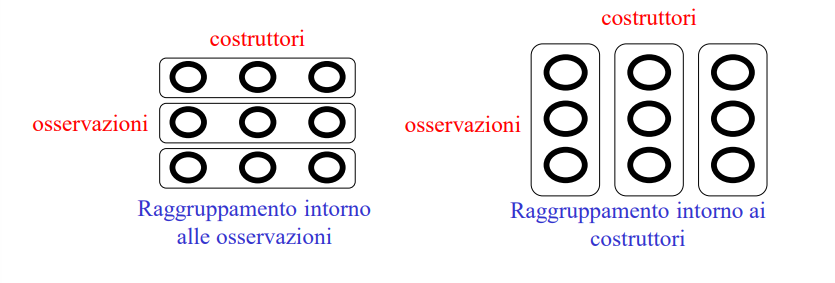
\includegraphics[width=0.8\linewidth]{assets/tipiastratticlassi} 
		\label{fig:etichetta}
	\end{figure}
	\\
	\subsubsection*{Vantaggi del tipo astratto}
	Nei linguaggi imperativi, i valori di un tipo astratto vengono trattati alla stregua dei valori di un tipo concreto, cioè sono cittadini di prima classe. Al contrario i valori rappresentati mediante oggetti sono trattati come cittadini di terza classe in quanto:
	\begin{itemize}
		\item una procedura non può restituire l'istanza di un generic package
		\item non è possibile creare dinamicamente degli oggetti (le istanze sono stabilite al momento della compilazione)
	\end{itemize}
	I tipi astratti son utili in tutti i paradigmi di programmazione, mentre gli oggetti, essendo variabili aggiornabili, si adattano bene solo a un paradigma di programmazione side-effecting.\\
	La notazione usata per chiamare un'operazione di un tipo astratto è più naturale perchè valori e variabili del tipo astratto sono argomenti espliciti.

	\subsubsection*{Svantaggi del tipo astratto}
	Il tipo astratto presenta scarsa estensibilità: l'aggiunta di un nuovo costruttore comporta dei cambiamenti intrusivi nelle implementazioni esistenti degli operatori. \\
	Ogni operatore dovrà essere opportunamente rivisto in modo da prevedere il trattamento di rappresentazioni ottenute con nuovi costruttori.

	\paragraph*{Esempio}
	Si vuole implementare il dato astratto \textit{geometricShape} la cui specifica algebrica è fornita di seguito:
	\begin{center}
	\begin{tabular}{|c|cc|}
	\hline
	\multirow{2}{*}{\textbf{Osservazioni}} & \multicolumn{2}{c|}{\textbf{Costruttore di g}}        \\ \cline{2-3} 
										   & \multicolumn{1}{c|}{square(x)}            & circle(x) \\ \hline
	area(g)                                & \multicolumn{1}{c|}{$x^2$} & $\pi*r*2$    \\ \hline
	\end{tabular}
	\end{center}
	\begin{verbatim}
		package geometric_shape_type
		type geometricShape is limited private;
			function square(x: in real) return geometricShape;
			function circle(x: in real) return geometricShape;
			function area(g: in geometricShape) return real;
		private
			type geometricShape is record
				shape: char;
				value: real;
			end;
		end geometric_shape_type; 

		package body geometric_shape_type
			function square(x: in real) return geometricShape is
				var g: geometricShape;
				begin
					g.shape := 's';
					g.value := x;
					return g;
				end;

			function circle(x: in real) return geometricShape is
				var g: geometricShape;
				begin
					g.shape := 'c';
					g.value := x;
					return g;
				end;

			function area(g: in geometricShape) return real is
				begin
					if g.shape = 's' then
						return g.value * g.value;
					else
						return 3.14159 * g.value * g.value;
					end if;
				end;
		end geometric_shape_type;
	\end{verbatim}
	Realizzando il dato astratto mediante classi si possono definire due moduli generici, uno per ogni forma geometrica (o costruttore):
	\begin{verbatim}
		generic package circle
			function area return real;
			procedure init(real);
		end circle;
		package body circle
			var raggio: real;
			procedure init(x: real) is
			begin
				raggio := x;
			end;

			function area return real is
			begin
				return 3.14159 * raggio * raggio;
			end;
		end circle;


		generic package square
			function area return real;
			procedure init(real);
		end square;
		package body square
			var lato: real;
			procedure init(x: real) is
			begin
				lato := x;
			end;

			function area return real is
			begin
				return lato * lato;
			end;
		end square;
	\end{verbatim}
	Per utilizzare una forma geometrica si deve istanziare una delle due classi e invocare il metodo \textit{init}.
	\vspace{\baselineskip} \\
	Se estendiamo la specifica del dato astratto in modo da considerare anche i rettangoli:
	\begin{center}
		\begin{tabular}{|c|ccc|}
			\hline
			\multirow{2}{*}{\textbf{Osservazioni}} & \multicolumn{3}{c|}{\textbf{Costruttore di g}}                                              \\ \cline{2-4} 
												   & \multicolumn{1}{c|}{square(x)}            & \multicolumn{1}{c|}{circle(x)} & rectangle(l,m) \\ \hline
			area(g)                                & \multicolumn{1}{c|}{x\textasciicircum{}2} & \multicolumn{1}{c|}{pi*r*2}    & l*m            \\ \hline
		\end{tabular}
	\end{center}
	Se abbiamo specificato un tipo astratto, siamo costretti a cambiare la rappresentazione in modo da memorizzare due valori ( pe ri due lati del rettangolo) e non uno:
	\begin{verbatim}
		type geometricShape is record
			shape: char;
			value, value2: real;
		end;
	\end{verbatim}
	Inoltre dobbiamo aggiungere l'opportuno costruttore e modificare anche la funzione area sempre supponendo di disporre del codice sorgente del modulo:
	\begin{verbatim}
		function rectangle(l,m: in real) return geometricShape is
			var g: geometricShape;
			begin
				g.shape := 'r';
				g.value := l;
				g.value2 := m;
				return g;
			end;

		function area(g: in geometricShape) return real is
			begin
				if g.shape = 's' then
					return g.value * g.value;
				elsif g.shape = 'c' then
					return 3.14159 * g.value * g.value;
				else
					return g.value * g.value2;
				end if;
			end;
	\end{verbatim}
	Diversamente, avendo realizzato il dato astratto mediante classi basta aggiungere un'altra classe:
	\begin{verbatim}
		generic package rectangle
			function area return real;
			procedure init(real, real);
		end rectangle;
		package body rectangle
			var lato1, lato2: real;
			procedure init(x, y: real) is
			begin
				lato1 := x;
				lato2 := y;
			end;

			function area return real is
			begin
				return lato1 * lato2;
			end;
		end rectangle;
	\end{verbatim}
	Per utilizzare un rettangolo si dovrà istanziare questa classe e invocare il metodo \textit{init}. \\
	Nella programmazione orientata ad oggetti, per evitare la riscrittura di codice comune ad altre classi già definite è possibile ricorrere ai meccanismo di ereditarietà tra le classi.

	\subsection{Astrazione generica}
	Il concetto di astrazione generica è fondamentale nel contesto della programmazione orientata agli oggetti. L'astrazione generica si applica non solo ai concetti di tipo e funzione, ma anche alle dichiarazioni di oggetti e classi. In particolare, essa suggerisce che è possibile definire astrazioni su dichiarazioni, dove la valutazione di una dichiarazione comporta la creazione di legami (bindings). \\
	Un'astrazione generica è un'astrazione su una dichiarazione, pertanto il corpo della dichiarazione di una astrazione generica è a sua volta una dichiarazione. La chiamata di un'astrazione generica è detta istanziazione e produce dei legami elaborando la dichiarazione contenuta nel corpo dell'astrazione generica.
	\vspace{\baselineskip} \\
	Un'astrazione generica può essere specificata come segue:
	\begin{align*}
	& \text{generic } I(FP_1, \ldots, FP_n) \text{ is } D
	\end{align*}
	dove:
	\begin{itemize}
		\item $I$ è un identificatore dell'astrazione generica,
		\item $FP_1, \ldots, FP_n$ sono i parametri formali, e
		\item $D$ è una dichiarazione che, quando elaborata, produrrà dei legami. $D$ funge da matrice dalla quale ricavare le dichiarazioni per istanziazione.
	\end{itemize}
	Una dichiarazione $D$ può essere di vario tipo, come ad esempio:
	\begin{itemize}
		\item La dichiarazione di un tipo,
		\item La dichiarazione di un modulo,
		\item La dichiarazione di una funzione,
		\item La dichiarazione di una procedura,
		\item \ldots
	\end{itemize}
	Per distinguere le diverse dichiarazioni ottenute per istanziazione, si può specificare un diverso identificatore, come nel seguente esempio:
	\begin{center}
		A istantiation of I;
	\end{center}
	Così, la seguente dichiarazione generica
	\begin{verbatim}
		generic typeRxR is
			type RxR is record
				x: real;
				y: real;
		end;
	\end{verbatim}
	potrà essere utilizzata come matrice per generare le dichiarazioni per i tipi Point2D e Complex:
	\begin{center}
	Point2D instantiation of typeRxR \\
	Complex instantiation of typeRxR
	\end{center}
	L'astrazione generica trova un ampio utilizzo nella dichiarazione di moduli dotati di stato locale. Mediante l'operazione di istanziazione si ottengono diverse copie dell'oggetto che differiscono solo per il nome dell'identificatore. \\
	In conclusione, l'astrazione generica di un oggetto corrisponde al concetto di classe.
	\vspace{\baselineskip} \\
	Il generic package di Ada è una esemplificazione di astrazione generica. L'espressione:
	\begin{center}
		package Stack is new Stack
	\end{center}
	è un esempio di istanziazione generica.
	\vspace{\baselineskip} \\
	Le astrazioni generiche, come qualsiasi altra astrazione possono essere parametrizzate.
	\paragraph*{Esempio}
	Definiamo la classe coda in ADA. La variabile \textit{items} è un array di caratteri. Al fine di svincolare la definizione di classe da particolari costanti legate all'applicazione si dota l'astrazione generica del parametro formale \textit{capacity}, che è utilizzato per dimensionare l'array. L'istanziazione deve consentire di specificare il parametro effettivo, che sarà un valore da associare al parametro formle. 
	In ADA l'istanziazione sarà specificata come segue:
	\begin{verbatim}
		package line_buffer is new queue_class(100);

		generic
			capacity: positive;
		package queue_class is
			procedure append(newitem: in character);
			procedure remove(olditem: out character);
		end queue_class;

		package body queue_class is
				items: array(1..capacity) of character;
				size, front, rear: integer range 0..capacity;

				procedure append(newitem: in character) is
				begin
					...
				end append;

				procedure remove(olditem: out character) is
				begin
					...
				end remove;
		end queue_class;
	\end{verbatim}
	In principio si può applicare l'astrazione generica a qualunque dichiarazione, incluso le procedure e le funzioni. \\
	Ad esempio, si potrebbe dichiarare una procedura T\_swap per scambiare dati di tipo T predefinito:
	\begin{verbatim}
		generic
		procedure T_swap(x, y: in out T);
		proceure T_swap(x, y: in out T) is
			temp: T;
			begin
				temp := x;
				x := y;
				y := temp;
			end T_swap;
	\end{verbatim}
	e ottenere diverse copie di essa per istanziazione:
	\begin{center}
		procedure swap1 is new T\_swap \\
		procedure swap2 is new T\_swap
	\end{center}
	In realtà è poco utile disporre di due funzioni identiche ma di nome diverso. Diversa sarebbe la situazione se potessimo dichiarare una generica procedure T\_swap che opera su fati di tipo T qualunque, e potessimo specificare il tipo al momento dell'istanziazione. Per ottenere questo risultato necessitiamo di un particolare classe di parametri, quelli di tipo.\\
	Per esempio:
	\begin{verbatim}
		generic
			type T is private;
		procedure T_swap(x, y: in out T);
		procedure T_swap(x, y: in out T) is
			temp: T;
			begin
				temp := x;
				x := y;
				y := temp;
		end T_swap;
	\end{verbatim}
	La clausola generic introduce un parametro di tipo e la dichiarazione che segue introduce la matrice di una procedura che scambia due dati di un tipo T generico. Le procedure effettive sono ottenute istanziando la procedura generica con i parametri di tipo effettivi da sostituire a T.\\
	Per esempio:
	\begin{center}
		procedute int\_swap is new T\_swap(integer);
		procedure str\_swap is new T\_swap(string);
	\end{center}
	Assumendo che i e j sono variabili di tipo integer e che s e t sono variabili di tipo string, allora:
	\begin{center}
		int\_swap(i, j);
		str\_swap(s, t);
	\end{center}
	è corretto, mentre:
	\begin{center}
		int\_swap(s, t);
		str\_swap(i, j);
		int\_swap(s, j);
	\end{center}
	è errato.
	\vspace{\baselineskip} \\
	In questo modo si è svincolato la definizione dello scambio di due elementi da un fattore marginale, come il tipo degli elementi da scambiare e si è garantito comunque il controllo statico dei tipo fra i parametri formali e parametri effettivi delle diverse procedure ottenute, e fra sorgente e destinazione di una assegnazione. \\
	L'uso dei parametri di tipo in astrazioni generiche offre un buon compromesso fra necessità di dover effettuare il controllo statico dei tipi e desiderio di definire componenti software riutilizzabili.
	\vspace{\baselineskip} \\
	I parametri di tipo possono essere utilizzati anche per definire astrazioni generiche di classi. \\
	Per esempio:
	\begin{verbatim}
		generic
			max: positive;
			type ITEM is private;
		package stack is
			procedure push(x: in ITEM);
			procedure pop;
			procedure top(x: out ITEM);
			function empty return boolean;
		end stack;
		package body stack is
			type stack is array(1..max) of ITEM;
			st: Table;
			top: integer range 0..max := 0;

			procedure push(x: in ITEM) is
			begin
				top := top + 1;
				st(top) := x;
			end push;

			procedure pop is
			begin
				top := top - 1;
			end pop;

			procedure top(x: out ITEM) is
			begin
				x := st(top);
			end top;

			function empty return boolean is
			begin
				return (top = 0);
			end empty;
	\end{verbatim}
	In questo caso per creare i singoli oggetti scriveremo:
	\begin{verbatim}
		declare
			package STACK_INT is new stack(100, integer);
			use STACK_INT;
			package STACK_REAL is new stack(100, real);
			use STACK_REAL;
			A: REAL; B: INTEGER;
		begin
			push(1);
			push(2.0);
			top(A);
			top(B);
		end;
	\end{verbatim}
	Si osservi che non è necessario utilizzare la notazione puntata:
	\begin{center}
		STACK\_INT.push(1);
		STACK\_REAL.push(2.0);
	\end{center}
	in quanto push e top sono differeniate dal contesto (tipo di parametro effettivo passato). Questo è un caso di \textit{overloading} come si chiarirà meglio in seguito.
	\vspace{\baselineskip} \\
	L'astrazione generica è quindi di supporto all'astrazione dati, in quanto permette di definire delle classi che sono invarianti ad alcuni tipi di dati neccessari per definirle. \\
	Inoltre, essa, mediante i parametri di tipo, è applicabile a tipi astratti che possono essere così ugualmente svincolati dalla necessità di specificare il tipo degli elementi sui quali operare.

	\paragraph*{Esempio}
	Si consideri il problema di definire dei tipi astratti per una applicazione che usa:
	\begin{enumerate}
		\item stack di interi
		\item stack di reali
		\item stack di un tipo astratto \textit{point3d} utilizzato per rappresentare i punti in uno spazio tridimensionale
	\end{enumerate}
	Una alternativa sarebbe quella di scrivere una definizione separata per ciascuno dei tre tipo. Così facendo, però, si produrrebbe codice duplicato in quanto plausibilmente simile per tutte le definizioni (differisce solo nelle parti in cui si fa riferimento ai singoli elementi dello stack). Inoltre ci sarebbe uno sforzo di programmazione ridondante accompagnato da una manutenzione complicata poichè le modifiche, come l'aggiunta di un nuovo operatore, dovrebbero essere effettuate in tutte le definizioni. \\
	Allora si potrebbe ricorrere alla separazione delle proprietà di uno stack dalle proprietà dei suoi elementi mediante i parametri di tipo:
	\begin{verbatim}
		generic
			max: positive;
			type ITEM is private;
		package stacks is
			type stack is limited private;
			procedure push(s: in out stack; x: in ITEM);
			procedure pop(s: in out stack, x: out ITEM);
		private
			type stack is record
				st: array(1..max) of ITEM;
				top: integer range 0..max := 0;
			end record;
		end stacks;

		package body stacks is
			procedure push(s: in out stack; x: in ITEM) is
			begin
				s.top := s.top + 1;
				s.st(s.top) := x;
			end push;

			procedure pop(s: in out stack; x: out ITEM) is
			begin
				x := s.st(s.top);
				s.top := s.top - 1;
			end pop;
		end stacks;
	\end{verbatim}
	In questo modo di è definito un tipo astratto generico stack. \\
	I diversi stack richiesti sono ottenuti per istanziazione:
	\begin{verbatim}
		declare
			package my_stack is new stacks(100, real);
			use my_stack;
			x: stack; y: real;
		begin
			push(x, 1.0);
			pop(x, y);
		end;
	\end{verbatim}
	Se un'astrazione è parametrizzata rispetto a un valore, possiamo usare l'argomento valore anche se non sappiamo nulla al di fuori del suo tipo. Analogamente se un'astrazione è parametrizzata rispetto a una variabile, possiamo ispezionare e aggiornare la variabile anche se non sappiamo nulla al di fuori del suo tipo. \\
	Ma quando si parametrizza rispetto al tipo la situazione cambi. Nell'esempio di T\_swap avevamo le seguenti assegnazioni:
	\begin{center}
		temp := x; \\
		x := y; \\
		y := temp;
	\end{center}
	ma chi garantisce che il tipo T supporti l'operatore di assegnazione? \\
	In ADA l'espressione
	\begin{center}
		type T is private;
	\end{center}
	sottintende che l'assegnazione e i predicati $=$ e $\neq$ sono operazioni valide per il tipo effettivo denotato da T. Per questo tutti gli esempi visti finora non hanno generato errori. \\
	Se T fosse stato definito come limited private avremmo dovuto specificare un'operazione di assegnazione e i predicati di uguaglianza e disuguaglianza.

	\subsection{Esercizi}
	\subsubsection*{Esercizio 1}
	Fornire una realizzazione di una tipo astratto Dizionario in Ada (si ipotizzi che Chiave e Valore siano di tipo Intero e Carattere). Per tale esercizio considerare la specifica sintattica fornita nel seguito:
	\begin{itemize}
		\item creaDizionario()$\rightarrow$Dizionario
		\item aggiungi(Dizionario,Chiave,Valore)$\rightarrow$Dizionario
		\item leggi(Dizionario,Chiave)$\rightarrow$Valore
		\item cancella(Dizionario,Chiave)$\rightarrow$Dizionario
		\item uguale(Dizionario,Dizionario)$\rightarrow$Booleano
	\end{itemize}
	Mostrare l'uso del tipo scritto. Commentare il codice scritto.
	\paragraph*{Soluzione}
	\begin{verbatim}
		package Dizionario
		begin
		Type Dizionario is limited private;
			procedure aggiungi(d: inout Dizionario, c: in Integer, v: in Character);
			function leggi(d: in Dizionario, c: in Integer) return Character;
			procedure cancella(d:inout Dizionario, c: in Integer);
			function uguale( d1: in Dizionario, d2: in Dizionario) return Boolean;
		private:
			constant max: Positive=200;
			type Dizionario is record
				chiavi: array [1..max] of Integer;
				valori: array[1..max] of Character;
				top: Positive=0;
			end 
		end

		package body Dizionario
		begin
			function cerca(d: in Dizionario, c: in Integer) return Positive
			var i: Positive
			begin
				if D.top > 0 then
					for i=1 to D.top loop
						if c= D.chiavi[i] then
							return i;
				return 0;
			end

			procedura aggiungi(d: inout Dizionario, c: in Integer, v: in Character)
			begin
				if d.top < max then
					if cerca(D,c) =0 begin
						D.top=D.top+1;
						D.chiavi[D.top]=c;
						D.valori[D.top]=v
					end
				else raise Exception;
			end

			function leggi(d: in Dizionario, c: in Integer) return Character
				var x:Positive
				begin
					x=cerca(D,c);
					if x=0 then raise Exception
					else return D.valori[x];
				end

			procedure cancella(d:inout Dizionario, c: in Integer)
				var x, i:Positive;
				begin
					x=cerca(D,c);
					if x=0 then raise Exception;
					else
					begin
						for i= x to D.top-1 loop
						begin
							D.chiavi[i]=D.chiavi[i+1]
							D.valori[i]=D.valori[i+1];
						end
						D.top=D.top-1;
					end
				end

			function uguale( d1: in Dizionario, d2: in Dizionario) return Boolean
				var i:Positive
				begin
					if d1.top= d2.top then
						for i=1 to D1.top loop
						begin
							x=cerca(d2,d1.chiavi[i])
							if x=0 then return false;
							else
								if d2.valori[x] not = d1.valori[i] then return false; 
						end
						return true;
					else return false;
				end
		end

		...
		With Dizionario; use Dizionario;
		var D1,D2:Dizionario;
		var x:Positive:
		inserisci(D1,1,'a')
		inserisci(D1,2,'b')
		inserisci(D2,1,'c')
	\end{verbatim}
	\newpage
	\subsubsection*{Esercizio 2}
	Fornire una realizzazione di una tipo astratto Dizionario in Ada (si ipotizzi che Chiave e Valore siano di tipo Intero e Carattere). Per tale esercizio considerare la specifica sintattica fornita nel seguito:
	\begin{itemize}
		\item creaDizionario()$\rightarrow$Dizionario
		\item aggiungi(Dizionario,Chiave,Valore)$\rightarrow$Dizionario
		\item leggi(Dizionario,Chiave)$\rightarrow$Valore
		\item cancella(Dizionario,Chiave)$\rightarrow$Dizionario
		\item uguale(Dizionario,Dizionario)$\rightarrow$Booleano
	\end{itemize}
	Mostrare l'uso della classe scritta. Commentare il codice scritto.
	\paragraph*{Soluzione}
	\begin{verbatim}
		Generic
		max:positive
		Package Dizionario
		Begin
			procedure aggiungi( c: in Integer, v:In Character);
			function leggi(c:in Integer) return Characger;
			procedure cancella(c: in Integer);
		end

		package body Dizionario
		begin
			var top: Positive = 0;
			var chiavi: array [1…max] of Integer;
			var valori: array [1..max] of Character;

			//funzione creata internamente
			function cerca(c: in Integer) return Positive
			var i: Positive
			begin
				if top > 0 then
					for i = 1 to top loop
						if c = chiavi[i] then
							return i;
				return 0;
			end

			procedura aggiungi(c: in Integer, v: in Character)
			begin
				if top < max then
					if cerca(c) = 0 begin
						top = top + 1;
						chiavi[top] = c;
						valori[top] = v
					end
				else raise Exception;
			end

			function leggi(c: in Integer) return Character
			var x: Positive
			begin
				x = cerca(c);
				if x = 0 then raise Exception
				else return valori[x];
			end

			procedure cancella(c: in Integer)
			var x, i:Positive;
			begin
				x = cerca(c);
				if x = 0 then raise Exception;
				else
				begin
					for i = x to top-1 loop
					begin
						chiavi[i] = chiavi[i+1]
						valori[i] = valori[i+1];
					end
					top = top - 1;
				end
			end
		end

		..
		with Dizionario;
		package d1 is new Dizionario(3);
		package d2 is new Dizionario(300);
		with d1; use d1;
		with d2, use d2;
		d1.aggiungi(1,'a');
	\end{verbatim}
	%%aggiungi commenti esercizi e finisci gli altri

	\newpage
	\section{Paradigma Object Oriented}
	Nella programmazione imperativa, gli oggetti possono essere definiti, ma il loro utilizzo non è rigidamente imposto e dipende dall'autodisciplina dei programmatori. Inoltre, gli oggetti non godono dello status di cittadini di prima classe. Ciò significa che non hanno la stessa importanza e trattamento dei dati primitivi come interi o stringhe.
	\vspace{\baselineskip} \\
	D'altra parte, nel paradigma orientato agli oggetti, c'è una trasformazione significativa. Gli oggetti diventano cittadini di prima classe, il che significa che hanno un ruolo centrale e sono trattati su un piano paritario con altri elementi del linguaggio. Questa trasformazione può essere vista come una rivoluzione poiché gli oggetti assumono un ruolo fondamentale nella progettazione e nella programmazione. 
	\vspace{\baselineskip} \\
	Principi come l'information hiding e l'incapsulamento diventano cardini del paradigma orientato agli oggetti, permettendo una migliore organizzazione, manutenzione e scalabilità del codice. Inoltre, l'orientamento agli oggetti incoraggia una maggiore modularità e riusabilità del codice attraverso concetti come l'ereditarietà e il polimorfismo, consentendo agli sviluppatori di costruire sistemi complessi in modo più efficiente e intuitivo.
	
	\subsection{Oggetti}
	Gli oggetti sono strutture dati complesse che combinano sia lo stato, che rappresenta le informazioni associate all'oggetto, sia il comportamento, che definisce le azioni che l'oggetto può eseguire. 
	\vspace{\baselineskip}\\
	Lo stato di un oggetto è tipicamente identificato dal contenuto di una specifica area di memoria, mentre il comportamento è definito da una collezione di procedure e funzioni chiamate metodi, che operano sullo stato dell'oggetto stesso.
	\vspace{\baselineskip}\\
	Da una prospettiva di progetto, gli oggetti sono utilizzati per modellare le entità presenti nel dominio dell'applicazione, consentendo agli sviluppatori di creare astrazioni efficaci e rappresentazioni del mondo reale all'interno del software. Questo approccio favorisce una progettazione modulare, manutenibile e scalabile, in cui gli oggetti possono essere istanziati, manipolati e interagiti tra loro per creare sistemi complessi e funzionali. Inoltre, l'incapsulamento degli stati e dei comportamenti all'interno degli oggetti favorisce la sicurezza e l'integrità del sistema, poiché limita l'accesso diretto ai dati e alle operazioni, consentendo un migliore controllo e gestione delle interazioni tra le varie parti del software.
	\paragraph{Esempio}
	In un gioco elettronico che us una palla, si può penare alla palla come un oggetto dotato di uno:
	\begin{itemize}
		\item \textbf{Stato}: posizione, velocità, colore, dimensione, ecc.
		\item \textbf{Comportamento}: muoversi, rimbalzare, cambiare colore, cambiare dimensione, apparire e sparire, ecc.
	\end{itemize}
	Le variabili e i metodi definiti nell'oggetto \textit{palla} stabiliscono lo stato e il comportamento che sono rilevanti all'uso della palla nel gioco elettronico.

	\subsection{Identificatore di oggetto}
	Un oggetto ha la sua \textbf{identità}, cioè è riconoscibile indipendentemente dal suo stato corrente. Per questo ogni oggetto ha un \textbf{identificatore di oggetto} (object identifier, OID) che lo identifica univocamente. In alcuni contesti gli OID sono anche detti \textbf{riferimenti} (references).
	Un identificatore di oggetto è immutabile, cioè non può essere modificato da una qualche opzione di programmazione. Cambiare l'OID di un oggetto equivale alla cancellazione dell'oggetto e alla creazione di un altro oggetto con lo stesso stato.\\\\
	Normalmente gli OID sono assegnati in modo automatico agli oggetti, sicchè non hanno un significato nel mondo reale.
	In molti ambienti di programmazione object-oriented, l'OID corrisponde all'indirizzo dell'area di memoria che conserva lo stato dell'oggetto.
	Quasi mai il programmatore utilizza esplicitamente i riferimenti. Generalmente questi vengono legati a delle varibili e si fa riferimento agli oggetti mediante gli identificatori di variabile. \\\\
	Variabili distinte possono riferirsi al medesimo oggetto. In questo caso si hanno degli alias. La presenza di alias non significa che un oggetto non è identificato univocamente, ma semplicemente che diversi identificatori di variabile sono stati legati al medesimo riferimento di oggetto. \\\\
	Lo stato di un oggetto può anche contenere il riferimento ad un altro oggetto. Si dice che un oggetto punta ad un altro. Il puntamento è asimmetrico. La simmetria si ottiene mediante la reciprocità di puntamento.

	\subsection{Classi}
	Una \textbf{classe} è la descrizione di una famiglia di oggetti che condividono la stessa struttura (gli attributi) e il medesimo comportamento (operazioni). \\
	Nella programmazione OO \textbf{ogni oggetto è un'istanza di una classe}, cioè un oggetto non può essere ottenuto se non si definisce la sua classe di appartenenza. Analogamente nella modellazione OO le istanze esistono in quanto ci sono le loro astrazioni.\\
	\textbf{Idealmente una classe è una realizzazione di un dato astratto}. Questo significa che i dettagli della realizzazione sono normalmente nascosti. Ogni classe ha una doppia componente:
	\begin{enumerate}
		\item \textbf{Componente statica}, i dati, costituita da campi o \textbf{attributi} dotati di nome, che contengono un valore. I campi caratterizzano lo stato degli oggetti durante l'esecuzione del programma.\\
	\end{enumerate}
	Gli attributi si distinguono in base al loro ambito d'azione (\textbf{scope}):
	\begin{itemize}
		\item \textbf{Attributi d'istanza}: sono associati ad una istanza e hanno un tempo di vita pari a quello dell'istanza alla quale sono associati.
		\item \textbf{Attributi di classe}: sono associati alla classe e non alle istanze. Sono condivisi da tutte le istanze della classe e sono definiti una sola volta. Il loro tempo di vita è lo stesso della classe.
	\end{itemize}
	Gli attributi d'istanza contribuiscono a caratterizzare lo stato di ogni singolo oggetto, mentre gli attributi di classe contribuiscono a definire il fattore comune allo stato di tutti gli oggetti di una classe.
	\begin{enumerate}[start=2]
		\item \textbf{Componente dinamica}, i \textbf{metodi} (operazioni), che caratterizzano il comportamento comune degli oggetti appartenenti alla classe, cioè i servizi che possono essere richiesti a un oggetto di una classe durante l'esecuzione del programma. I metodi manipolano gli \textbf{attributi}.
	\end{enumerate}
	I metodi possono essere classificati:
	\begin{enumerate}
		\item \textbf{Metodi costruttori}: sono invocati per creare (istanziare) gli oggetti e inizializzarli.
		\item \textbf{Metodi distruttori}: sono invocati per distruggere gli oggetti rimuovendoli dalla memoria.
		\item \textbf{Metodi di accesso}: restituiscono astrazioni significative dello stato di un oggetto.
		\item \textbf{Metodi di trasformazione}: modificano lo stato di un oggetto.
	\end{enumerate}
	I metodi di accetto e trasformazioni possono essere distinti in:
	\begin{enumerate}
		\item \textbf{Metodi di istanza}: operano su almeno un attributo di istanza, pertanto possono essere invocati solo specificando l'istanza.
		\item \textbf{Metodi di classe}: operano esclusivamente su attributi di classe, pertanto possono essere invocati specificando la classe. Si possono invocare metodi di classe anche quando non è stato creato alcun oggetto per quella classe.
	\end{enumerate}
	L'invocazione di un metodo di classe può avvenire anche specificando un oggetto (e non la classe), tuttavia ciò è sconsigliato perchè non evidenzia il fatto che si manipolano solo attributi di classe. \\
	Non è possibile invocare un metodo di istanza sulla classe.

	\subsection{UML}
	\textbf{UML}, acronimo di Unified Modeling Language, è un \textbf{linguaggio visuale} ampiamente utilizzato nell'ambito dello sviluppo software per definire, progettare, realizzare e documentare sistemi orientati agli oggetti. Questo linguaggio fornisce una serie di strumenti e convenzioni grafiche che consentono agli sviluppatori di rappresentare in modo chiaro e conciso i concetti e le relazioni all'interno di un sistema.
	\vspace{\baselineskip} \\
	Uno dei principali vantaggi di UML è la sua \textbf{universalità}: può essere impiegato per modellare una vasta gamma di sistemi, indipendentemente dalla loro architettura, tecnologie utilizzate o tipologia applicativa. Questo rende UML uno strumento flessibile e adattabile alle esigenze di progettazione di diversi contesti, che vanno dai sistemi gestionali ai sistemi real-time e oltre.
	\vspace{\baselineskip} \\
	Tra le sue funzionalità principali, UML supporta attivamente il processo di progettazione di nuovi sistemi, consentendo agli sviluppatori di visualizzare e analizzare in dettaglio i requisiti, le interazioni e le relazioni tra le varie componenti del sistema. Inoltre, UML è prezioso anche per la documentazione dei sistemi esistenti, offrendo un mezzo efficace per rappresentare e comunicare l'architettura e il funzionamento di un'applicazione software agli stakeholder.

	\subsubsection{Oggetto}
	In UML un \textbf{oggetto (o istanza)} è graficamente rappresentato in questo modo:
	\begin{center}
		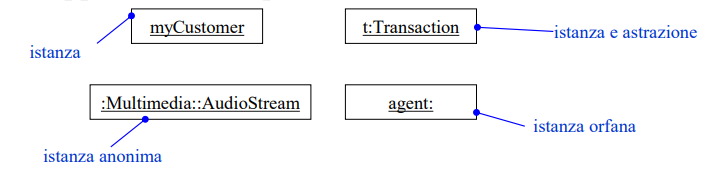
\includegraphics[scale=0.8]{assets/uml_oggetto.png}
	\end{center}
	E' possibile indicare:
	\begin{itemize}
		\item solo il nome (OID) dell'istanza
		\item nome dell'istanza e della astrazione (la classe) a cui appartiene
		\item solo il nome dell'astrazione, qualora non si conosca a priori il nome dell'istanza
		\item un'istanza orfana, se non si conosce a priori la sua astrazione
	\end{itemize}

	\subsubsection{Stato}
	Lo \textbf{stato} di un oggetto può essere rappresentato in modo astratto:
	\begin{center}
		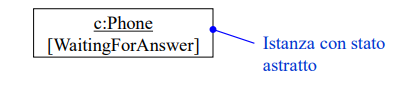
\includegraphics[scale=0.8]{assets/uml_stato.png}
	\end{center}
	oppure indicando esplicitamente i valori assunti dagli attributi dell'oggetto:
	\begin{center}
		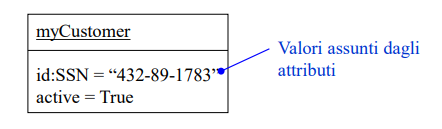
\includegraphics[scale=0.8]{assets/uml_stato_esplicito.png}
	\end{center}

	\subsubsection{Attributi}
	Graficamente gli attributi sono indicati sotto il nome della classe e si può specificare l'insieme dei valori assunti (oggetti di una classe) e una eventuale inizializzazione.
	\begin{center}
		\begin{tabular}{|l|}
		\hline
		\multicolumn{1}{|c|}{Rettangolo}                                       \\ \hline
		\begin{tabular}[c]{@{}l@{}}base: real = 10\\ altezza: real\end{tabular} \\ \hline
		\end{tabular}
	\end{center}
	Un attributo di classe (detto \textbf{statico} in UML) è indicato come sottolineato:
	\begin{center}
		\begin{tabular}{|l|}
		\hline
		\multicolumn{1}{|c|}{Rettangolo}                                                                  \\ \hline
		\begin{tabular}[c]{@{}l@{}}\underline{numRettangoli: integer=0}\\ base: real = 10\\ altezza:real\end{tabular} \\ \hline
		\end{tabular}
	\end{center}
	L'attributo \underline{numRettangoli} indica il numero di oggetti della classe Rettangoli che sono stati istanziati. E' un attributo statico (o di classe) in quanto condiviso da tutte le istanze della classe Rettangoli. \\	
	Esso è inizializzato a 0 e verosimilmente sarà incrementato dai costruttori della classe Rettangoli, mentre sarà decrementato dai distruttori. \\
	\vspace{\baselineskip} \\
	Gli attributi \textbf{derivati} sono quelli che possono essere calcolati partendo da attributi. UML prevede una rappresentazione specifica mediante una /.
	\begin{center}
		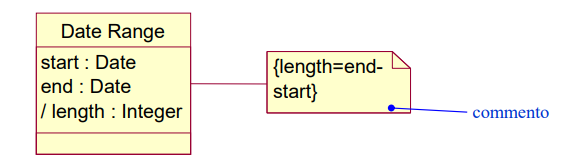
\includegraphics[scale=0.8]{assets/uml_attr_derivati.png}
	\end{center}
	Il commento sulla destra fa parte della notazione standard UML e in questo caso è utilizzato per indicare come si calcola l'attributo derivato length. \\
	I commenti possono essere aggiunti a qualunque elemento della notazione UML.

	\subsubsection{Operazioni}
	In UML le operazioni sono indicate graficamente in una sezione al di sotto degli attributi.
	\begin{center}
		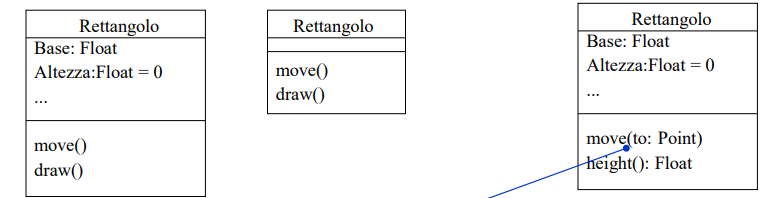
\includegraphics[scale=0.6]{assets/uml_operazioni.png}
	\end{center}
	Di una operazione si può specificare la segnatura.

	\subsubsection{Classe}
	La \textbf{classe} può essere rappresentata graficamente mediante un rettangolo:
	\begin{center}
		\begin{tabular}{|c|}
		\hline
		\multirow{2}{*}{\textbf{Cliente}} \\
									\\ \hline
		\end{tabular}
	\end{center}
	Ogni classe deve avere un nome che lo contraddistingue dalle altre. Questo può essere semplice o indicare un percorso.
	\begin{center}
		\begin{tabular}{|c|}
		\hline
		\multirow{2}{*}{\textbf{java.awt.Rectangle}} \\
										  \\ \hline
		\end{tabular}
	\end{center}
	Una classe può essere rappresentata a diversi livelli di dettaglio:
	\begin{itemize}
		\item specificandone solo il nome
		\begin{center}
			\begin{tabular}{|c|}
				\hline
				\multirow{2}{*}{\textbf{Cliente}} \\
											\\ \hline
				\end{tabular}
		\end{center}
		\item specificandone gli attributi e i metodi
		\begin{center}
			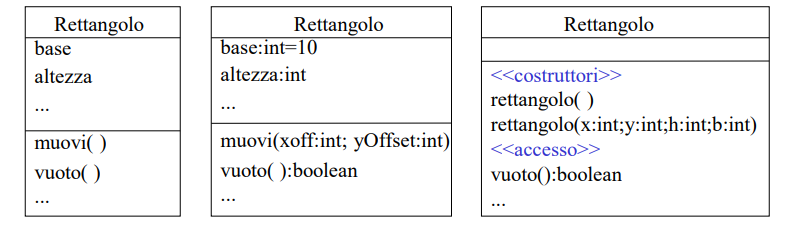
\includegraphics[scale=0.6]{assets/uml_classi_attr_met.png}
		\end{center}
	\end{itemize}
	I diversi livelli di dettaglio consentono a chi progetta/modella di attribuire maggiore o minore importanza a determinati fattori a seconda della vista del sistema che si sta considerando.

	\subsubsection{Stereotipi}
	Nel precedente esempio si è fatto uso della notazione \textbf{$<<$costruttori$>>$} e \textbf{$<<$accesso$>>$}. Questi sono due tipici esempi di \textbf{stereotipi}.
	\vspace{\baselineskip} \\
	Gli stereotipo sono dei tipici \textit{meccanismi di estensibilità} del vocabolario UML e permettono di creare nuovi blocchi per la costruzione dei modelli, derivandoli da blocchi già esistenti ma rendendoli specifici per il particolare dominio.
	\vspace{\baselineskip} \\
	Nel precedente esempio è stato esteso il blocco \textit{operazioni} in modo da poter distinguere le diverse tipologie di operazioni.
	\vspace{\baselineskip} \\
	Gli stereotipi sono identificabili perchè racchiusi da una coppia di caporali (\textit{guillemet}, in inglese) \textbf{$<<$ $>>$}. \\
	Sono già previsti diversi stereotipi in UML.

	\subsubsection{Visibilità}
	Gli attributi e i metodi di una classe possono avere diversi livelli di \textbf{visibilità}. Un elemento (attributo o metodo) ha visibilita:
	\begin{itemize}
		\item \textbf{public}: l'elemento può essere visto, utilizzato e/o invocato da altre classi.
		\item \textbf{protected}: l'elemento è visibile all'interno del package e all'esterno solo ai discendenti della classe di appartenenza.
		\item \textbf{private}: l'elemento è accessibile solo dalla classe di appartenenza.
		\item \textbf{package}: l'elemento è visibile all'interno del package che contiene la classe in cui l'elemento è definito.
	\end{itemize}
	Ad esempio, un metodo pubblico può essere invocato da qualunque punto del codice (purchè la classe sia \textit{importata} in qualche modo), mentre un metodo privato può essere invocato solo da altri metodi della stessa classe.
	\vspace{\baselineskip} \\
	UML consente di specificare i livelli di visibilità di attributi e metodi utilizzando la seguente notazione:
	\begin{itemize}
		\item \textbf{public}: elemento preceduto da un $+$.
		\item \textbf{protected}: elemento preceduto da un \#.
		\item \textbf{private}: elemento preceduto da un $-$.
		\item \textbf{package}: elemento preceduto da un \textasciitilde.
	\end{itemize}
	\begin{center}
		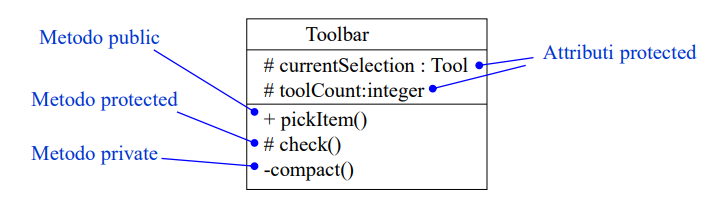
\includegraphics[scale=0.6]{assets/uml_visibilita.png}
	\end{center}

	\subsubsection{Molteplicità di classe}
	Con il termine \textbf{molteplicità di classe} si intende il numero di istanze di una classe che essa può avere. Generalmente non si pone un limite, tuttavia in alcuni casi è necessario indicare che la classe può avere una sola istanza (\textbf{classe singoletto}, \textit{singleton class}) o comunque un numero ben definito di istanze.
	\vspace{\baselineskip} \\
	UML impone che tale valore sia indicato in alto a destra nell'icona raprresentante la classe.
	\begin{center}
		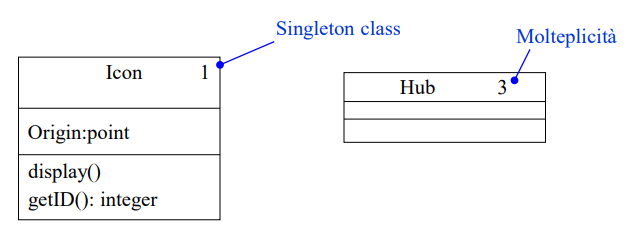
\includegraphics[scale=0.6]{assets/uml_molteplicita_classi.png}
	\end{center}
	Per realizzare una classe singoletto si rendono privati i costruttori della classe e dotando la classe di un attributo statico che è inizializzato all'unico oggetto di quella classe. Nessun metodo della classe singoletto invocherà il costruttore, nè potrà farlo un utente della classe. Inoltre può essere utile disporre di un metodo di classe che restituisce l'unica istanza memorizzata nella stessa classe singoletto.

	\subsubsection{Molteplicità di attributo}
	E' possibilità indicare la molteplicità anche per gli attributi, subito dopo il loro nome.
	\begin{center}
		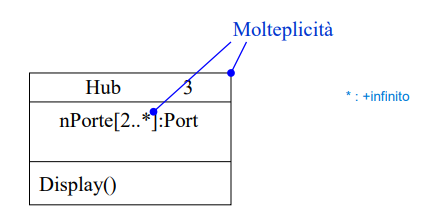
\includegraphics[scale=0.6]{assets/uml_molteplicita_attr.png}
	\end{center}

	\subsubsection{Schema di definizione di un attributo}
	Si è visto come è possibile specificare in UML le varie caratteristiche degli attributi di una classe. A riepilogo, mostriamo lo schema generale per la definizione di un attributo:
	\begin{center}
		[visibilità] nome [molteplicità] [: tipo] [= valore iniziale] [{proprietà}]
	\end{center}
	dove [..] significa opzionale.
	\vspace{\baselineskip} \\
	Alcuni esempi di definizioni lecite di attributo sono:
	\begin{center}
		\begin{tabular}{ll}
		\begin{tabular}[c]{@{}l@{}}- origine\\ - + origine\\ - origine: point\\ - testa: *elemento\\ - nome {[}0..1{]}: String\\ - origine: Point = (0,0)\\ - id: Integer \{frozen\}\end{tabular} & \begin{tabular}[c]{@{}l@{}}solo il nome\\ visibilità e nome\\ nome e tipo\\ nome e tipo complesso\\ nome, molteplicità e tipo\\ nome, tipo e valore iniziale\\ nome, tipo e proprietà\end{tabular}
		\end{tabular}
	\end{center}
	Focalizziamo l'attenzione sull'ultimo degli esempi:
	\begin{center}
		\begin{tabular}{ll}
		\begin{tabular}[c]{@{}l@{}}- id: Integer \{frozen\}\end{tabular} & \begin{tabular}[c]{@{}l@{}}nome, tipo e proprietà\end{tabular}
		\end{tabular}
	\end{center}
	In UML esistono tre \textbf{proprietà} che possono essere utilizzate con gli attributi:
	\begin{itemize}
		\item \textbf{changeable}: non vi sono restrizioni sulla modificabilità dell'attributo.
		\item \textbf{frozen}: l'attributo non può essere modificato dopo che l'oggetto è stato inizializzato.
		\item \textbf{addOnly}: per gli attributi con molteplicità maggiore di uno, i valori possono essere aggiunti, ma una volta creati, non possono più essere rimossi o modificati.
	\end{itemize}
	Nel caso in cui la proprietà non viene specificata si sottintende che assume valore \textit{changeable}.

	\subsubsection{Schema di definizione di una operazione}
	Prima di procedere con la definizione dello schema per la definizione di un'operazione, è necessario sottolineare che UML distingue tra operazione e metodo:
	\begin{itemize}
		\item \textbf{operazione}: è un servizio che può essere richiesto alla classe\
		\item \textbf{metodo}: è un'implementazione concreta del servizio.
	\end{itemize}
	Infatti, possono anche esistere diversi metodi per la stessa operazione nei diversi livelli della gerarchia delle classi.
	\vspace{\baselineskip} \\
	Lo schema generale per la definizione di una operazione è il seguente:
	\begin{center}
		[visibilità] nome [(parametri)] [: valore di ritorno] [{proprietà}]
	\end{center}
	Alcuni esempi di definizioni lecite di operazioni sono:
	\begin{center}
		\begin{tabular}{ll}
		\begin{tabular}[c]{@{}l@{}}- visualizza\\ - + visualizza\\ - set(n: nome, s: String)\\ - getID(): Integer\\ - riparti() \{guarded\}\end{tabular} & \begin{tabular}[c]{@{}l@{}}solo il nome\\ visibilità e nome\\ nome e parametri\\ nome e tipo del dato restituito\\ nome e proprietà\end{tabular}
		\end{tabular}
	\end{center}
	Ogni parametro riportato nella segnatura prende la forma:
	\begin{center}
		[direzione] nome: tipo [= valore iniziale]
	\end{center}
	La \textbf{direzione} può assumere uno dei seguenti valori:
	\begin{itemize}
		\item \textbf{in}: parametro di input, non può essere modificato
		\item \textbf{out}: parametro di output, può essere modificato per comunicare un'informazione al chiamante.
		\item \textbf{inout}: parametro di input che comunque può essere modificato.
	\end{itemize}
	UML fornisce diverse proprietà predefinite per le operazioni:
	\begin{itemize}
		\item \textbf{isQuery}: l'esecuzione dell'operazione lascia lo stato del sistema immutato, un'operazione con tale proprietà è quindi priva di \textit{side-effect}.
		\item \textbf{leaf}: l'operazione non può essere più specializzata (overriding) nelle sottoclassi (vedi \textit{final} in Java).
		\item \textbf{sequential}: i chiamanti (callers) di questo oggetto devono coordinarsi affinchè solo uno alla volta richieda il servizio. Nel caso di sovrapposizione la semantica e l'integrità dell'oggetto non sono garantite.
		\item \textbf{guarded}: simile al caso precedente, in ogni istante un solo chiamante può usufruire del servizio, tuttavia, in questo caso, la sequenzialità del servizio è gestita dalla classe proprietaria del servizio stesso (vedi \textit{synchronized} in Java).
		\item \textbf{concurrent}: la semantica e l'integrità dell'oggetto sono garantite anche in caso di chiamate multiple.
	\end{itemize}

	\subsubsection{Classi attive}
	Le ultime tre proprietà sono rilevanti solo in classi \textbf{attive}, cioè in classi i cui \textbf{oggetti} sono \textbf{attivi}.
	\vspace{\baselineskip} \\
	Un oggetto è attivo se esso ha un thread e può far partire un thread concorrente.
	\\\\
	Una classe attiva è simile ad una classe con l'eccezione che le sue istanze rappresentano elementi il cui comportamento è concorrente con gli altri. \\
	Essa è mostrata con bordi raddoppiati:
	\begin{center}
		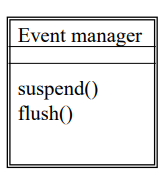
\includegraphics[scale=0.7]{assets/uml_classi_attive.png}
	\end{center}

	\subsubsection{Classi template}
	Una \textbf{classe template} definisce una famiglia di classi parametrizzate (con parametro di tipo). Non è possibile usare direttamente una classe template. E' necessario prima specificare il tipo (operazione di istanziazione). \\
	In Java, una classe template corrsponde a una classe generica.
	\vspace{\baselineskip} \\
	Esempio:
	\begin{center}
		public class ArrayList$<$E$>$
	\end{center}
	Notazione UML:
	\begin{center}
		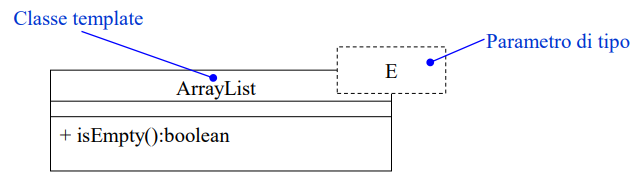
\includegraphics[scale=0.7]{assets/uml_classe_template.png}
	\end{center}
	Si potrebbe voler istanziare questo template per creare una lista di clienti.
	\begin{center}
		ArrayList$<$Customer$>$ elenco\_clienti;
	\end{center}
	L'istanziazione di una classe template può essere effettuata in due modi:
	\begin{enumerate}
		\item Implicitamente, dichiarando una classe il cui nome esplicita i parametri.
		\item Esplicitamente, mediante una dipendenza stereotipata $<<$bind$>>$.
	\end{enumerate}
	\begin{center}
		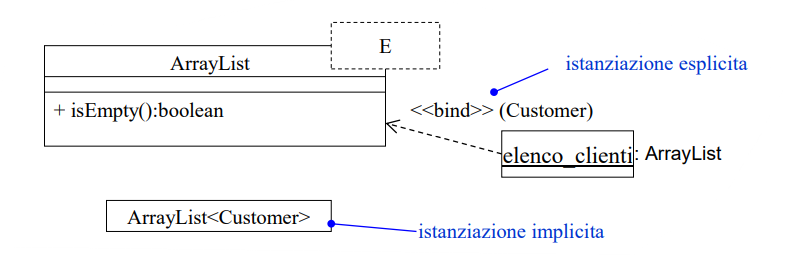
\includegraphics[scale=0.7]{assets/uml_classe_template_2.png}
	\end{center}

	\subsubsection{Individuazione delle responsabilità}
	In una buona modellazione Object-Oriented di un sistema sofware è necessario stabilire le responsabilità da attribuire a ciascuna classe individuata.
	\vspace{\baselineskip} \\
	UML consente di modellare le responsabilità in due modi:
	\begin{itemize}
		\item specificandole all'interno della classe:
		\begin{center}
			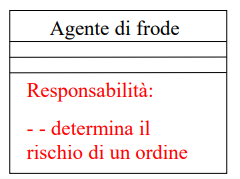
\includegraphics[scale=0.7]{assets/responsabilita_interna.png}
		\end{center}
		\item utilizzando le note:
		\begin{center}
			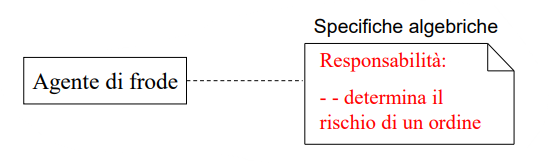
\includegraphics[scale=0.7]{assets/responsabilita_note.png}
		\end{center}
	\end{itemize}

	\subsubsection{Relazione Instance-of}
	Fra un oggetto e una classe sussiste una relazione \textbf{instance of} che specifica che un oggetto è una istanza di una classe.
	\vspace{\baselineskip} \\
	In UML questa relazione è resa con lo stereotipo $<<$instance of$>>$.
	\vspace{\baselineskip} \\
	Le seguenti notazioni grafiche sono semanticamente equivalenti (ma cambia il livello di dettaglio):
	\begin{figure}[h]
		\centering
		\subfloat[]{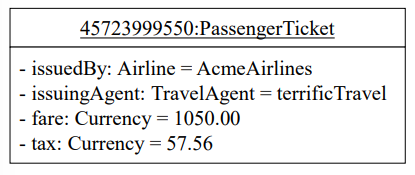
\includegraphics[width=0.5\textwidth]{assets/uml_instanceof1.png}} \hfill
		\subfloat[]{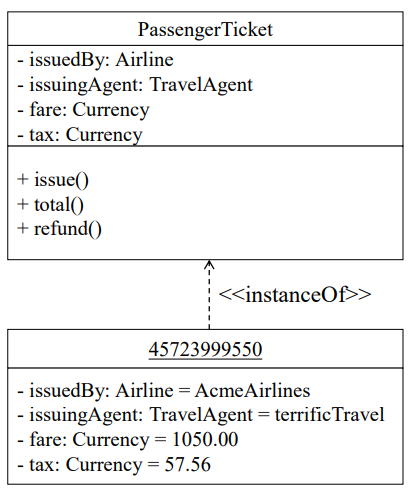
\includegraphics[width=0.5\textwidth]{assets/uml_instanceof2.png}}
		\label{fig:subfig}
	\end{figure}

	\subsection{Ereditarietà}
	Nella progettazione e programmazione OO una relazione fondamentale, e caratteristica fondamentale del paradigma object-oriented, è quella esistente fra le classi: la \textbf{relazione di ereditarietà} (inheritance).
	\vspace{\baselineskip} \\
	Una classe è considerata come un \textit{repertorio di conoscenze} a partire dal quale è possibile definire altre \textit{classi più specifiche}, che completano le conoscenze della loro classe madre.
	\vspace{\baselineskip} \\
	Una \textbf{sottoclasse}, è dunque una \textit{specializzazione} della descizione di una classe, detta la sua \textbf{superclasse}, della quale essa mutua (parte di) gli attributi e i metodi. Concettualmente è come se le informazioni della superclasse fossero ricopiate nella sottoclasse. A livello fisico, comunque, le duplicazioni sono evitate.
	\vspace{\baselineskip} \\
	Ci sono diverse forme di ereditarietà.

	\subsubsection{Ereditarietà per estensione (extension inheritance)}
	La forma più comune di ereditarietà è quella per estensione. In questo caso, una sottoclasse estende la superclasse aggiungendo nuovi attributi e/o nuovi metodi non presenti nella superclasse e non applicabili a istanze della superclasse.
	\vspace{\baselineskip} \\
	La visibilità (pubblica, protetta, privata, package) degli attributi e delle operazioni ereditate dalla superclasse non è modificata.
	\begin{center}
		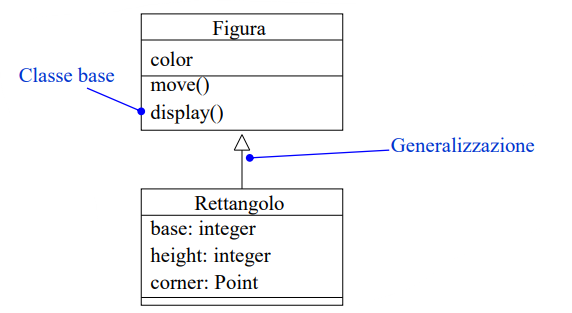
\includegraphics[scale=0.7]{assets/ereditarieta_estensione.png}
	\end{center}
	La superclasse non conosce le classi figlie. Le classi figlie conoscono la superclasse.

	\subsubsection{Ereditarietà per variazione funzionale (functional variation inheritance)}
	In questo caso, si ridefiniscono alcune caratteristiche (metodi) della superclasse quando quelle ereditate si rivelano inadeguate per l'insieme di oggetti descritti dalla sottoclasse.
	\vspace{\baselineskip} \\
	La ridefinizione (\textbf{override}) del metodo ereditato riguarda solo l'implementazione e non la segnatura (nome, parametri formali e parametri di ritorno).
	\vspace{\baselineskip} \\
	Ogni richiesta di esecuzione del metodo ridefinito da parte di un oggetto della sottoclasse farà riferimento alla nuova implementazione fornita nella sottoclasse.
	\paragraph*{Esempio} Nella classe \textit{ContoCorrente} il metodo \textit{preleva} controlla che il conto non vada in rosso. Il metodo \textit{preleva} della classe \textit{ContoCorrenteConFido} ridefinisce il metodo della superclasse per controllare che il prelievo non vada oltre il fido concesso. \\
	Se cambiano le regole del contesto occorre modificare il metodo preleva di \textit{ContoCorrente}, ma la modifica non viene riportata automaticamente anche all classe \textit{ContoCorrenteConFido}.
	\begin{center}
		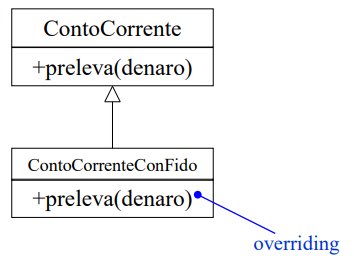
\includegraphics[scale=0.7]{assets/ereditarieta_variazione_funzionale.png}
	\end{center}
	La ridefinizione non è incrementale, quindi i cambiamenti nel metodo originale devono essere riportati anche nei metodi ridefiniti. Purtroppo non c'è alcuna garanzia che questo accada e si possono introdurre degli errori.
	\vspace{\baselineskip} \\
	Anche nell'ereditarietà per variazione funzionale, la visibilità (pubblica, protetta, privata, package) degli attributi e delle operazioni ereditate dalla superclasse non è modificata. \\
	Osserviamo inoltre che la variazione funzionale attiene solo le operazioni di accesso e trasformazioni di una classe e non i costruttori degli oggetti.

	\subsubsection{Principio di sostituibilità}
	Data una dichiarazione di una variabile o di un parametro il cui tipo è dichiarato come X, una qualunque istanza di una classe che è discendente di X può essere usato come valore effettivo senza violare la semantica della dichiarazione e il suo uso.
	\\
	In altri termini, l'istanza di una sottoclasse può essere usata al posto di un'istanza della superclasse senza che il comportamento del programma cambi.
	\vspace{\baselineskip} \\
	Il principio di sostituibilità è alla base del polimorfismo di inclusione, nella programmazione orientata a oggetti. Questo principio è stato introdotto dalla Prof.ssa Barbara Liskov del MIT nel 1987.
	\vspace{\baselineskip} \\
	Di conseguenza, una sottoclasse non può rimuovere o rinunciare a proprietà/metodi della superclasse. Altrimenti una istanza della sottoclasse non sarà sostituibile in una situazione in cui si dichiara l'uso di istane della superclasse.
	\vspace{\baselineskip} \\
	In effetti, preservando la visibilità degli attributi e dei metodi ereditati, così come accade nelle precedenti forme di ereditarietà viste, si garantisce che gli oggetti della sottoclasse offrano quanto meno gli stessi servizi degli oggetti della superclasse (anche se i servizi potranno essere implementati diversamente).
	\vspace{\baselineskip} \\
	Pertanto il principio di sostituibilità (o polimorfismo di inclusione) è compatibile con l'ereditarietà per estensione e variazione funzionale.

	\subsubsection{Ereditarietà e relazione is\_a}
	Nell'ereditarietà per estensione e per variazione funzionale, la relazione di ereditarietà fra classi corrisponde a una relazione di \textbf{generalizzazione} (o \textbf{is\_a}). Ciò perchè ogni istanza di una classe derivata da una classe base va considerata come (è anche) una istanza della classe base.
	Il simbolo $\uparrow$ usato in UML denota un generalizzazione.
	\paragraph*{Esempio} Le istanze di Rettangolo cono anche istanze di Figura.

	\subsubsection{Ereditarietà di implementazione (implementation inheritance)}
	In questo caso, una sottoclasse utilizza il codice della superclasse (definizioni di attributi e metodi) per implementare l'astrazione associata.
	\paragraph*{Esempio} Una classe \textit{Vettore} mette a disposizione una rappresentazione di un vettore, un costruttore, un metodo di accesso (ad un elemento sulla base dell'indice) e uno di trasformazione (cambiamento di stato di un elemento di cui si conosce la posizione).
	\vspace{\baselineskip} \\
	Una classe \textit{Pila} può essere definita come sottoclasse di \textit{Vettore}, in modo da potersi basare sulla rappresentazione del vettore per poter rappresentare una pila. Si dice che la realizzazione del dato astratto \textit{Pila} è delegata a quella del vettore. Se si cambia la rappresentazione del vettore si cambia anche quella della pila.
	\vspace{\baselineskip} \\
	Grazie all'ereditarietà per implementazione, la realizzazione degli operatori \textit{push, pop, top} previsti per una pila può basarsi sugli operatori messi a disposizione dalla classe \textit{Vettore}. \\
	Si noti bene che la \textit{Pila} ha un diverso insieme di operatori rispetto a quelli del \textit{Vettore}. L'ereditarietà riguarda solo la realizzazione del vettore e l'implementazione dei metodi, non l'interfaccia della classe (ciò che è visibile agli utilizzatori di \textit{Vettore}).
	\vspace{\baselineskip} \\
	Pertanto l'ereditarietà di implementazione comporta la modifica alla visibilità delle caratteristiche ereditate.
	\vspace{\baselineskip} \\
	L'ereditarietà a base privata supportata dal C++ e da Ada-95 permette di rendere privati gli attributi e gli operatori pubblici ereditati. \\
	Visibilità con ereditarietà a base pubblica:
	\begin{center}
		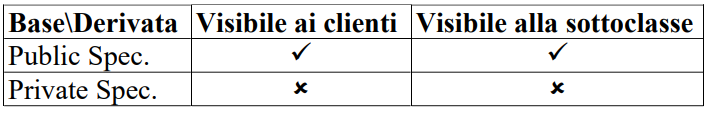
\includegraphics[scale=0.7]{assets/ereditarieta_base_pubblica.png}
	\end{center}
	Visibilità con ereditarietà a base privata:
	\begin{center}
		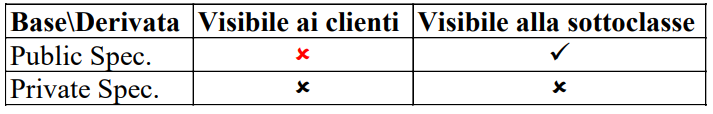
\includegraphics[scale=0.7]{assets/ereditarieta_base_privata.png}
	\end{center}
	In UML l'ereditarietà di implementazione è indicata utilizzando lo stesso simbolo della generalizzazione, ma specificando a fianco lo stereotipo $<<$implementation$>>$.
	\begin{center}
		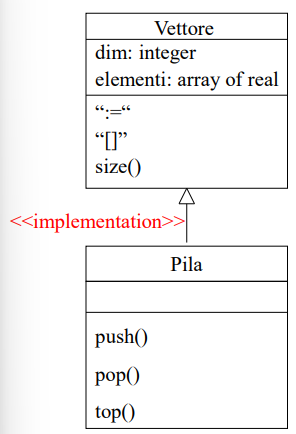
\includegraphics[scale=0.7]{assets/ereditarieta_impl.png}
	\end{center}
	L'ereditarietà di implementazione non è compatibile con il principio di sostituibilità. Pertanto se la classe Y eredita solo l'implementazione della classe X, non si può riutilizzare su istanze di Y tutto il codice in cui si dichiarano e utilizzano dati di classe X, in quanto non vale il polimorfismo di inclusione.
	\vspace{\baselineskip} \\
	L'ereditarietà di implementazione permette un riuso \textbf{parziale} del codice.

	\subsubsection{Combinazione di ereditarietà}
	Nella progettazione di una classe si possono combinare diverse forme di ereditarietà.
	\paragraph*{Esempio} La classe \textit{ContoCorrenteConFido} implementa l'ereditarietà per estensione, aggiungendo il metodo \textit{impostaFido} e per variazione funzionale ridefinendo il metodo \textit{preleva}.
	\begin{center}
		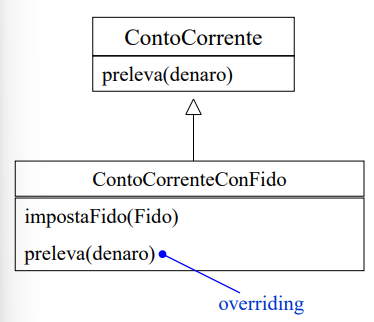
\includegraphics[scale=0.7]{assets/ereditarieta_combinazione.png}
	\end{center}

	\subsubsection{Proprietà della relazione di ereditarietà}
	La rappresentazione della relazione di generalizzazione fra un insieme di classi definisce un \textbf{grado di ereditarietà} che è un \textbf{grafo orientato aciclico}. La relazione di generalizzazione è transitiva e antisimmetrica:
	\begin{itemize}
		\item la transitività comporta che le caratteristiche delle classi superiori sono ereditate dalle classi inferiori.
		\item l'antisimmetria definisce una direzione di attraversamento del grafo di ereditarietà che porta dalla sottoclasse alla superclasse.
	\end{itemize}
	Partendo da una classe C e seguendo la direzione che porta al genitore, si trovano tutte le classi \textbf{antenate}, che per estensioni sono chiamate \textbf{superclassi} di C. Seguendo la direzione opposta di trovano tutte le classi \textbf{discendenti} di C.
	\begin{center}
		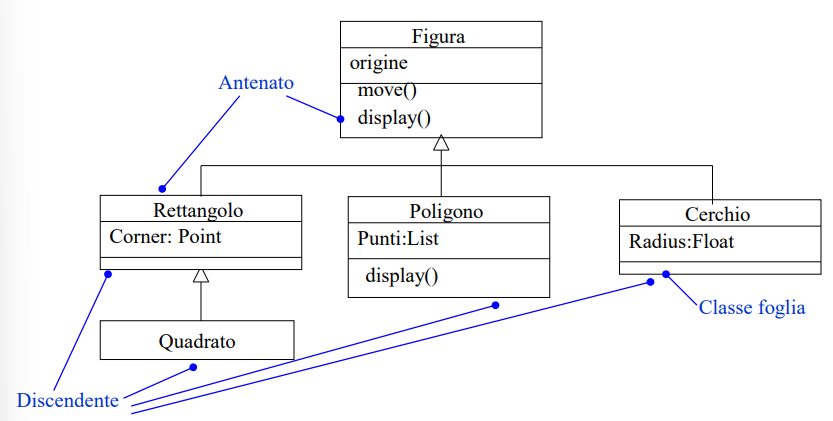
\includegraphics[scale=0.5]{assets/ereditarieta_grafo.png}
	\end{center}
	Ogni classe C ha il proprio \textbf{grafo di ereditarietà G(C)} che è una restrizione del grafo di ereditarietà completo delle sole superclassi della classe in esame.

	\subsubsection{Ereditarietà singola}
	In questo caso specifico, il grafo è in realtà un albero: ogni classe ha una sola superclasse diretta. Si dice che l'ereditarietà è \textbf{semplice} o \textbf{singola}.
	\vspace{\baselineskip} \\
	Il grafo di ereditarietà G(C) di una classe C è una catena di antenati. Gli elementi della catena sono ordinati secondo una relazione d'ordine totale. Poichè un metodo può essere ridefinito in più classi si pone il seguente
	\paragraph*{Problema} Sia dato un metodo m, eventualmente ereditato, della classe $C_1$. Da quale classe $C_2 in G(C_1)$ si eredita m?
	\paragraph*{Soluzione}
	\begin{enumerate}
		\item Passo: si determina catena di antenati di $C_1$
		\item Passo: si ricerca la prima occorrenza della (ri-)definizione di m a partire dall'estremità $C_1$ della catena.
	\end{enumerate}

	\subsubsection{Ereditarietà multipla}
	Una classe può avere più superclassi. In questo caso si parla di ereditarietà \textbf{multipla}.
	\paragraph*{Esempio}: La classe \textit{Orologio} necessita dei servizi messi a disposizione sia da \textit{Data} che da \textit{Tempo}. In più ne implementa degli altri.
	\vspace{\baselineskip} \\
	Il grafo di ereditarietà non è più un albero. Data una classe C, G(C) non è più una catena ma un grafo aciclico orientato. L'ordine fra le classi in G(C) è parziale.
	\begin{center}
		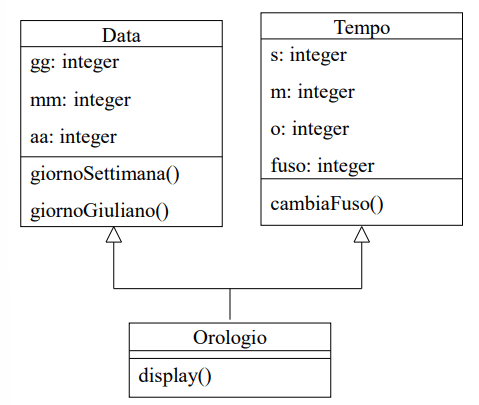
\includegraphics[scale=0.5]{assets/ereditarieta_multipla.png}
	\end{center}
	Anche nell'ereditarietà multipla un metodo può essere ridefinito in diverse classi e si pone il seguente
	\paragraph*{Problema}: Sia dato un metodo m, eventualmente ereditato, della classe $C_1$. Da quale classe $C_2 in G(C_1)$ si eredita m?
	\begin{center}
		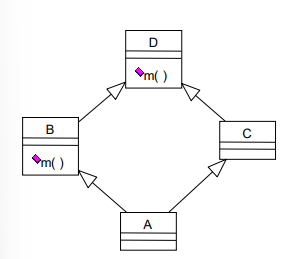
\includegraphics[scale=0.7]{assets/ereditarieta_multipla_problema.png}
	\end{center}
	Se $C_1$=A c'è un conflitto fra le diverse definizioni di m in B e D, entrambe ereditabili. Il conflitto può essere risolto in questo caso. Si considera una qualunque \textit{linearizzazione} del grafo G($C_1$). i possono avere due casi:
	\begin{itemize}
		\item $A \rightarrow B \rightarrow C \rightarrow D$
		\item $A \rightarrow C \rightarrow B \rightarrow D$
	\end{itemize}
	In entrambi i casi, B precede D, il che significa che il metodo m è ereditato da B. Il metodo m di B è quello più specifico e maschera quello omonimo di D. \\
	Le due linearizzazioni del grafo $G(C_1)$, precedentemente specificate, non aiutano a scegliere.
	\vspace{\baselineskip} \\
	Esistono dei criteri euristici per gestire queste situazioni conflittuali:
	\begin{enumerate}
		\item \textbf{molteplicità dell'ereditarietà}: nel definire che A deriva dalle due superclassi occorrerà elencarle in un qualche ordine:
		\begin{center}
			$A \rightarrow B,C$ piuttosto che $A \rightarrow C,B$
		\end{center}
		L'ordine delle classi è utilizzato per preferire una delle due linearizzazioni. Tuttavia questo principio può essere in contraddizione con quello che indica di preferire l'ereditarietà da classi più specifiche. Esempio:
		\begin{center}
			$A \rightarrow B,C$ e $C \rightarrow B,D$
		\end{center}
		Se m è definito in B e in C si dovrebbe preferire C in quanto C precede sempre B nelle linearizzazioni:
		\begin{center}
			$A \rightarrow C \rightarrow B \rightarrow D$
		\end{center}
		\item \textbf{modularità}: si può scomporre un grafo di ereditarietà in moduli che corrispondono ai diversi punti di vista sull'oggetto. \\
		Per esempio, i diversi moduli corrispondono ai diversi punti di vista (tipo alimentazione, tipo articolo, casa costruttrice).
		\begin{center}
			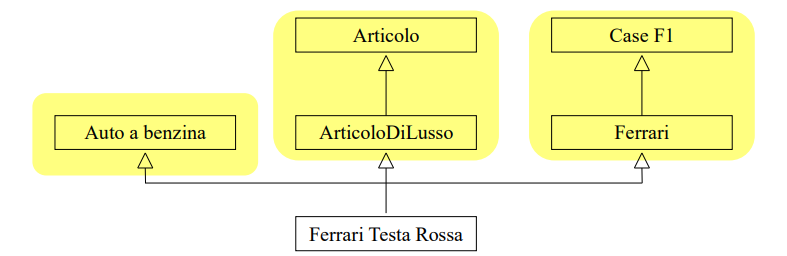
\includegraphics[scale=0.5]{assets/ereditarieta_multipla_modularita.png}
		\end{center}
		Nelle linearizzazioni non ci sono relazioni di ereditarietà tra classi appartenenti a moduli diversi. Anche in queto caso potrebbero esserci contraddizioni da risolvere specificando l'ordinamento dei moduli.
	\end{enumerate}
	Quste contraddizioni mettono in evidenza le difficoltà che si incontrano a dare una semantica a un metodo quando si permette l'ereditarietà multipla.\\
	I diversi principi per gestire le situazioni conflittuali non sono universalmente accettati. La risoluzione dei conflitti, in realtà, non può essere efficace se non prende in considerazione le conoscenze specifiche legate all'applicazione. \\
	Per questo molti sconsigliano l'ereditarietà multipla, in qunato i benefici sono pochi mentre i problemi legati ad una semantica ben definita sono molti.

	\subsubsection{Visibilità protetta}
	La relazione di ereditarietà introduce un ulteriore livello di visibilità, la \textbf{visibilità protetta (protected)}. Un attributo o un metodo con visibilità protetta è visibile solamente all'interno della classe stessa, delle classi del package e delle classi discendenti (anche in altri package).

	\subsection{Classi astratte}
	Se in programmazione object-oriented non può esistere un oggetto senza che sia stata creata la classe di appartenenza (come invece accade in ADA), è invece possibile che esistano classi per le quali non è possibile generare delle istanze (\textbf{classi astratte}). \\
	Una classe astratta può essere una classe non completamente specificata. In particolare, non è definito il metodo corrispondente ad una operazione (i metodo è astratto). \\
	Una classe astratta è una classe che non può essere istanziata perchè il comportamento dei suoi oggetti non sarebbe completamente definito (ha senso come superclasse di una classe concreta istanziabile). \\
	La realizzazione di ereditarietà riguarda anche le classi astratte.

	\subsubsection{Notazione}
	Una classe o un metodo astratto è indicato con il nome in italico. Nel metodo astratto viene eridata solo la segnatura e non ha nè semantica nè implementazione. Per esempio:
	\begin{center}
		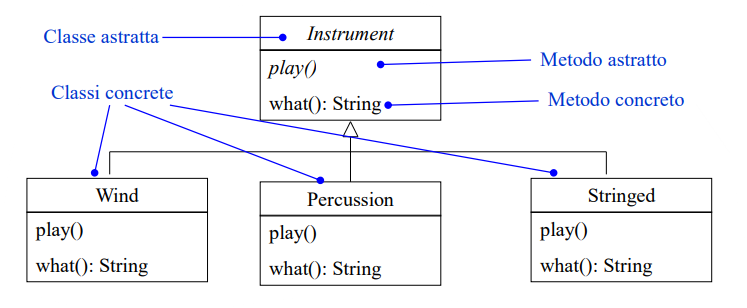
\includegraphics[scale=0.5]{assets/classi_astratte_notazione.png}
	\end{center}
	La classe strumenti musicali è astratta perchè non possiamo definire il metodo \textit{play}. Esso è imolementato nelle sottoclassi degli strumenti a fiato, a percussione e nei cordati. Il metodo what è invece concreto (è implementato) e restituisce il nome della classe. Esso è ridefinito in ogni classe.
	\vspace{\baselineskip} \\
	Le classi astratte sono strumenti per fattorizzare proprietà comuni tra classi simili e poterle organizzare in una gerarchia di ereditarietà. Non potremo mai creare oggetti a partire da una classe astratta, ma possiamo servircene per dare una radice comune a un insieme di classi che condividono le stesse proprietà e poter quindi sfruttare il polimorfismo di inclusione e il binding dinamico (di cui si parlerà in seguito). \\
	Le classi astratte fungono da \textbf{serbatoi di ereditarietà}.
	\paragraph*{Esempio:}
	\begin{center}
		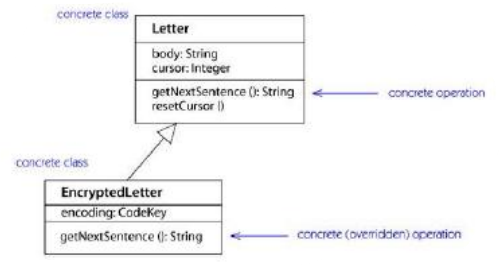
\includegraphics[scale=0.7]{assets/classi_astratte_esempio.png}
	\end{center}
	La classe Letter ha un metodo che restituisce la frase successiva da leggere e l'operazione resetCursor che riporta all'inizio del testo. La sottoclasse EncriptedLetter rappresenta una lettera crittografata. Il metodo getNextSentence è stato sovrascritto perché il testo dev'essere decrittato prima di essere restituito. L'implementazione dell'operazione getNextSentence è completamente diversa da quella ereditata. PROBLEMA: Il progettista di EncriptedLetter non ha alcuna informazione per comprendere quale metodo di Letter dev'essere sovrascritto.
	\begin{center}
		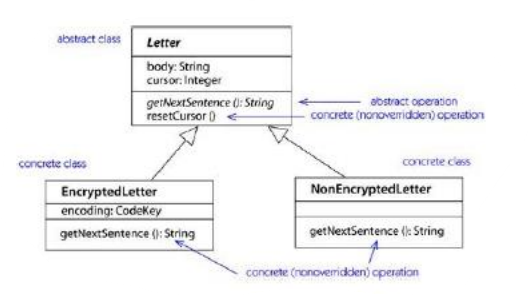
\includegraphics[scale=0.7]{assets/classi_astratte_esempio_update.png}
	\end{center}
	Se il metodo \textit{getNextSentence} di Letter fosse astratto (e dunque fosse astratta anche la classe \textit{Letter}) il progettista verrebbe informato della necessità di ridefinire il metodo. La classe astratta \textit{Letter} fattorizza i metodi concreti comuni alle sue sottoclassi, come resetCursor.

	\subsection{Classi Finali}
	Una classe è detta \textbf{finale (final)} o foglia (leaf) quando non può essere ulteriormente specializzata, e quindi non può essere modificata. \\
	Si definisce una classe foglia quando il comportamento della classe dev'essere ben stabilito per ragioni di \textbf{affidabilità}. \\
	La dichiarazione di una classe foglia permette anche la generazione di codice ottimizzato in quanto facilita l'espansione in linea del codice (impossibile nel caso di metodi sovrascrivibili nelle sottoclassi). \\
	Non ha senso stabilire una classe astratta foglia. 

	\subsection{Class Diagram in dettaglio}
	\begin{center}
		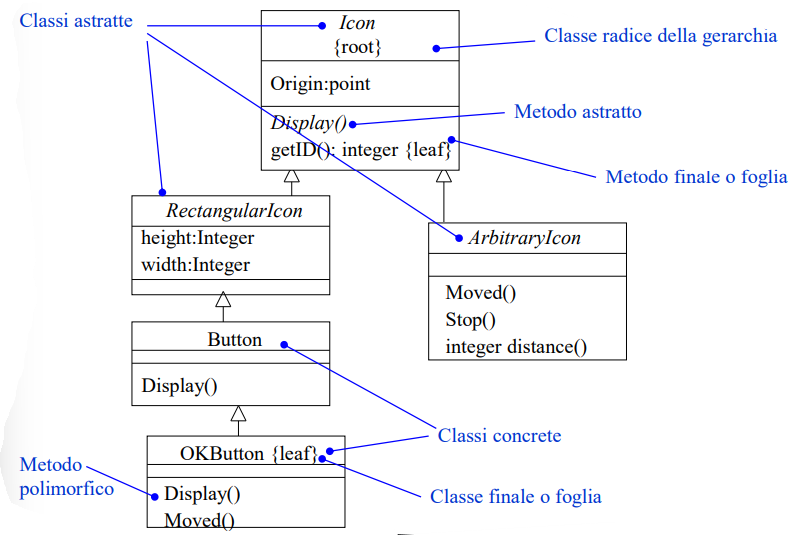
\includegraphics[scale=0.5]{assets/class_diagram.png}
	\end{center}
	Un metodo concreto leaf non può avere override, mentre un metodo astratto leaf da errore. \\
	Mettere leaf i metodi di una classe leaf è inutile ma non sbagliato. \\
	La classe astratta \textit{ArbitraryIcon} non ha senso poichè non ha discendenti, ma non è sbagliata.

	\subsection{Interfacce}
	Una interfaccia è la descrizione del comportamento degli oggetti senza specificarne una implementazione. Essa è una collezione di operazioni, cioè di servizi che possono essere richiesti, priva di informazioni sulle implementazioni dei servizi (i metodi).
	\vspace{\baselineskip} \\
	Similmente ad una classe, un'interfaccia può avere un qualsiasi numero di operazioni. Diversamente invece, un'interfaccia non specifica la struttura (non sono inclusi attributi, se non statici) e non fornisce un'implementazione (non sono specificati i metodi che implementano le operazioni). Di conseguenza le interfacce non possono essere istanziate.
	\vspace{\baselineskip} \\
	Una interfaccia è simile ad una classe astratta i cui metodi son tutti astratti e non dispone di attributi.
	\vspace{\baselineskip} \\
	Nella sua rappresentazione più generale, un'interfaccia è rappresentata mediante l'utilizzo di un cerchio, sopprimendo la visualizzazione delle operazioni. Tuttavia, se lo si ritiene importante per la comprensione del modello, è possibile modellare un'interfaccia come una classe stereotipata
	\begin{center}
		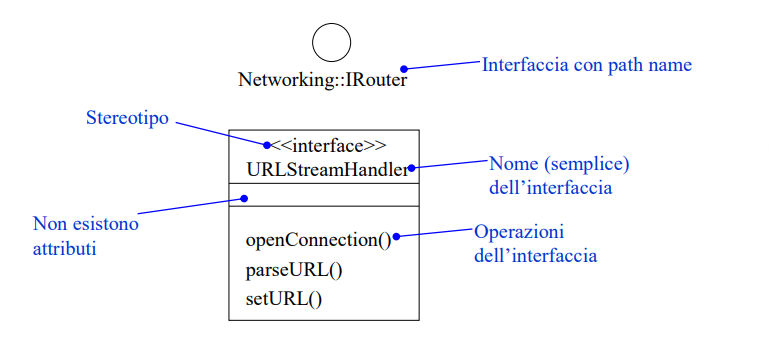
\includegraphics[scale=0.5]{assets/interfacce.png}
	\end{center}
	Una o più classi possono realizzare/implementare le operazioni indicate in una interfaccia. La relazione che si stabilisce fra una interfaccia e una classe che la implementa è detta relazione di realizzazione. In UML è indicata con una freccia tratteggiata.
	\begin{center}
		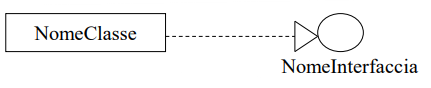
\includegraphics[scale=0.5]{assets/relazione_realizzazione_esempio.png}
	\end{center}
	La relazione di realizzazione si presenta come un valido strumento per scindere la specifica di un "contratto" (cosa una classe deve implementare) e la sua implementazione (come si rendono i servizi del contratto).
	\paragraph*{Esempio} l'interfaccia \textit{java.lang.Comparable} specifica una sola operazione.
	\begin{center}
		\textit{public int compareTo(Object o)}
	\end{center}
	che prende un oggetto generico \textit{Object} come argomento e restituisce un valore negativo se l'argomento è più piccolo dell'oggetto corrente, zero se è uguale e un valore positivo se è maggiore. \\
	Una qualunque classe che implementa questa interfaccia deve fornire una implementazione (un metodo) per \textit{compareTo}.
	\vspace{\baselineskip} \\
	Le interfacce servono a disaccoppiare la definizione delle operazioni dalla loro implementazione. Per poter usare un certo oggetto è sufficiente conoscere la sua interfaccia: non serve conoscere l'implementazione.
	\paragraph*{Esempio} Il metodo sort della classe Arrays, che ordina un array di oggetti utilizzando l'algoritmo di ordinamento per fusioni successive (mergesort), necessita solo di sapere che gli elementi dell'array offrono il servizio compareTo, in modo da poterli confrontare. Non serve sapere "come" si realizza il servizio, cioè come sono effettivamente confrontati gli oggetti. Si crea così una dipendenza di implementazione fra la classe Arrays e l'interfaccia Comparable.
	\begin{center}
		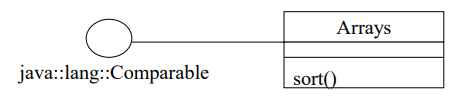
\includegraphics[scale=0.5]{assets/relazione_realizzazione_esempio2.png}
	\end{center}
	UML permette di rappresentare in modo compatto le seguenti relazioni:
	\begin{center}
		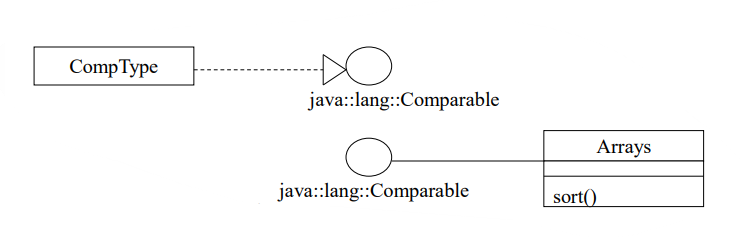
\includegraphics[scale=0.5]{assets/relazione_realizzazione_esempio3.png}
	\end{center}
	attraverso la notazione:
	\begin{center}
		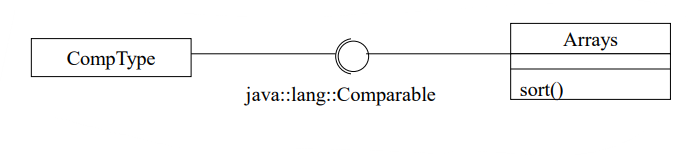
\includegraphics[scale=0.5]{assets/relazione_realizzazione_esempio4.png}
	\end{center}
	Anche le interfacce possono ereditare da altre interfacce. Poichè non ci sono implementazioni, la realizzazione di ereditarietà è naturalmente una relazione di generalizzazione "is\_a". 
	\vspace{\baselineskip} \\
	Le interfacce sono realizzabili in java e non presentano il problema dell'ereditarietà multipla con le operazioni comuni nelle superclassi. E' valida solo l'ereditarietà per estensione. \\
	Poichè non si considerano le implementazioni delle operazioni, l'ereditarieta' multipla su interfacce non pone problemi di conflitto di realizzazione.\\ 
	Per questo alcuni linguaggi di programmazione, come Java, permettono  l'ereditarietà singola sulle classi (in quanto specificano anche le implementazioni) mentre permettono l'ereditarietà multipla sulle interfacce. \\
	Questo distingue le classi astratte (per le quali l'ereditarietà multipla può porre dei problemi riguardo ai metodi implementati) dalle interfacce. Ad esempio:
	\begin{center}
		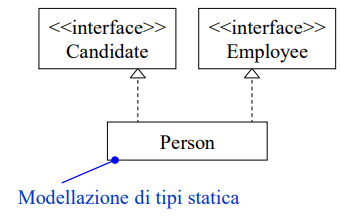
\includegraphics[scale=0.5]{assets/realizzazione_piu_interfacce.png}
	\end{center}
	Poiché non possono sorgere problemi di conflitto di realizzazione, è permesso a una classe di realizzare più interfacce, per di più non correlate da una relazione di generalizzazione. 	In questo modo tutto il codice scritto per Candidate e Employee può essere utilizzato su oggetti di classe Person. \\	\\
	Infine, più classi possono implementare la stessa interfaccia. E' questo il caso di una interfaccia definita per dati astratti molto utilizzati nello sviluppo del software, come pile, code, liste, alberi e grafi, per le quali sono possibili molteplici realizzazioni che variano per l'efficienza degli operatori. Ad esempio:
	\begin{center}
		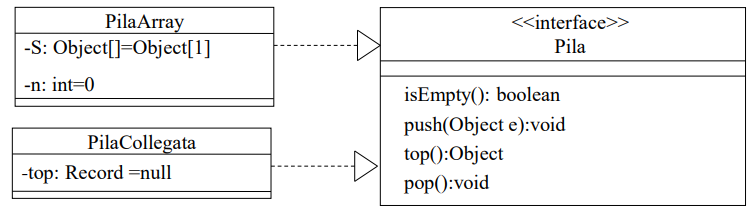
\includegraphics[scale=0.5]{assets/realizzazione_multiple_interfaccia.png}
	\end{center}
	Il codice applicativo che intende fare uso di una pila dichiarerà delle variabili di tipo Pila, svincolandosi dalla specifica realizzazione. Questa sarà specificata solo al momento della inizializzazione della variabile. Si garantisce così una forte invarianza ai cambiamenti delle realizzazioni di una pila.

	\subsection{Aggregazione di oggetti}
	L'ereditarietà offre molti vantaggi, ma non tutti gli oggetti si ottengono bene \textbf{derivandoli} da altri oggetti. Spesso un oggetto è ottenuto \textbf{aggregando} altri oggetti.
	\paragraph*{Esempio}
	Ricorrendo all'ereditarietà multipla è allettante definire una classe Automobile partendo dalle classi Carrozzeria, Sedile, Ruota e Motore. Si tratta di un errore concettuale poiché l'ereditarietà multipla permette di definire due oggetti per fusione e non per composizione. Un'automobile è composta da una carrozzeria, da un motore, da sedili e da ruote; ma il suo comportamento non è in alcun caso l'unione dei comportamenti di queste differenti parti.
	\vspace{\baselineskip} \\
	Nell'esempio specifico, sembrerebbe che il ricorso all'ereditarietà di implementazione sia la soluzione. Essa permette il riuso della sola implementazione (attributi e metodi) ma non dei comportamenti. \\
	Ma neanche questa forma di ereditarietà è adatta allo scopo. Infatti, ereditando dalla classe Ruota si ha la possibilità di rappresentare e manipolare una sola ruota, mentre un'automobile ha quattro ruote.
	\vspace{\baselineskip} \\
	Una \textbf{composizione di oggetti} può essere rappresentata permettendo alle variabili di istanza di una classe di puntare a oggetti di altre classi. Si possono stabilire legami con più istanze di una classe che descrive un componente. La relazione che si stabilisce in questo modo fra le classi è detta di \textbf{aggregazione} o \textbf{composizione} (o relazione "has\_a"). Essa è quindi un'altra possibile relazione fra le classi, diversa dall'ereditarietà e dalla generalizzazione (o "is\_a"). Una classe A si dice in relazione di aggregazione con una classe B quando alcune istanze di B contribuiscono a formare una parte delle isstanze di A. L'aggregazione è, come l'ereditarietà, una relazione asimmetrica.
	\vspace{\baselineskip} \\
	In UML, l'aggregazione è resa mediante una linea piena e un piccolo rombo dalla parte del contenitore. L'aggregazione vale solo tra classi, non tra interfacce. La molteplicità consente di indicare quanti oggetti possono essere aggregati.
	\paragraph*{Esempio}
	\begin{center}
		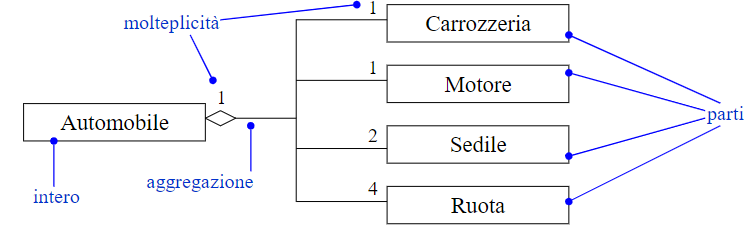
\includegraphics[scale=0.5]{assets/aggregazione_notazione.png}
	\end{center}
	L'suo dell'aggregazione è consigliato nelle seguenti stituazioni:
	\begin{itemize}
		\item Contenimento fisico: la pagina di un libro
		\item Appartenenza: il giocatore di una squadra di calcio
		\item Composizione funzionale: le ruote di una automobile
	\end{itemize}
	Si deve osservare che \textbf{l'aggregazione non implica una dipendenza esistenziale}: un'automobile può essere distrutta ma alcune sue parti possono essere riutilizzate. Una squadra di calcio può fallire, ma i suoi giocatori non vengono "soppressi".

	\subsection{Composizione di oggetti}
	Le aggregazioni sono associazioni \textbf{deboli} fra parti e intero. Questo significa che le parti possono esistere senza l'intero.
	\vspace{\baselineskip} \\
	Un'associazione \textbf{forte} fra parti e intero è detta \textbf{composizione} e si rappresenta in UML mediante un rombo pieno. La composizione comporta una \textbf{dipendenza esistenziale}, in quanto le parti non esistono senza il contenitore. \\
	Ciò presuppone che la crezione e la distruzione delle parti avvengano nel contenitore e che i componenti non siano parti di altri oggetti.
	\paragraph*{Esempi}
	In questi esempi, la vita delle parti che compongono l'intero dipende dalla vita dell'intero stesso:
	\begin{enumerate}
		\item i dipartimenti non esisterebbero se non esistesse la società;
		\item il tempo di vita dei diversi oggetti grafici di interazione dipende da quello della finestra che li contiene.
	\end{enumerate}
	\paragraph*{Esempio}
	\begin{center}
		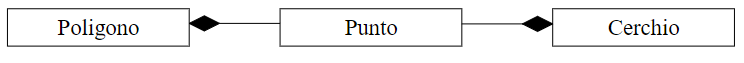
\includegraphics[scale=0.5]{assets/composizione_punto.png}
	\end{center}
	Un'istanza di Punto può essere parte di un poligono oppure il centro di un cerchio, ma non entrambe le cose.
	\paragraph*{Regola di non condivisione}
	Benchè una classe possa essere componente di molte altre classi, \textbf{ogni sua istanza può essere componente di un solo oggetto}. Un diagramma delle classi può mostrare più classi di potenziali possessori di oggetti componenti, ma ogni istanza di componente deve appartenere ad un solo oggetto possessore. Questa regola è caratterizzante della composizione.
	\vspace{\baselineskip} \\
	La composizione fra classi stabilita in fase di progettazione offre delle informazioni importanti al programmatore che andrà a implementare le classi.\\
	Ad esempio, se il programmatore utilizzerà il C++ farà si che gli oggetti componenti finiscano nello stack e non nello heap (non userà puntatori/new).\\
	Se utilizza il Java, che pone tutto nello heap, si preoccuperà di allocare i componenti nella classe contenitore e di non passare mai all'esterno della classe il riferimento ai componenti, in modo da impedirne la condivisione con oggetti di altre classi (il componente sarà privato e non ci sarà alcun metodo che restituisce il suo riferimento).
	
	\subsection{Ereditarietà vs aggregazione}
	In molti casi è possibile associare due classi mediante ereditarietà o aggregazione/composizione e la scelta non è immediata come negli esempi visti precedentemente. \\
	Per esempio si supponga di disporre di una classe Data e di una classe Tempo, che rappresentano e manipolano, rispettivamente, date e istanti di tempo. Volendo definire una nuova classe Orologio per rappresentare sia le date che gli istanti di tempo, si può:
	\begin{enumerate}
		\item derivare Orologio da Data e da Tempo, se l'ereditarietà multipla è permessa;
		\item comporre Orologio con le due classi.
	\end{enumerate}
	Sono anche possibili soluzioni ibride, come derivare Orologio da Data e comporlo con Tempo.
	Le differenze tra la scelta 1) e la 2) sono:
	\begin{itemize}
		\item Nell'ereditarietà, ogni oggetto \textit{o} della classe \textit{Orologio} contiene tutti i campi definiti nelle classi \textit{Data} e \textit{Tempo} e può accedervi direttamente se non sono privati.
		\item Nell'aggregazione/composizione, ogni oggetto \textit{o} della classe \textit{Orologio} contiene due campi di tipo \textit{Data} e \textit{Tempo} rispettivamente. Per accedere all'informazione sul giorno occorrerà invocare un metodo (per esempio \textit{day()}) sull'oggetto \textit{D}.
		\item Se l'\textbf{ereditarietà} corrisponde a una relazione di generalizzazione "is\_a" \textbf{vale il polimorfismo di inclusione}, cioè ogni oggetto di \textit{Orologio} è utilizzabile come istanza di \textit{Data} e di \textit{Tempo}, \textbf{mentre questo non è vero nel caso della composizione}.
	\end{itemize}
	Le scelte di progetto sono totalmente diverse.
	\begin{itemize}
		\item L'ereditarietà permette di poter "dimenticare" il fatto che \textit{gg} è definito nella classe \textit{Data} e di utilizzarlo direttamente come campo di \textit{Orologio} (sempre che sia definito come \textit{protected} e non come \textit{private}). Questa caratteristica della derivazione è particolarmente utile se si vogliono utilizzare più derivazioni successive e creare vere e proprie gerarchie di classi. In questo caso non è necessario conoscere a quale livello della gerarchia è definito un dato campo, ma è possibile utilizzarlo direttamente come se fosse un elemento della classe stessa.
		\item L'ereditarietà permette di riutilizzare tutti i metodi delle varie classi che operano su oggetti delle classi \textit{Data} e \textit{Tempo}.
	\end{itemize}
	\paragraph*{Esempio}
	\textit{Agenda} ha due metodi che possono operare anche su istanze di \textit{Orologio}. Il codice dei metodi polimorfi \textit{move} è riutilizzabile per istanze di \textit{Orologio}.
	\begin{center}
		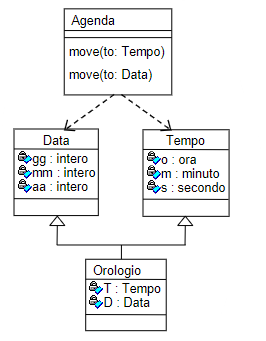
\includegraphics[scale=0.5]{assets/ereditarieta_vs_aggregazione.png}
	\end{center}
	\textbf{Il meccanismo di aggregazione/composizione} è generalmente usato quando si vogliono utilizzare i servizi di una classe predefinita ma \textbf{non la sua interfaccia}. L'ereditarietà di implementazione, qualora non dovesse essere permessa da un linguaggio di programmazione, potrebbe essere resa da una relazione di aggregazione/composizione.

	\subsection{Raggruppare classi}
	La mole di classi aumenta in modo considerevole all'aumentare della complessità del sistema da modellare. E' importante organizzare tali classi in \textbf{gruppi} separati al fine di rendere più facilmente individuabili e accessivili le singole parti che compongono il nostro sistema. \\		
	I \textbf{package} sono un meccanismo generale per organizzare le classi in gruppi. \\
	In UML un package è rappresentato come segue:
	\begin{center}
		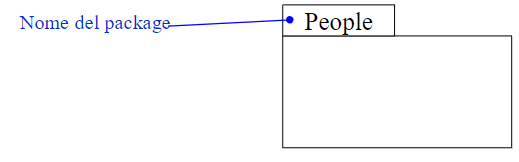
\includegraphics[scale=0.5]{assets/package_uml.png}
	\end{center}
	In genere i package si usano per riunire classi, ma nella notazione UML essi possono includere qualsiasi costrutto UML e possono essere persino eterogenei. \\
	E' consenrtito mostrare il contenuto di un package sia testualmente sia graficamente:
	\begin{center}
		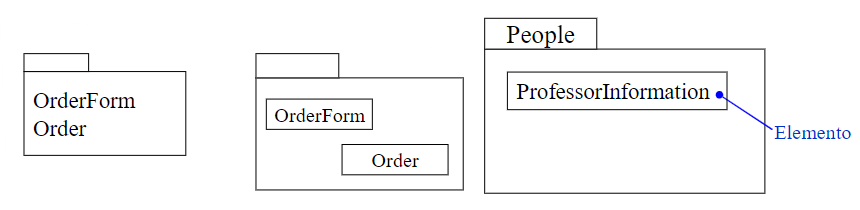
\includegraphics[scale=0.5]{assets/package_uml_contenuto.png}
	\end{center}
	Un package definisce un \textbf{namespace} (spazio degli identificatori) per i suoi elementi. Questo significa che ogni classe di un package di classi deve avere un nome distinto all'interno del package che la racchiude. Il nome completo (o \textbf{qualificato}) della classe sarà ottenuto indicato tramite la notazione nomepackage::nomeclasse. \\
	In generale é possibile avere nomi uguali per elementi di tipo differente. Ad esempio è possibile avere una classe o interfaccia Cliente e una package Cliente, ma non due classi Cliente, due interfacce Cliente o una classe Cliente e una Interfaccia Cliente. É possibile avere nomi uguali per elementi della stessa specie se sono inseriti in package differenti. \\
	Per evitare la necessità di utilizzare nomi qualificati, un package può \textbf{importare} gli elementi o il contenuto di un altro package nel proprio namespace. Un elemento nel package che importa può quindi riferirsi a un elemento importato come se esso fosse definito direttaente nel package (localmente). L'import di un package viene ottenuto stereotipando la relazione di indipendenza:
	\begin{center}
		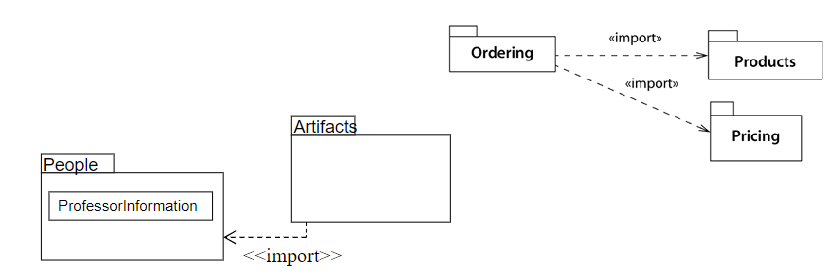
\includegraphics[scale=0.5]{assets/package_import.png}
	\end{center}
	Nota bene:
	\begin{itemize}
		\item La relazione di importazione non è transitiva. Se A importa B e B importa C, allora A può usare (senza qualificarli) gli elementi di B e B può usare (senza qualificarli) gli pubblici di C, ma non è detto che A possa usare (senza qualificarli) gli elementi di C (a meno che A non importi anche C).
		\item Se c'è conflitto di nomi in due elementi importati, nessuno dei due elementi è aggiunto al namespace.
		\item Se il nome di un elemento importato è in conflitto con il nome di un elemento definito localmente (internamente) a un package, il nome dell'elemento interno ha precedenza sul nome importato che non viene aggiunto al namespace (sarà sempre raggiungibile mediante qualificazione).
	\end{itemize}
	I package possono essere innestati senza alcun limite di profondità . Un package innestato ha accesso a tutti gli elementi contenuti direttamente nei package esterni (a qualunque livello di annidamento) senza necessità di importazione. Si può anche specificare la visibilità degli elementi di un package:
	\begin{itemize}
		\item \textbf{public}: visibili ad altri elementi nel package stesso, a uno dei package innestati o a un package che li importano.
		\item \textbf{private}: visibili solo all'interno del package stesso.
	\end{itemize}
	La relazione di importazione può specificare la visibilità di ciò che è importato. Se è pubblica, l'elemento importato è visibilie a qualunque altro elemento che può vedere il package che importa. Se è privata, l'elemento importato non è visibile al di fuori del package che importa.\\
	Per esempio:
	\begin{center}
		\includegraphics[scale=0.5]{assets/package_visibilita.png}
	\end{center}

	\subsection{Classi interne}
	Una classe interna (\textbf{inner class}) è una classe la quale dichiarazione si trova all'interno di un'altra classe ospite (\textbf{top level class}). Le classi interne sono identificate da un nome al pari delle classi top level. \textbf{Una classe interna può essere privata}. In tal caso non è visibile all'esterno della classe ospite. (In java, una classe top level non può mai essere privata). La inner class può \textbf{accedere a tutti i metodi e i campi della classe ospitante}, mentre la classe ospitante può vedere solo la parte pubblica della inner class. \textbf{Un oggetto di classe inner non può esistere se non esiste un oggetto della classe ospitante}. Una classe interna non può avere campi statici. \\
	UML non ha una notazione standard per le classi interne. Si suggerisce la seguente notazione:
	\begin{center}
		\includegraphics[scale=0.5]{assets/classi_interne.png}
	\end{center}

	\subsection{Polimorfismo}
	Il polimorfismo è una caratteristica chiave della programmazione orientata agli oggetti (OOP) che permette di trattare oggetti di classi diverse attraverso un'interfaccia comune. Di seguito approfondiamo i due tipi principali di polimorfismo:
	\begin{itemize}
		\item \textbf{Polimorfismo parametrico}: Questo tipo di polimorfismo si verifica quando una funzione o un metodo può operare con qualsiasi tipo di dato, assumendo che questi tipi condividano una struttura comune. Un esempio classico è una funzione che può operare sia su una lista di interi che su una lista di stringhe. In linguaggi di programmazione come Haskell o Java, questo è ottenuto attraverso l'uso di tipi generici. I tipi generici permettono di scrivere una funzione, una classe o un'interfaccia una sola volta e di utilizzarla con diversi tipi di dati, mantenendo la sicurezza di tipo durante la compilazione.
		\item \textbf{Polimorfismo ad hoc}: Questo tipo di polimorfismo permette di definire funzioni che sembrano lavorare su tipi differenti ma che in realtà sono implementazioni separate per ciascun tipo. Si manifesta principalmente in due forme:
		\begin{itemize}
			\item \textit{Sovraccarico di funzioni}: dove più funzioni con lo stesso nome esistono con parametri differenti. Ad esempio, una funzione \texttt{print()} potrebbe essere definita per stampare sia interi sia stringhe, con un'implementazione specifica per ciascun tipo.
			\item \textit{Specializzazione di funzione}: dove una funzione per un tipo di dati generico viene adattata per gestire tipi di dati più specifici. Questo può comportare un'implementazione totalmente differente che è ottimizzata per un particolare tipo di dati.
		\end{itemize}
	\end{itemize}
	Entrambe le forme di polimorfismo migliorano la flessibilità e la riusabilità del codice. Nel polimorfismo parametrico, la flessibilità è ottenuta tramite l'uso di tipi di dati astratti che possono essere sostituiti con tipi concreti al momento dell'uso. Nel polimorfismo ad hoc, la riusabilità è migliorata permettendo la stessa interfaccia di essere utilizzata per diversi tipi concreti, ciascuno con una propria implementazione specifica.
	Se dovessimo raffinare la classificazione dei diversi meccanismi di polimorfismo adotteremmo la seguente struttura:
	\begin{itemize}
		\item Polimorfismo Universale
		\begin{itemize}
			\item Parametrico
			\item Inclusione
		\end{itemize}
		\item Polimorfismo ad hoc
		\begin{itemize}
			\item Overloading
			\item Coercizione
		\end{itemize}
	\end{itemize}
	Questa classificazione introduce la forma di \textbf{polimorfismo per inclusione} al fine di modellare concetti di sottotipo e di ereditarietà. Il polimorfismo per inclusione e parametrico sono classificati come due sottocategorie del \textbf{polimorfismo Universale} che è posto in contrasto al polimorfismo ad hoc. L'idea del polimorfismo universale è qulla di poter operare su un numero infinito di tipi, a patto che essi rispettino alcuni vincoli. Nel dettaglio, elenchiamo le caratteristiche dei due tipi di polimorfismo:
	\begin{itemize}
		\item Polimorfismo Universale
		\begin{itemize}
			\item è su un numero potenzialmente illimitato di tipi
			\item i diversi morfismi sono generati automaticamente
			\item c'è una base unificante, comune a tutti i diversi morfismi che può assumere l'entità polimorfa
		\end{itemize}
		\item Polimorfismo ad hoc
		\begin{itemize}
			\item è su un numero finito di tipi, spesso pochissimi
			\item i diversi morfismi sono generati in modo manuale o semimanuale
			\item non c'è una base comune a tutti i morfismi, al di la delle intenzioni del progettista (l'uniformità è un caso, non la regola)
		\end{itemize}
	\end{itemize}
	\subsubsection{Coercizione}
	E' il meccanismo di conversione implicita operata da un compilatore per applicare un operatore definito per oggetti di tipo T1 a oggetti di tipo T2. Per esempio in $3.14+5$ l'operatore $+$ è definito per valori reali, ma lo si può usare su un insieme di tipi più grande di quello per il quale è stato definito. Senza coercizione avremmo errore di tipo.\\
	Altri esempi di coercizione sono, in Java per esempio, l'\textbf{autoboxing} di un \textit{int} in un \textit{Integer} e l'\textbf{unboxing} di un \textit{Integer} in un \textit{int}. \\
	Le coercizioni possono essere stabilite staticamente, inserendole automaticamente fra gli argomenti e le funzioni al momento della compilazione, oppure potrebbero essere determinate da test al run-time sugli argomenti. La coercizione è la forma di polimorfismo più semplice. Essa opera a livello semantico cambiando la rappresentazione del dato.
	\subsubsection{Overloading}
	Si ha polimorfismo per \textbf{overloading} quando si usa lo stesso identificatore per metodi differenti e si ricorre a informazioni di contesto per decidere quale metodo è denotato da una particolare occorrenza dell'identificatore. La disambiguaizone necessaria per una corretta compilazione si basa sul tipo degli argomenti del metodo o sulla classe dell'oggetto a cui si richiede il servizio. Possiamo immaginare che una pre-compilazione del programma potrebbe disambiguare ed eliminare l'overloading dando nomi differenti a metodi differenti. L'overloading è giusto una conveniente abbreviazione sintattica. E' presente nella maggior parte dei linguaggi.
	Per esempio:
	\begin{center}
		\includegraphics[scale=0.5]{assets/overloading.png}
	\end{center}
	L'overloading può efficacemente integrare con la coercizione.\\
	Nel paradigma a oggetti si ha overloading anche nel caso di funzioni con medesimo nome ma definite in classi non correlate gerarchicamente.
	\subsubsection{Polimorfismo parametrico}
	Nel poliformismo parametrico, una funzione polimorfa ha un parametro di tipo esplicito o implicito, che determina il tipo dell'argomento per ciascuna applicazione della funzione. Le funzioni che esibiscono il polimorfismo parametrico sono dette anche \textbf{funzioni generiche}. Una funzione generica può lavorare su argomenti di molti tipi, generalmente esibendo lo stesso comportamento indipendentemente dal tipo di argomento. Per esempio:
	\begin{center}
		length(x) = if (x=nil) then 0 else (1+length(tail(x)))
	\end{center}
	La funzione \textbf{length} ha lo stesso comportamento, indipendentemente che si tratti di liste di interi, di reali, di liste ecc.
	\subsubsection{Polimorfismo per inclusione}
	Nasce da una relazione di inclusione fra insiemi di valori. E' tipico dei sottotipi, tuttavia non è necesssariamente legato ai sottotioi. Si ha polimorfismo per inclusione, nella progrmammazione ad oggetti, se un oggetto appartiene a una classe e a tutte le sue superclassi. Esso si manifesta in almeno due modi:
	\begin{itemize}
		\item si può assegnare un oggetto di una qualsiasi sottoclasse di una classe C a una variabile definita di classe C
		\item Una funzione che opera su un oggetto di classe C può essere applicata anche a oggetti di classe C', sottoclasse di C.
	\end{itemize}
	Questi due utilizzi del polimorfismo di inclusione non sono molto distanti dall'utilizzo che permette il concetto di sottotipo anche nella programmazione imperativa. L'utilizzo più interessante si ha quando le invocazioni dei metodi su oggetti di classi diverse, ma gerarchicamente correlate, produce un comportamento differente, anche se la definizione della funzione è unica. Ciò dipende dal \textbf{tipo di legame statico/dinamico} fra identificatore di funzione e relativa realizzazione.
	\vspace{\baselineskip} \\
	Nella maggior parte dei linguaggi di programmazione la visibilità degli identificatori e dei legami (binding) dei nomi alle dichiarazioni è determinata a compile-time. Si parla di \textbf{ambito d'azione statico} (static scope). Nell'ambito d'azione \textbf{dinamico} (dynamic scope), il legame fra l'uso di un identificatore e la sua dichiarazione dipende dall'ordine di esecuzione, e così è differito a run-time.
	\paragraph*{Esempio}
	In Pascal:
	\begin{lstlisting}
		program dynamic(input,output);
		var x: integer;
			procedure A;
			begin
				...;
				write(x);
				...;
			end; {A}
			procedure B;
			var x: real;
			begin
				...;
				A;
				...;
			end; {B}

		begin
			...;
			B;
			...;
			A;
			...;
		end. {dynamic}
	\end{lstlisting}
	Poiché il Pascal adotta la regola dell'ambito statico, l'uso della variabile x in A è legato alla variabile intera x nel programma principale. Questo permette di tradurre la write(X) semplicemente in una chiamata a una funzione di libreria di I/O per la scrittura degli interi. \\
	Tuttavia se il legame nome-dichiarazione fosse dinamico, l'uso di x in A sarebbe vincolato alla dichiarazione di x più recente. Pertanto, quando la procedura A è chiamata dalla procedura B, l'uso di x in A viene vincolato alla dichiarazione della variabile reale x nella procedura B, mentre quando A è chiamata nel programma principale, l'uso di x sarebbe vincolato alla dichiarazione della variabile intera x nel programma principale. \\
	Con un dynamic-binding, la traduzione della chiamata della write(x) può essere determinata solo al run-time. \\
	Questo non vuol dire che il controllo di tipo non possa essere effettuato, ma solo che viene ritardato al momento dell'esecuzione, quando è noto il tipo al quale x è vincolato. \\
	Si osservi che con lo static-binding il legame dei nomi ai tipi (name-type binding) è anch'esso fissato al momento della compilazione.
	\subsubsection{Legame dinamico e polimorfismo di inclusione}
	Nella progrmammazione oo il leame fra nome di funzione e sua realizzazione può essere determinato a run-time. Si consideri il seguente esempio in C++:
	\begin{lstlisting}
		class A{
			public:
				virtual void f() {cout << "A";}
				...
		};
		class B: public A{
			public:
				void f() {cout << "B";} //override
				...
		};
		class Tester{
			public:
				void test(A a) {a.f()...}
		};

		...
		obj1 = new B();
		obj2 = new Tester();
		obj2.test(obj1);
		...
	\end{lstlisting}
	Il comportamento della funzione obj2.test(obj1) dipende da quando si effettua il legame fra l'identificatore di funzione f in test e la sua implementazione. In c++ è possibile definire la funzione f come \textbf{virtuale}, cioè il legame dev essere \textbf{dinamico}, di conseguenza verrà stampata una B. Diversamente, il legame sarebbe \textbf{statico} e verrebbe stampata una A. La selezione del metodo, nel caso di funzioni virtuali, avviene a run-time.
	\paragraph*{Esempio}
	\begin{center}
		\includegraphics[scale=0.5]{assets/binding_dinamico_poli_inclusione.png}
	\end{center}
	Il legame dinamico ci permette di far evolvere il programma aggiungendo nuove sottoclassi di Bird e specificando il codice di move() senza che si modifichi il codice di reLocate() per operare su nuove istanze di nuove sottoclassi di Bird.
	\vspace{\baselineskip} \\
	Combinando polimorfismo di inclusione con legame dinamico si hanno vantaggi di \textbf{estensibilità} di codice.
	\vspace{\baselineskip} \\
	C++ è un esempio di linguaggio dove la tipizzazione è statica ma il legame può essere dinamico (\textbf{statically-typed dynamic binding}). Lo stesso dicasi per Java ma in questo linguaggio \textbf{il legame dinamico è la regola, non l'eccezione}. Solo nei metodi final o static il legame nomedifunzione - realizzazione è statico.
	%%riprendi da slide 125
\end{document}
